\documentclass[12pt,a4paper]{report}

% Essential packages for academic formatting and engineering documentation
\usepackage[utf8]{inputenc}
\usepackage[T1]{fontenc}
\usepackage{geometry}
\geometry{a4paper, margin=1in}
\usepackage{graphicx}
\usepackage{float}
\graphicspath{{images/}}
\usepackage[hyphens]{url}
\usepackage[numbers,sort&compress]{natbib}
\usepackage{xcolor}
\usepackage{listings}
\usepackage{titlesec}
\usepackage{tocbibind} % Automatically adds TOC, LOF, LOT, and bibliography to the Table of Contents

% Redefine chapter titles to appear vertically centered on a dedicated page before content
\titleformat{\chapter}[display]
  {\vspace*{\fill}\normalfont\Huge\bfseries\centering}{\chaptertitlename\ \thechapter}{20pt}{\Huge}[\vspace*{\fill}\clearpage]
\usepackage{longtable}
\usepackage{pifont}
\usepackage{needspace} % Prevent page breaks in listings
\usepackage{rotating} % Landscape tables
\newcommand{\cmark}{\textcolor{green!80!black}{\ding{51}}}%
\newcommand{\xmark}{\textcolor{red}{\ding{55}}}%

% Custom color definitions for clean code listings
\definecolor{codegreen}{rgb}{0,0.6,0}
\definecolor{codegray}{rgb}{0.5,0.5,0.5}
\definecolor{codepurple}{rgb}{0.58,0,0.82}
\definecolor{backcolour}{rgb}{0.95,0.95,0.92}

% Global setup for \begin{lstlisting}
\lstdefinestyle{engineeringstyle}{
    backgroundcolor=\color{backcolour},   
    commentstyle=\color{codegreen},
    keywordstyle=\color{blue},
    numberstyle=\tiny\color{codegray},
    stringstyle=\color{codepurple},
    basicstyle=\ttfamily\footnotesize,
    breakatwhitespace=false,         
    breaklines=true,                 
    captionpos=b,                    
    keepspaces=true,                 
    numbers=left,                    
    numbersep=5pt,                  
    showspaces=false,                
    showstringspaces=false,
    showtabs=false,                  
    tabsize=4
}
\lstset{style=engineeringstyle}

% Define JavaScript and JSON language support
\lstdefinelanguage{JavaScript}{
  keywords={break, case, catch, continue, debugger, default, delete, do, else, finally, for, function, if, in, instanceof, new, return, switch, this, throw, try, typeof, var, void, while, with, let, const, class, export, extends, import, super, async, await},
  morecomment=[l]{//},
  morecomment=[s]{/*}{*/},
  morestring=[b]',
  morestring=[b]",
  sensitive=true
}

\lstdefinelanguage{JSON}{
  keywords={},
  morestring=[b]",
  morecomment=[l]{//},
  morecomment=[s]{/*}{*/}
}

% Define JSX (React syntax)
\lstdefinelanguage{jsx}{
  language=JavaScript,
  morekeywords={const,return,if,async,await}
}

% Define nginx configuration
\lstdefinelanguage{nginx}{
  keywords={server,location,listen,proxy_pass,proxy_set_header,proxy_read_timeout,client_max_body_size,add_header,try_files},
  morecomment=[l]{\#},
  morestring=[b]",
  sensitive=true
}

% Define YAML
\lstdefinelanguage{yaml}{
  keywords={services,image,ports,networks,volumes,environment,depends_on,build,container_name,restart},
  morecomment=[l]{\#},
  morestring=[b]',
  morestring=[b]",
  sensitive=true
}

% Define Dockerfile
\lstdefinelanguage{dockerfile}{
  keywords={FROM,RUN,CMD,EXPOSE,ENV,ADD,COPY,ENTRYPOINT,VOLUME,USER,WORKDIR,ARG,LABEL,HEALTHCHECK,STOPSIGNAL,SHELL},
  morecomment=[l]{\#},
  morestring=[b]",
  sensitive=true
}

% Define Terraform
\lstdefinelanguage{terraform}{
  keywords={resource,variable,output,module,locals,data,provider,terraform,backend,locals},
  morecomment=[l]{\#},
  morestring=[b]",
  sensitive=true
}

% Hyperlink configuration
\usepackage{hyperref}
\hypersetup{
    colorlinks=true,
    linkcolor=blue,
    citecolor=blue,
    filecolor=magenta,      
    urlcolor=cyan,
    pdftitle={Release BSU Engineering Portal - Graduation Project},
    hypertexnames=true,     % Ensure proper link destinations for tables
    bookmarksnumbered=true, % Include chapter/section numbers in bookmarks
}

\begin{document}

% Front Matter (Cover, Abstract, Acknowledgments, TOC)
\pagenumbering{roman}
% Chapter 1: Cover & Formal Pages
% BSU Engineering Portal Graduation Project
% This file contains front matter: Title Page, Abstract, Acknowledgments, TOC setup

% ============================================================================
% 1.1 TITLE PAGE
% ============================================================================

\begin{titlepage}
    % Pull the header to the absolute top of the page
    \vspace*{-1.5cm}
    
    % ================= PROFESSIONAL ACADEMIC HEADER =================
    \noindent
    \begin{minipage}[c]{0.2\textwidth}
        \begin{flushleft}
            
\includegraphics[width=2.5cm]{Beni-Suef_University_logo.png}
        \end{flushleft}
    \end{minipage}
    \hfill
    \begin{minipage}[c]{0.55\textwidth}
        \centering
        {\Large \textbf{Beni-Suef University}}\\[0.15cm]
        {\large Faculty of Engineering}\\[0.15cm]
        {\normalsize Electronics and Communications Engineering Department}
    \end{minipage}
    \hfill
    \begin{minipage}[c]{0.2\textwidth}
        \begin{flushright}
            
\includegraphics[width=2.5cm]{faculty_of_engineering_logo.jpeg}
        \end{flushright}
    \end{minipage}
    
    \vspace{2cm}
    % ================================================================
    
    \centering
    
    % Project Title - Professional Centering
    \vspace{1cm}
    \rule{\textwidth}{1.5pt}\\[0.5cm]
    {\Huge \textbf{Release BSU Engineering Portal}}\\[0.3cm]
    {\Large A Comprehensive Academic Management System}\\[0.5cm]
    \rule{\textwidth}{1.5pt}
    
    \vspace{2.5cm}
    
    % Authors Section
    {\Large \textbf{Prepared by:}}\\[0.3cm]
    {\large Mahmoud Hussein Mahmoud}\\
    {\large Mohamed Gamal Shehata}\\
    {\large Mohamed Essam Sayed}\\[1cm]
    
    {\Large \textbf{Supervised by:}}\\[0.3cm]
    {\large Associate Prof. Dr. Fathy Mostafa}
    
    \vspace{2cm}
    
    % Degree Information
    {\Large \textbf{Graduation Project Report}}\\[0.5cm]
    \noindent {\large Submitted in Partial Fulfillment of the Requirements}\\[0.2cm]
    \noindent {\large for the Degree of Bachelor of Science in}\\[0.2cm]
    \noindent {\large \textbf{Electronics and Communications Engineering}}\\[0.2cm]
    \noindent {\large at Beni-Suef University}\\[1.5cm]
    
    % Academic Year and Date block
    {\Large \textbf{Academic Year 2025--2026}}\\[0.3cm]
    {\large July 2026}
    
\end{titlepage}

% ============================================================================
% 1.2 ABSTRACT
% ============================================================================

\chapter*{Abstract}
\addcontentsline{toc}{chapter}{Abstract}
\label{chap:abstract}

The Faculty of Engineering at Beni-Suef University (BSU) has historically relied on fragmented, Excel-based workflows for academic management---student registration, grade tracking, course assignments, and administrative reporting. This manual approach created severe data inconsistencies across departments, lacked any audit trails for critical administrative actions, and scaled poorly as active enrollment exceeded 4,000 students. The absence of a centralized digital infrastructure not only delayed end-of-semester grade processing but also hindered students' self-service access to essential academic information.

\textbf{Release BSU Engineering Portal} addresses these systemic challenges through a modern, decoupled web architecture comprising: (a) a \textbf{Django 5.0}~\cite{django} backend with Django REST Framework~\cite{djangorest} providing secure, stateless API endpoints with cross-origin Session/CSRF protection; (b) a \textbf{React 19}~\cite{react} frontend built via Vite, utilizing Material-UI~\cite{mui} to deliver highly responsive, state-driven user interfaces; (c) \textbf{MySQL 8.0}~\cite{mysql} as the relational database ensuring strict ACID compliance for grade and attendance transactions; (d) \textbf{Redis}~\cite{redis} for session storage and application-level caching to improve performance and scalability; and (e) \textbf{Docker}~\cite{docker} containerization enabling deterministic, portable deployments across any cloud or on-premises infrastructure.

Key system capabilities include hierarchical academic entity modeling (departments $\rightarrow$ specializations $\rightarrow$ levels $\rightarrow$ students), transaction-safe batch CSV/Excel import pipelines using Pandas for student enrollment and grade uploads, and a highly interactive multi-modal quiz engine. To guarantee data integrity and security, the system enforces the principle of least privilege across eight distinct user roles (Admin, Dean, HOD, Doctor, Student, Student Affairs, Staff Affairs, Graduate Affairs) via custom Role-Based Access Control (RBAC) middleware, coupled with comprehensive audit logging for all administrative actions.

The project demonstrates engineering maturity through robust DevOps practices, security-hardened deployment strategies (configured CORS/CSRF boundaries, input validation, rate limiting), and explicitly defined system boundaries. By abstracting complex administrative workflows into streamlined digital processes, the portal drastically reduces operational overhead, eliminates data silos, and provides a highly scalable foundation for Beni-Suef University's ongoing digital transformation.

\vspace{1cm}
\noindent\textbf{Keywords:} Academic ERP, Django REST Framework, React, Role-Based Access Control (RBAC), Docker, ACID Transactions, Bulk Data Processing, DevOps, Requirements Engineering

% ============================================================================
% 1.3 ACKNOWLEDGMENTS
% ============================================================================

\chapter*{Acknowledgments}
\addcontentsline{toc}{chapter}{Acknowledgments}
\label{chap:acknowledgments}

We extend our deepest gratitude to our supervisor, Associate Prof. Dr. Fathy Mostafa, for his invaluable guidance, patience, and unwavering support throughout this project. His expertise, constructive feedback, and encouragement were instrumental in shaping our technical decisions and ensuring the success of this work.

We also express our appreciation to the faculty members and staff of the Faculty of Engineering, Beni-Suef University, whose insights were vital in understanding the core requirements and operational challenges of the institution.

We acknowledge the robust open-source communities behind Django, React, Pandas, Docker, and the myriad of technologies that form the backbone of this system. Standing on the shoulders of these reliable frameworks allowed us to focus heavily on solving domain-specific institutional challenges without reinventing foundational infrastructure.

Finally, we thank our families and peers for their endless support, continuous encouragement, and patience. Your willingness to beta-test early versions of the portal sustained us through late debugging sessions, complex database migrations, and demanding deadlines.


% ============================================================================
% 1.4 DEDICATION (Optional but recommended)
% ============================================================================

\chapter*{Dedication}
\addcontentsline{toc}{chapter}{Dedication}
\label{chap:dedication}

\textit{To our parents, whose sacrifices made our education possible.}\\[0.5cm]
\textit{To our peers who challenged us to build better systems.}\\[0.5cm]
\textit{And to the students of Beni-Suef University, who deserve efficient, modern tools for their academic journey.}


\tableofcontents
\newpage
\listoffigures
\newpage
\listoftables
\newpage

% Main Content Chapters
\pagenumbering{arabic}
% Chapter 1: Executive Summary / Introduction
% BSU Engineering Portal Graduation Project

\chapter{Executive Summary / Introduction}
\label{chap:introduction}

\section{Problem Statement}
\label{sec:problem-statement}

The Faculty of Engineering at Beni-Suef University (BSU) operates across multiple academic departments---including Electrical Engineering (with EPM and ECE specializations), Mechanical, Civil, and Architecture Engineering---serving thousands of students across five academic levels (Preparatory through Fourth Year). Historically, academic operations relied on fragmented manual workflows characterized by:

\begin{itemize}
    \item \textbf{Excel-based grade management}: Staff Affairs and Student Affairs personnel maintained disjointed spreadsheets for student registration, course assignments, and grade tracking. Version control was non-existent; data inconsistency across departments was the norm.
    \item \textbf{Ad-hoc communication}: Lecture schedules, exam dates, and announcements propagated through informal channels (WhatsApp groups, email chains), leading to information asymmetry between students and faculty.
    \item \textbf{No audit trail}: Administrative actions---batch student uploads, grade modifications, doctor reassignments---left no traceable record, complicating accountability and regression analysis.
    \item \textbf{Paper-heavy processes}: Attendance tracking, quiz administration, and certificate generation required physical document handling, introducing latency and human error.
\end{itemize}

The bottlenecks and disjointed nature of this manual workflow are illustrated in Figure~\ref{fig:current_state}.

\begin{figure}[H]
    \centering
    \includegraphics[width=0.85\textwidth]{images/manual_workflow_1.png}
    \caption{Diagram showing the manual workflow: Staff upload Excel sheets $\rightarrow$ email to department heads $\rightarrow$ manual data entry $\rightarrow$ printed reports.}
    \label{fig:current_state}
\end{figure}

\section{Motivation}
\label{sec:motivation}

The inadequacy of the current solution manifests in three dimensions:

\begin{enumerate}
    \item \textbf{Operational inefficiency}: A single semester's grade finalization required 2--3 weeks of cross-departmental reconciliation. Errors discovered post-publication necessitated manual re-computation of cumulative GPAs for entire cohorts.
    
    \item \textbf{Security and integrity risks}: Uncontrolled Excel file distribution meant sensitive student data (national IDs, grades) resided on personal laptops and unsecured cloud storage. No role-based access control existed---any staff member with a spreadsheet could modify any student's record.
    
    \item \textbf{Scalability ceiling}: As enrollment grew (current $
    \approx$ 4,000 active students), the Excel-based approach approached breaking point. Real-time queries (``What is the current attendance rate for Level 2 Power students?'') required hours of manual aggregation.
\end{enumerate}

The COVID-19 pandemic accelerated the urgency for digital transformation. Remote instruction demanded a centralized platform where:
\begin{itemize}
    \item Doctors could upload lecture materials and administer online quizzes
    \item Students could access schedules, submit quiz attempts, and track grades in real-time
    \item Administrators could execute batch operations (student uploads, grade imports) with full audit logging
\end{itemize}

\section{Proposed Solution}
\label{sec:proposed-solution}

\textbf{Release BSU Engineering Portal} is a web-based academic management system designed as a \textit{single source of truth} for all faculty operations. The system adopts a modern three-tier architecture, as depicted in Figure~\ref{fig:architecture}:

\begin{itemize}
    \item \textbf{Backend}: Django 5.2 with Django REST Framework (DRF), providing a secure, stateless API layer configured for cross-origin integration.
    \item \textbf{Database}: MySQL 8.0 for relational data with ACID compliance
    \item \textbf{Frontend}: React 19 with Material-UI v7, delivered via Vite build tooling
    \item \textbf{Infrastructure}: Docker containerization with Docker Compose orchestration
\end{itemize}

\begin{figure}[H]
    \centering
    \includegraphics[width=0.95\textwidth]{images/system_architecture.png}
    \caption{High-level system architecture showing the React frontend, Nginx reverse proxy, Django REST API, and MySQL database, all encapsulated within a Docker network.}
    \label{fig:architecture}
\end{figure}

\subsection{Key Capabilities}

\begin{enumerate}
    \item \textbf{Role-Based Access Control (RBAC)}: Five distinct roles (Admin, Doctor, Student, Student Affairs, Staff Affairs) with fine-grained permissions enforced via custom DRF permission classes.
    
    \item \textbf{Academic Entity Modeling}: Hierarchical data model supporting departments, specializations (e.g., Electrical $\rightarrow$ EPM/ECE), academic years, terms, and levels with strict referential integrity.
    
    \item \textbf{Fault-Tolerant Batch Operations}: High-performance Excel/CSV import pipelines using Pandas. Operations are wrapped in atomic transactions to guarantee database consistency during partial failures, as demonstrated below:
    \begin{lstlisting}[language=Python, caption=Atomic Transaction for Batch Processing (\texttt{staff\_affairs\_views.py})]
for index, row in df.iterrows():
    try:
        with transaction.atomic():
            national_id = str(row['national_id']).strip()
            # Process individual row safely; rollback on error without halting batch
            if not User.objects.filter(national_id=national_id).exists():
                User.objects.create_user(username=national_id, ...)
    except Exception as e:
        errors.append(f"Row {index + 2}: {str(e)}")
    \end{lstlisting}
    
    \item \textbf{Quiz Engine}: Multi-modal assessment support (MCQ, Essay, Image-based questions) with time limits and automatic grading for objective questions.
    
    \item \textbf{Audit Trail}: Immutable logging of all administrative actions via the \texttt{AuditLog} and \texttt{UploadHistory} models, ensuring complete accountability for grade modifications and user management.
\end{enumerate}

\section{Project Scope}
\label{sec:project-scope}

\subsection{In Scope}

The BSU Engineering Portal will deliver:

\begin{itemize}
    \item Complete student lifecycle management (enrollment $\rightarrow$ course assignment $\rightarrow$ grading $\rightarrow$ certificate generation)
    \item Doctor-facing tools: lecture uploads, schedule management, quiz creation, grade entry
    \item Student-facing portal: schedule viewing, material access, quiz participation, grade inquiry
    \item Administrative dashboards: batch uploads, role management, audit log review, system-wide announcements
    \item Containerized deployment suitable for on-premises or cloud hosting
\end{itemize}

\subsection{Out of Scope (Explicitly Excluded)}

The following items are \textbf{not} addressed in this release:

\begin{itemize}
    \item \textbf{Mobile native applications}: The system provides responsive web access only. iOS/Android apps are deferred to future iterations.
    \item \textbf{Payment processing}: Tuition fees, fines, and financial transactions remain handled by the university's existing ERP system.
    \item \textbf{Real-time chat/video}: Synchronous communication (live lectures, chat) is excluded; integration with external platforms (Zoom, Teams) is preferred.
    \item \textbf{Horizontal auto-scaling}: While containerized, the initial deployment targets single-node operations. The portal focuses on administrative workflows, not pedagogical content delivery.
\end{itemize}

\subsection{Success Metrics}

The project will be evaluated against the following criteria, which are also summarized in Table~\ref{tab:success_metrics}:

\begin{itemize}
    \item \textbf{Functional completeness}: All functional requirements (detailed in Chapter 3) pass User Acceptance Testing (UAT).
    \item \textbf{Performance}: Page load times $<$ 2 seconds for 95th percentile; API response latency $<$ 500ms for authenticated queries
    \item \textbf{Security}: Zero critical vulnerabilities (OWASP Top 10) at production release
    \item \textbf{Adoption}: 100\% of faculty staff and $>$ 80\% of enrolled students actively use the system within one academic semester of deployment
\end{itemize}

\begin{table}[H]
    \centering
    \begin{tabular}{|p{0.3\textwidth}|p{0.2\textwidth}|p{0.25\textwidth}|p{0.15\textwidth}|}
        \hline
        \textbf{Metric} & \textbf{Target} & \textbf{Measurement Method} & \textbf{Responsibility} \\
        \hline
        Functional Completeness & 100\% pass rate & Acceptance Testing & QA Team \\
        API Response Time & $<$ 500ms & Load Testing & Backend \\
        UI Load Time & $<$ 2s (95th \%) & Browser DevTools & Frontend \\
        Security Vulnerabilities & Zero Critical & SAST / DAST Tools & DevOps \\
        \hline
    \end{tabular}
    \caption{Success Metrics Summary}
    \label{tab:success_metrics}
\end{table}

% Chapter 3: Problem Definition & Requirements Engineering
% BSU Engineering Portal Graduation Project

\chapter{Problem Definition \& Requirements Engineering}
\label{chap:requirements}

\section{Current Situation \& Stakeholder Analysis}
\label{sec:current-situation}

\subsection{The Pre-System Workflow}

Prior to the introduction of the BSU Engineering Portal, the Faculty of Engineering at Beni-Suef University operated a predominantly paper-based and spreadsheet-driven academic management process. This workflow exhibited the following systemic failures:

\begin{itemize}
    \item \textbf{Student Records}: Student enrollment data was maintained in Microsoft Excel workbooks, segregated by department and academic year. Adding a single student required manually editing a shared file over the local network, risking data corruption due to concurrent edits.
    \item \textbf{Grade Management}: Faculty members (doctors) recorded attendance and exam grades on paper forms. These forms were physically transported to Student Affairs, where clerks manually re-entered them into another Excel workbook---introducing a high-latency human transcription layer with zero automated validation.
    \item \textbf{Course-Doctor Assignment}: The assignment of faculty members to courses each semester was communicated verbally or via internal paper memos, lacking a central digital record mapping doctors to subjects in the current term.
    \item \textbf{Student Access to Information}: Students lacked a self-service mechanism to view their own grades, attendance records, or exam schedules. They depended entirely on physical notice boards or direct inquiries to Student Affairs, processes that could take days.
    \item \textbf{Audit Trail}: The absence of digital logs meant there was no record of who uploaded grades, who modified student records, or when these actions occurred, making accountability impossible and dispute resolution arbitrary.
\end{itemize}

\subsection{Stakeholder Identification}

Identifying the exact users of the system is the first step in requirements engineering. Table~\ref{tab:stakeholders} identifies every actor in the system, their organizational role, their pain points under the legacy process, and their primary interaction with the proposed portal.

\begin{figure}[H]
    \centering
    \includegraphics[width=\textwidth]{PLACEHOLDER_STAKEHOLDER_DIAGRAM.png}
    \caption{PLACEHOLDER: Insert a Stakeholder Interaction Diagram showing all five roles (Admin, Doctor, Student, Student Affairs, Staff Affairs) and their primary data flows into the centralized system.}
    \label{fig:stakeholders}
\end{figure}

\begin{table}[H]
    \centering
    \renewcommand{\arraystretch}{1.3}
    \begin{tabular}{|p{0.15\textwidth}|p{0.2\textwidth}|p{0.3\textwidth}|p{0.25\textwidth}|}
        \hline
        \textbf{Stakeholder} & \textbf{Organization Role} & \textbf{Pre-System Pain Point} & \textbf{System Interaction} \\
        \hline
        \textbf{Student} & Undergraduate in any dept/level & No self-service access to grades, attendance, or materials. & View grades, attendance, quizzes, schedule, and download lectures. \\
        \hline
        \textbf{Doctor} & Faculty Member teaching courses & No digital tool for recording attendance or publishing quizzes. & Manage courses, record attendance, create quizzes, enter grades. \\
        \hline
        \textbf{Student Affairs} & Admin staff managing student lifecycles & Manual Excel-based registration and redundant grade re-entry. & Batch-upload students, view grades, manage certificates. \\
        \hline
        \textbf{Staff Affairs} & Admin staff managing HR & No structured system for managing doctor course assignments. & Batch-upload doctors, assign to courses, manage deletions. \\
        \hline
        \textbf{Admin} & IT/System Administrator & No central configuration tool; ad-hoc management. & Manage academic years, approve deletions, view audit logs. \\
        \hline
    \end{tabular}
    \caption{Stakeholder Summary and System Interaction Points}
    \label{tab:stakeholders}
\end{table}

\subsection{Stakeholder Permission Boundaries}

A critical engineering decision in the system's design is the enforcement of the \textbf{principle of least privilege}. No single stakeholder role has full system access. Even the Admin role cannot directly enter grades or upload students---those operational capabilities are delegated exclusively to the Doctor and Student Affairs roles, respectively. This ensures that operational authority perfectly matches organizational responsibility.

The following code snippet demonstrates how these boundaries are strictly enforced at the API layer using Django REST Framework permission classes:

\begin{lstlisting}[language=Python, caption=Role-based Permission Guard for Student Affairs (\texttt{permissions.py})]
class IsStudentAffairsRole(permissions.BasePermission):
    """Student Affairs role - exclusively manages students and grades"""
    def has_permission(self, request, view):
        if not request.user or not request.user.is_authenticated:
            return False
        # Admin gets fallback read/write access for administrative support
        return request.user.role in ['STUDENT_AFFAIRS', 'ADMIN']
\end{lstlisting}

\section{Proposed Methodology}
\label{sec:methodology}

\subsection{Why Agile?}

The BSU Engineering Portal was developed using an \textbf{iterative, sprint-based Agile methodology}. A traditional Waterfall approach would have mandated locking all requirements prior to implementation. However, stakeholder interviews frequently revealed new requirements throughout the development cycle. For example, the necessity for a multi-modal quiz engine (supporting MCQ, Essay, and Image-based questions) emerged mid-development when faculty expressed frustration over the lack of integrated online assessment tools.

Agile permitted the engineering team to:
\begin{enumerate}
    \item \textbf{Deliver working features early}: Students could view grades while the quiz engine was still being actively developed.
    \item \textbf{Incorporate feedback incrementally}: The grading template logic was fundamentally redesigned after pilot testing revealed the initial model did not accommodate the faculty's official tertiary grading structure (Coursework / Written / Practical-Oral).
    \item \textbf{Maintain continuous deployment}: Docker containerization ensured every sprint concluded with a highly reproducible, runnable artifact.
\end{enumerate}

\begin{table}[H]
    \centering
    \renewcommand{\arraystretch}{1.2}
    \begin{tabular}{|p{0.15\textwidth}|p{0.3\textwidth}|p{0.45\textwidth}|}
        \hline
        \textbf{Sprint} & \textbf{Focus Area} & \textbf{Key Deliverables} \\
        \hline
        Sprint 1 & Auth \& Core Data & 5-Role User model, login/logout, CSRF, Core Academic Models. \\
        Sprint 2 & Student \& Staff Affairs & Batch Excel uploads (Pandas), student filtering. \\
        Sprint 3 & Course Management & CourseOffering model, doctor assignments, lecture uploads. \\
        Sprint 4 & Attendance \& Grading & Bulk attendance recording, grading templates. \\
        Sprint 5 & Quiz Engine & MCQ/Essay CRUD, auto-grading logic. \\
        Sprint 6 & Student Portal & Dashboards, schedules, grade views. \\
        Sprint 7 & Admin \& Operations & Announcements, audit logging, deletion workflows. \\
        Sprint 8 & DevOps \& Polish & Docker Compose, Nginx proxy, RTL (Arabic) UI support. \\
        \hline
    \end{tabular}
    \caption{Agile Sprint Plan Overview}
    \label{tab:sprints}
\end{table}

\section{Functional Requirements}
\label{sec:functional-reqs}

The following functional requirements are classified using IEEE 830-style prioritization (Must / Should / Could). 

\subsection{Authentication \& User Management}

\begin{itemize}
    \item \textbf{FR-01 [Must]}: The system shall authenticate users via session-based login using a username (national ID) and password.
    \item \textbf{FR-02 [Must]}: The system shall enforce a mandatory password change on first login. The default password shall equal the user's national ID.
    \item \textbf{FR-03 [Must]}: The system shall reject new passwords that match the national ID or are under 6 characters.
    \item \textbf{FR-04 [Must]}: The system shall enforce isolated UI dashboards for all five defined user roles.
    \item \textbf{FR-05 [Must]}: Admin and authorized personnel shall be able to reset any user's password, automatically re-triggering the first-login requirement flag.
\end{itemize}

\begin{lstlisting}[language=Python, caption=Enforcing First-Login Requirement in Model Save (\texttt{models.py})]
def save(self, *args, **kwargs):
    is_new = not self.pk
    if is_new and not self.is_superuser:
        if not self.password or self.password == '!':
            self.set_password(self.national_id or self.username)
        if self.role in ['STUDENT', 'STUDENT_AFFAIRS', 'STAFF_AFFAIRS', 'DOCTOR']:
            self.first_login_required = True
    return super().save(*args, **kwargs)
\end{lstlisting}

\subsection{Student Affairs Operations}

\begin{itemize}
    \item \textbf{FR-06 [Must]}: Upload students in bulk via Excel/CSV (national\_id, full\_name, department, level).
    \item \textbf{FR-07 [Should]}: Provide a pre-flight UI preview of the first 5 rows containing validation errors before committing database writes.
    \item \textbf{FR-08 [Must]}: Validate that Excel data matches dropdown selections (e.g., rejecting a "Mechanical" student uploaded into the "Electrical" form).
    \item \textbf{FR-09 [Must]}: Perform an "upsert" during batch uploads---updating existing records rather than crashing on duplicate national IDs.
    \item \textbf{FR-10 [Must]}: View all student grades globally in a read-only matrix grouped by student and subject.
    \item \textbf{FR-11 [Must]}: Upload zipped PDF graduation certificates, auto-matching filenames (e.g., \texttt{29912...pdf}) to student records.
    \item \textbf{FR-12 [Must]}: Maintain a permanent \texttt{UploadHistory} summarizing created/updated/failed rows per batch.
\end{itemize}

\begin{figure}[H]
    \centering
    \includegraphics[width=\textwidth]{PLACEHOLDER_UPLOAD_PREVIEW.png}
    \caption{PLACEHOLDER: Insert a screenshot of the Student Affairs Upload Form showing the 5-row preview validation step highlighting row errors.}
    \label{fig:upload_preview}
\end{figure}

\subsection{Staff Affairs \& Doctor Operations}

\begin{itemize}
    \item \textbf{FR-13 [Must]}: Staff Affairs shall batch-upload Doctors and assign them to specific \texttt{CourseOfferings} per term.
    \item \textbf{FR-14 [Must]}: Staff Affairs shall submit Doctor deletion requests to the Admin rather than deleting them directly, preventing accidental cascading data loss.
    \item \textbf{FR-15 [Must]}: Doctors shall record bulk attendance for course sessions and export reports.
    \item \textbf{FR-16 [Must]}: Doctors shall enter bulk grades mapped strictly to the course's \texttt{GradingTemplate}.
    \item \textbf{FR-17 [Must]}: Doctors shall create Quizzes (MCQ, Essay, Image). MCQ attempts shall be auto-graded; Essay attempts shall queue for manual doctor review.
\end{itemize}

\section{Non-Functional Requirements}
\label{sec:non-functional-reqs}

Non-functional requirements dictate the system's operational constraints and quality attributes.

\begin{table}[H]
    \centering
    \renewcommand{\arraystretch}{1.3}
    \begin{tabular}{|p{0.1\textwidth}|p{0.15\textwidth}|p{0.45\textwidth}|p{0.2\textwidth}|}
        \hline
        \textbf{ID} & \textbf{Category} & \textbf{Requirement} & \textbf{Target Metric} \\
        \hline
        \textbf{NFR-01} & Security & Passwords hashed via PBKDF2-SHA256. & 0 plaintext DB records \\
        \textbf{NFR-02} & Security & API enforces CSRF protection with \texttt{SameSite=None} cookies for cross-origin integration. & 100\% state mutations verified \\
        \textbf{NFR-03} & Performance & API responses for list endpoints complete in under 2s for datasets $\leq$ 5,000 rows. & $<2$s response time \\
        \textbf{NFR-04} & Usability & Full RTL layout support for Arabic text via MUI plugins. & No broken RTL layouts \\
        \textbf{NFR-05} & Audit & All administrative mutations logged in \texttt{AuditLog}. & 100\% audit coverage \\
        \hline
    \end{tabular}
    \caption{Non-Functional Requirements}
    \label{tab:nfrs}
\end{table}

To protect against brute-force and denial-of-service attempts, rate limiting was configured globally in the backend:

\begin{lstlisting}[language=Python, caption=Global API Rate Limiting Configuration (\texttt{settings.py})]
REST_FRAMEWORK = {
    'DEFAULT_THROTTLE_CLASSES': [
        'rest_framework.throttling.AnonRateThrottle',
        'rest_framework.throttling.UserRateThrottle',
    ],
    'DEFAULT_THROTTLE_RATES': {
        'anon': '100/hour',    # Protects login/public endpoints
        'user': '1000/hour',   # Accommodates heavy batch operations
    },
}
\end{lstlisting}

\section{Use Case Definitions}
\label{sec:use-cases}

\begin{figure}[H]
    \centering
    \includegraphics[width=\textwidth]{PLACEHOLDER_USE_CASE_UML.png}
    \caption{PLACEHOLDER: Insert a UML Use Case Diagram mapping the 5 actors to their respective grouped use cases (Authentication, Academic Mgmt, Quizzes, etc.).}
    \label{fig:use_case_uml}
\end{figure}

\subsection{Detailed Use Case: Batch Student Upload}

This use case outlines the system's most complex data validation pipeline, migrating the faculty away from disjointed Excel hand-offs. A critical engineering decision was made to process rows iteratively inside \texttt{transaction.atomic()} blocks. While Django's \texttt{bulk\_create()} is faster, it fails entirely if a single row errors and obscures row-level validation feedback. The iterative atomic approach allows valid rows to succeed while cleanly capturing exact row indices for failed records.

\textbf{Primary Actor:} Student Affairs\\
\textbf{Main Flow:}
\begin{enumerate}
    \item User selects Department, Academic Year, and Level, then uploads a CSV/Excel file.
    \item System parses the file via Pandas, validating headers and verifying that the file's payload matches the UI dropdown selections (preventing cross-department contamination).
    \item System iterates over rows. If a \texttt{national\_id} exists, the record is updated. If not, a new \texttt{User} and \texttt{Student} record are atomically created.
    \item The system commits an \texttt{UploadHistory} audit log and returns a JSON summary.
\end{enumerate}

\begin{figure}[H]
    \centering
    \includegraphics[width=\textwidth]{PLACEHOLDER_SEQUENCE_UPLOAD.png}
    \caption{PLACEHOLDER: Insert a Sequence Diagram showing the Batch Student Upload flow (Frontend $\rightarrow$ API $\rightarrow$ Pandas Validation $\rightarrow$ Database Transaction $\rightarrow$ AuditLog).}
    \label{fig:seq_upload}
\end{figure}

\subsection{Detailed Use Case: Doctor Deletion Approval Workflow}

Deleting a doctor account cascades destructively through the relational database, removing \texttt{CourseOfferings}, \texttt{StudentGrades}, and \texttt{Attendance} records. To mitigate the risk of catastrophic data loss by administrative error, a \textbf{two-phase approval pattern} was implemented.

\textbf{Main Flow:}
\begin{enumerate}
    \item Staff Affairs initiates a deletion request, providing a required justification.
    \item The API generates a \texttt{DoctorDeletionRequest} marked as \texttt{PENDING}. No data is deleted.
    \item The Admin reviews the request on the Admin Dashboard.
    \item If approved, the Admin triggers the hard deletion and an \texttt{AuditLog} is captured. If rejected, the request is closed and the account remains untouched.
\end{enumerate}

\begin{figure}[H]
    \centering
    \includegraphics[width=0.8\textwidth]{PLACEHOLDER_ADMIN_APPROVAL.png}
    \caption{PLACEHOLDER: Insert a screenshot of the Admin Approval Center showing pending doctor deletion requests with Approve/Reject actions.}
    \label{fig:admin_approval}
\end{figure}

\subsection{Detailed Use Case: Quiz Lifecycle}

The quiz engine represents a fully integrated state machine tracking an assessment from creation to final grading.

\textbf{Main Flow:}
\begin{enumerate}
    \item Doctor provisions a quiz, specifying MCQ or Essay questions and a time limit.
    \item Student starts an attempt; system marks status as \texttt{IN\_PROGRESS}.
    \item Student submits. For MCQ questions, the system instantly calculates scores by comparing choices against the \texttt{is\_correct} boolean flag.
    \item For Essay questions, the attempt is flagged as \texttt{SUBMITTED}. The Doctor must manually review the text payload and assign \texttt{points\_earned}, pushing the status to \texttt{GRADED}.
\end{enumerate}

\begin{lstlisting}[language=Python, caption=Real-time Auto-grading Logic for MCQ Quizzes (\texttt{quiz\_views.py})]
if question.question_type == 'MCQ':
    choice = QuizChoice.objects.get(id=choice_id, question=question)
    answer.selected_choice = choice
    if choice.is_correct:
        answer.points_earned = question.points  # Award full points
        total_score += float(question.points)
    else:
        answer.points_earned = 0                # Incorrect choice
\end{lstlisting}
% Chapter 4: System & Architecture Design
% BSU Engineering Portal Graduation Project

\chapter{System \& Architecture Design}
\label{chap:architecture}

\section{Architecture Overview}
\label{sec:architecture-overview}

\subsection{High-Level Architecture}

The BSU Engineering Portal follows a \textbf{four-tier architecture} pattern, separating concerns into distinct, independently deployable layers to ensure scalability and maintainability:

\begin{enumerate}
    \item \textbf{Presentation Tier}: A React-based Single Page Application (SPA) deployed as a containerized service.
    \item \textbf{API Tier}: A Django REST Framework (DRF) backend, running inside a Gunicorn WSGI server as a scalable AWS ECS Fargate task.
    \item \textbf{Data Tier}: A managed Amazon RDS for MySQL 8.0 instance, providing high availability, automated backups, and automated patching.
    \item \textbf{Routing Tier}: An AWS Application Load Balancer (ALB) acting as the single entry point, routing \texttt{/api/*} requests to the backend service and serving the SPA for all other paths via an Nginx container.
\end{enumerate}

\begin{figure}[H]
    \centering
    \includegraphics[width=0.95\textwidth]{PLACEHOLDER_FOUR_TIER_ARCH.png}
    \caption{PLACEHOLDER: Insert a Cloud Architecture Diagram showing Browser $\leftrightarrow$ AWS ALB $\leftrightarrow$ ECS Fargate Tasks (Nginx/React, Django) $\leftrightarrow$ Amazon RDS (MySQL). Emphasize the AWS VPC and public/private subnet boundaries.}
    \label{fig:four_tier_arch}
\end{figure}

\subsection{Architectural Trade-offs \& Justifications}

\textbf{Why not a Monolith?} \\
A traditional Django monolith renders HTML server-side. While simpler to deploy initially, it fundamentally limits the user experience. The BSU Engineering Portal requires real-time form validation during 500+ row Excel uploads, role-specific dynamic dashboards, and RTL layout support with theme switching. A clean SPA + API split grants full control over the frontend experience while keeping the backend strictly concerned with data and business logic.

\textbf{Why REST over GraphQL?} \\
The system's data access patterns are highly predictable and strictly role-bounded. Each dashboard fetches a well-defined set of resources (e.g., students, grades, courses). GraphQL's flexibility---allowing clients to compose arbitrary queries---is overkill for this domain and introduces unnecessary complexity in resolving granular permission enforcement. With REST, each endpoint is shielded by a single, auditable permission class.

\textbf{Why Amazon RDS \& ECS?} \\
Managing database persistence, backups, and OS patching within standard Docker containers introduces significant operational risk. By offloading data persistence to Amazon RDS, the system guarantees automated point-in-time recovery and Multi-AZ readiness. Utilizing AWS Fargate for the compute tier allows the application containers to run completely serverless, eliminating EC2 host maintenance while maintaining deterministic Docker image deployments.

\begin{table}[H]
    \centering
    \renewcommand{\arraystretch}{1.3}
    \begin{tabular}{|p{0.2\textwidth}|p{0.15\textwidth}|p{0.55\textwidth}|}
        \hline
        \textbf{Layer} & \textbf{Technology} & \textbf{Engineering Justification} \\
        \hline
        \textbf{Frontend} & React 18 & Component-based UI, robust state handling. \\
        \textbf{UI Library} & Material UI v5 & Native RTL capability, Cairo font integration. \\
        \textbf{Backend} & Django 5.x & Mature ORM, session management, reliable auth. \\
        \textbf{API Framework} & DRF 3.x & Seamless serialization, extensible permission classes. \\
        \textbf{Database} & MySQL 8.0 & ACID compliance for strict academic records. \\
        \textbf{Infrastructure} & AWS ECS (Fargate) \& RDS & Serverless container compute, zero-maintenance managed database. \\
        \hline
    \end{tabular}
    \caption{Technology Stack \& Engineering Justification}
    \label{tab:tech_stack}
\end{table}

\subsection{Cloud Deployment Topology (AWS)}

The production deployment abandons single-host limitations in favor of a cloud-native approach using Amazon Web Services (AWS). Compute resources are orchestrated via \textbf{Elastic Container Service (ECS) with AWS Fargate}.

A critical security decision was the \textbf{Virtual Private Cloud (VPC) isolation strategy}. The architecture employs logically isolated networks:
\begin{itemize}
    \item \textbf{Public Subnet}: Hosts the Application Load Balancer (ALB), which intercepts external HTTPS traffic and acts as a shield against DDoS attacks.
    \item \textbf{Private Subnet (Compute)}: Hosts the ECS Fargate tasks (Frontend and Backend). These tasks are not assigned public IP addresses and can only be reached via the ALB.
    \item \textbf{Private Subnet (Data)}: Hosts the Amazon RDS MySQL instance. Its Security Group strictly permits ingress traffic exclusively on port 3306 originating from the backend Fargate task's Security Group, neutralizing direct external database attacks.
\end{itemize}

\begin{lstlisting}[language=json, caption=ECS Task Definition Snippet injecting secrets via AWS Systems Manager (\texttt{task-def.json})]
"containerDefinitions": [
  {
    "name": "bsu-backend",
    "image": "123456789.dkr.ecr.eu-west-1.amazonaws.com/bsu-backend:latest",
    "portMappings": [{"containerPort": 8000, "protocol": "tcp"}],
    "secrets": [
      { "name": "DB_PASSWORD", "valueFrom": "arn:aws:ssm:region:account:parameter/db_pass" }
    ]
  }
]
\end{lstlisting}

\section{System Modeling (UML)}
\label{sec:system-modeling}

\subsection{Sequence Diagram: Authentication \& CSRF Handshake}

Because the SPA and API are decoupled, session-based authentication requires a deliberate Cross-Site Request Forgery (CSRF) handshake. The browser must retrieve a CSRF token cookie before dispatching the POST request containing credentials.

\begin{figure}[H]
    \centering
    \includegraphics[width=\textwidth]{PLACEHOLDER_AUTH_SEQUENCE.png}
    \caption{PLACEHOLDER: Insert a Sequence Diagram for Login \& CSRF Handshake (Browser $\rightarrow$ Nginx $\rightarrow$ Django: GET /api/auth/csrf/ $\rightarrow$ POST /api/auth/login/).}
    \label{fig:seq_auth}
\end{figure}

\subsection{Activity Diagram: Fault-Tolerant Batch Operations}

Batch uploads (e.g., student enrollment, attendance logs) are the system's most data-intensive operations. Rather than rejecting an entire 500-row file due to a single invalid row, the system utilizes iterative row-level processing. As demonstrated in the \texttt{BulkAttendanceView}, the system traps operational exceptions per row without halting the broader batch execution.

\begin{figure}[H]
    \centering
    \includegraphics[width=\textwidth]{PLACEHOLDER_BATCH_ACTIVITY.png}
    \caption{PLACEHOLDER: Insert an Activity Diagram for Batch Uploads showing file selection, Pandas parsing, row iteration, isolated database commits, and error aggregation.}
    \label{fig:act_batch}
\end{figure}

\begin{lstlisting}[language=Python, caption=Row-level Fault Tolerance during Batch Insert (\texttt{academic/views.py})]
for idx, item in enumerate(attendance_list):
    try:
        # Process row safely; isolate errors without halting batch
        obj, is_created = Attendance.objects.update_or_create(
            student=student, course_offering=course_offering,
            date=date, defaults={'status': attendance_status}
        )
    except Exception as e:
        errors.append(f"Row {idx+1}: {str(e)}")
\end{lstlisting}

\subsection{State Machine: Quiz Lifecycle}

The assessment subsystem treats quizzes as a state machine. A student attempt transitions through four distinct states. Objectively graded quizzes (MCQs) transition directly to \texttt{GRADED}, whereas essay responses remain \texttt{SUBMITTED} pending manual doctor review.

\begin{lstlisting}[language=Python, caption=Quiz Attempt State Machine in Django Model (\texttt{academic/models.py})]
class StudentQuizAttempt(models.Model):
    class AttemptStatus(models.TextChoices):
        IN_PROGRESS = 'IN_PROGRESS', 'جاري الحل'
        SUBMITTED   = 'SUBMITTED', 'تم التسليم'
        TIMEOUT     = 'TIMEOUT', 'انتهى الوقت'
        GRADED      = 'GRADED', 'تم التصحيح'

    status = models.CharField(max_length=20, choices=AttemptStatus.choices)
\end{lstlisting}

\begin{figure}[H]
    \centering
    \includegraphics[width=0.8\textwidth]{PLACEHOLDER_QUIZ_STATE_MACHINE.png}
    \caption{PLACEHOLDER: Insert a State Machine Diagram for Quiz Lifecycle (IN\_PROGRESS $\rightarrow$ SUBMITTED $\rightarrow$ GRADED, with TIMEOUT branch).}
    \label{fig:quiz_state}
\end{figure}

\section{Database Design}
\label{sec:database-design}

\subsection{Entity-Relationship Overview}

The database is heavily normalized into over 20 tables, organized into five functional domains to ensure a clean separation of concerns:

\begin{enumerate}
    \item \textbf{Identity \& Access}: Manages user accounts and role-based permissions.
    \item \textbf{Academic Structure}: Defines the faculty's static hierarchy (Departments, Subjects, etc.).
    \item \textbf{Academic Operations}: Contains transactional data like grades and attendance.
    \item \textbf{Assessment}: The complete quiz engine schema.
    \item \textbf{System \& Communication}: Handles system-level features like audit logs and announcements.
\end{enumerate}

\begin{figure}[H]
    \centering
    \includegraphics[width=\textwidth]{PLACEHOLDER_ERD_FULL.png}
    \caption{PLACEHOLDER: Insert the full Entity-Relationship Diagram (ERD) detailing primary keys, foreign keys, and cardinalities across the schema.}
    \label{fig:erd_full}
\end{figure}

\subsection{The CourseOffering Pivot Entity}

The \texttt{CourseOffering} model represents the architectural cornerstone of the academic domain. It serves as a central junction tying together a \texttt{Subject}, a \texttt{Doctor}, an \texttt{AcademicYear}, a \texttt{Term}, and a \texttt{Level}. All subsequent operational data (Lectures, Quizzes, Attendance, Grades) hang off this central pivot rather than directly off a subject.

\begin{lstlisting}[language=Python, caption=CourseOffering Pivot Entity Definition (\texttt{academic/models.py})]
class CourseOffering(models.Model):
    subject = models.ForeignKey(Subject, on_delete=models.CASCADE)
    academic_year = models.ForeignKey(AcademicYear, on_delete=models.CASCADE)
    level = models.ForeignKey(Level, on_delete=models.CASCADE)
    doctor = models.ForeignKey(User, limit_choices_to={'role': 'DOCTOR'})
    
    class Meta:
        unique_together = ('subject', 'academic_year', 'term', 'level')
\end{lstlisting}

This composite \texttt{unique\_together} constraint enforces a critical business rule at the database level: a specific subject cannot be duplicated for the same level within the same academic term.

\subsection{Dual Identity: User vs. Student}

A deliberate separation of concerns was implemented by decoupling the authentication model (\texttt{User}) from the academic metadata model (\texttt{Student}) using a \texttt{OneToOneField}. This design was chosen over embedding academic fields directly into the User model for two key reasons:

\begin{enumerate}
    \item \textbf{Separation of Concerns}: Authentication data (password hash, role, session tokens) belongs to the \texttt{User} model. Academic data (level, department, grades) belongs to the \texttt{Student} model. This prevents the core authentication entity from being polluted with domain-specific properties.
    \item \textbf{Lifecycle Independence}: A Student record can be managed or even deleted (e.g., upon graduation) without destroying the underlying User account, preserving a historical record if needed.
\end{enumerate}

\begin{lstlisting}[language=Python, caption=Decoupled Student and User Models (\texttt{academic/models.py})]
class Student(models.Model):
    user = models.OneToOneField(User, on_delete=models.CASCADE,
                                related_name='student_profile')
    level = models.ForeignKey(Level, on_delete=models.SET_NULL, ...)
    department = models.ForeignKey(Department, on_delete=models.SET_NULL, ...)
\end{lstlisting}

\subsection{Assessment Schema Design}

The quiz subsystem follows a nested composition pattern, where a \texttt{Quiz} contains multiple \texttt{QuizQuestion}s, which in turn can have multiple \texttt{QuizChoice}s. Student interactions are tracked via the \texttt{StudentQuizAttempt} and \texttt{StudentQuizAnswer} models, forming a relational structure that is both queryable and auditable.

\begin{table}[H]
    \centering
    \renewcommand{\arraystretch}{1.3}
    \begin{tabular}{|l|l|l|}
        \hline
        \textbf{Table} & \textbf{Key Columns} & \textbf{Purpose} \\ \hline
        \texttt{Quiz} & \texttt{course\_offering\_id, quiz\_type, total\_points} & Defines the assessment container. \\
        \texttt{QuizQuestion} & \texttt{quiz\_id, question\_type, points} & Stores an individual question (MCQ/ESSAY). \\
        \texttt{QuizChoice} & \texttt{question\_id, is\_correct} & Stores a possible answer for an MCQ question. \\
        \texttt{StudentQuizAttempt} & \texttt{student\_id, quiz\_id, score, status} & Tracks a single student's attempt at a quiz. \\
        \texttt{StudentQuizAnswer} & \texttt{attempt\_id, question\_id, selected\_choice\_id} & Records a student's answer to one question. \\ \hline
    \end{tabular}
    \caption{Summary of the Quiz Subsystem Schema}
    \label{tab:quiz_schema}
\end{table}

\subsection{Normalization and Database Integrity}

The schema is normalized to Third Normal Form (3NF) to eliminate data redundancy and prevent update anomalies. Business rules are enforced at the database level using composite unique constraints, which are more reliable than application-level checks, especially under concurrent write operations.

\begin{table}[H]
    \centering
    \renewcommand{\arraystretch}{1.3}
    \begin{tabular}{|p{0.25\textwidth}|p{0.35\textwidth}|p{0.3\textwidth}|}
        \hline
        \textbf{Table} & \textbf{Composite Unique Constraint} & \textbf{Business Rule Validated} \\
        \hline
        \texttt{Attendance} & \texttt{(student, course\_offering, date)} & One attendance record per session. \\
        \hline
        \texttt{StudentGrade} & \texttt{(student, course\_offering)} & One master grade sheet per course. \\
        \hline
        \texttt{StudentQuizAttempt} & \texttt{(student, quiz)} & Strict single-attempt policy. \\
        \hline
        \texttt{StudentQuizAnswer} & \texttt{(attempt, question)} & One answer per question per attempt. \\
        \hline
        \texttt{Term} & \texttt{(name, academic\_year)} & Prevents duplicate terms (e.g., two "First" terms) in one year. \\
        \hline
    \end{tabular}
    \caption{Key Composite Constraints Enforcing Database Integrity}
    \label{tab:db_constraints}
\end{table}

\section{Backend Design}
\label{sec:backend-design}

\subsection{Application Structure \& Namespace}

The backend follows a modular monolith structure, organized into four distinct Django applications, each with a single responsibility. This modularity prevents the codebase from becoming a tangled "big ball of mud" and clarifies ownership.

\begin{verbatim}
backend/
├── bsu_backend/  # Project settings, WSGI, root URL config
├── users/        # Authentication, user models, RBAC permissions
├── academic/     # Core academic operations (largest module)
├── content/      # CMS-like features (News, Announcements)
└── system/       # System-level operations (Audit Logs)
\end{verbatim}

Routing is encapsulated under dedicated API namespaces to ensure predictable and maintainable URL structures. For instance, all 120+ endpoints handling faculty workflows live under the \texttt{/api/academic/} boundary, while authentication endpoints are grouped under \texttt{/api/auth/}.

\begin{figure}[H]
    \centering
    \includegraphics[width=0.75\textwidth]{PLACEHOLDER_BACKEND_MODULES.png}
    \caption{PLACEHOLDER: Insert a Dependency Diagram showing the modular structure of the Django apps (users $\rightarrow$ academic $\rightarrow$ system).}
    \label{fig:backend_modules}
\end{figure}

\subsection{Middleware Pipeline}

HTTP requests transit through an explicit middleware sequence defined in \texttt{settings.py}. The configuration order is structurally critical for security and functionality. For example, \texttt{CorsMiddleware} must execute before most other middleware to ensure that CORS preflight (OPTIONS) requests are handled correctly without being blocked by security checks.

\begin{lstlisting}[language=Python, caption=Critical Middleware Order in \texttt{settings.py}]
MIDDLEWARE = [
    'corsheaders.middleware.CorsMiddleware',        # 1. Must be high for preflight checks
    'django.middleware.security.SecurityMiddleware',
    'whitenoise.middleware.WhiteNoiseMiddleware',
    'django.contrib.sessions.middleware.SessionMiddleware',
    'django.middleware.common.CommonMiddleware',
    'django.middleware.csrf.CsrfViewMiddleware',
    'django.contrib.auth.middleware.AuthenticationMiddleware',
    'django.contrib.messages.middleware.MessageMiddleware',
    'django.middleware.clickjacking.XFrameOptionsMiddleware',
]
\end{lstlisting}

\subsection{Defense in Depth: Three-Tier Authorization}

Security is not delegated to a single layer. Instead, Role-Based Access Control (RBAC) relies on three sequential verifications:

\begin{enumerate}
    \item \textbf{Routing Gateway}: Nginx segregates API requests from static asset requests.
    \item \textbf{View-Level Permissions}: DRF viewsets dynamically assign permission classes based on the requested HTTP verb (\texttt{action}). Read operations may be allowed for authenticated users, while mutations are restricted to specific staff roles.
\end{enumerate}

\begin{lstlisting}[language=Python, caption=Dynamic Class-Level Permission Resolution (\texttt{academic/views.py})]
class CourseOfferingViewSet(viewsets.ModelViewSet):
    def get_permissions(self):
        if self.action in ['create', 'update', 'partial_update', 'destroy']:
            return [IsStaffAffairsRole()]
        return [permissions.IsAuthenticated()]
\end{lstlisting}

\begin{enumerate}
    \setcounter{enumi}{2}
    \item \textbf{Object-Level Ownership}: Even if a user has the \texttt{DOCTOR} role, the system queries the relational hierarchy to verify ownership of the specific resource being mutated.
\end{enumerate}

\begin{lstlisting}[language=Python, caption=Object-Level Ownership Verification (\texttt{academic/views.py})]
course_offering = CourseOffering.objects.get(id=course_offering_id)
# Prevent cross-doctor grade tampering
if not request.user.is_superuser and course_offering.doctor != request.user:
    return Response({'error': 'Not authorized'}, status=status.HTTP_403_FORBIDDEN)
\end{lstlisting}

\subsection{Immutable Audit Logging}

Administrative confidence requires traceability. All critical mutations processed by administrative roles generate an \texttt{AuditLog} record. This model leverages Django's \texttt{JSONField} to store context-aware payloads mapping specifically to the event signature. This provides far more useful information than a simple text message.

\begin{lstlisting}[language=Python, caption=AuditLog Model with Flexible JSONField (\texttt{system/models.py})]
class AuditLog(models.Model):
    class ActionType(models.TextChoices):
        STUDENT_BATCH_UPLOAD = "STUDENT_BATCH_UPLOAD"
        DOCTOR_ASSIGNMENT    = "DOCTOR_ASSIGNMENT"
        GRADE_APPROVED       = "GRADE_APPROVED"
        # ... other action types

    action = models.CharField(max_length=50, choices=ActionType.choices)
    performed_by = models.ForeignKey(User, ...)
    details = models.JSONField(null=True, blank=True) # Context-specific data
\end{lstlisting}

For example, a \texttt{STUDENT\_BATCH\_UPLOAD} action stores a payload of \texttt{\{"created": 50, "updated": 5, "errors": 2\}}, while a \texttt{DOCTOR\_ASSIGNMENT} action stores \texttt{\{"doctor\_name": "...", "subject": "..."\}}.

\section{Frontend \& UI/UX Design}
\label{sec:frontend-design}

\subsection{State Management \& Architecture}

The application eschews heavy state libraries like Redux in favor of the native \textbf{React Context API}. State is session-scoped (authentication context, UI theme context) rather than deeply interconnected. The primary \texttt{AuthProvider} performs a background session validation immediately on load to prevent UI hydration flashes.
\begin{lstlisting}[language=JavaScript, caption=Session Revalidation in AuthProvider]
useEffect(() => {
    const storedUser = localStorage.getItem('user');
    if (storedUser) {
        api.get('/api/auth/profile/')
            .then(res => setUser(res.data)) // Session is valid
            .catch(() => {
                localStorage.removeItem('user'); // Session expired
                setUser(null);
            });
    }
}, []);
\end{lstlisting}
\begin{figure}[H]
    \centering
    \includegraphics[width=0.85\textwidth]{PLACEHOLDER_REACT_TREE.png}
    \caption{PLACEHOLDER: Insert a React Component Tree Diagram demonstrating the Context Provider nesting (Theme $\rightarrow$ Auth $\rightarrow$ Router) shielding the functional components.}
    \label{fig:react_tree}
\end{figure}

\subsection{Route Protection}

A custom \texttt{<ProtectedRoute>} wrapper component enforces client-side authorization barriers. It sequentially validates three conditions before rendering a protected page:
\begin{enumerate}
    \item \textbf{Authentication}: Is a user object present in the \texttt{AuthContext}?
    \item \textbf{First Login}: Is the user's \texttt{first\_login\_required} flag set to true?
    \item \textbf{Role Authorization}: Does the user's role exist in the route's allowed roles array?
\end{enumerate}
If any check fails, the user is redirected to the appropriate page (\texttt{/login}, \texttt{/change-password}, or the home page).

\begin{lstlisting}[language=jsx, caption=ProtectedRoute Component Logic]
const ProtectedRoute = ({ children, roles }) => {
    const { user } = useAuth();
    if (!user) return <Navigate to="/login" replace />;
    if (user.first_login_required) return <Navigate to="/change-password" replace />;
    if (roles && !roles.includes(user.role)) return <Navigate to="/" replace />;
    return children;
};
\end{lstlisting}

\begin{lstlisting}[language=JavaScript, caption=API Request Interception for Expiry Handling]
api.interceptors.response.use(
    (response) => response,
    (error) => {
        if (error.response?.status === 401) {
            localStorage.removeItem('user');
            window.location.href = '/login'; // Force re-authentication
        }
        return Promise.reject(error);
    }
);
\end{lstlisting}

\subsection{RTL-First Interface \& Theming}

Because the faculty requires an Arabic-native interface, the UI was built RTL-first. It leverages Material-UI's built-in RTL support, which uses the \texttt{stylis-plugin-rtl} library to automatically mirror CSS properties (e.g., converting \texttt{padding-left} to \texttt{padding-right}) when the theme's direction is set to \texttt{'rtl'}. The design incorporates the "Cairo" Google Font, which is heavily optimized for Arabic script legibility. Dark mode integration maps the university's primary color palette to low-luminance backgrounds to reduce eye strain.

\begin{figure}[H]
    \centering
    \includegraphics[width=\textwidth]{PLACEHOLDER_THEME_COMPARISON.png}
    \caption{PLACEHOLDER: Insert a side-by-side screenshot comparing the complex Student Dashboard in Light Mode vs. Dark Mode.}
    \label{fig:theme_compare}
\end{figure}

\subsection{Build Optimization \& Deployment}

The project utilizes multi-stage Docker builds to create lean, production-optimized container images. The frontend build process, for example, uses a Node.js image to build the static React assets, then copies only the resulting \texttt{/dist} folder and the Nginx configuration into a lightweight \texttt{nginx:alpine} image for the final artifact. This ensures the production container has a minimal attack surface and does not contain any build-time dependencies.

The backend container's \texttt{entrypoint.sh} script automates critical startup tasks, including running database migrations and collecting static files, before starting the Gunicorn server.

\subsection{Reverse Proxy Engineering}

The Nginx container serves a dual purpose: it efficiently serves the static frontend assets and acts as a reverse proxy for the backend API. This single-entrypoint architecture simplifies CORS configuration and network security. The Nginx configuration is engineered to handle large file uploads and support client-side routing.

\begin{lstlisting}[language=nginx, caption=Nginx Reverse Proxy Configuration (\texttt{nginx.conf})]
server {
    listen 80;
    client_max_body_size 50M; # Allow large file uploads

    # Route for React SPA (client-side routing)
    location / {
        try_files $uri $uri/ /index.html;
    }

    # Route for Django API
location /api/ {
        proxy_pass http://backend:8000; # Forward to backend service
        proxy_set_header X-Real-IP $remote_addr;
        proxy_read_timeout 300s; # Accommodate long-running batch uploads
    }
}
\end{lstlisting}
% Chapter 5: Security Design
% BSU Engineering Portal Graduation Project

\chapter{Security Design}
\label{chap:security}

Security in the BSU Engineering Portal is not treated as a bolt-on feature, but rather as a structural property woven into every layer of the architecture. From session management at the protocol level to database isolation at the infrastructure level, each design decision was governed by the principle of \textbf{defense in depth}---ensuring that every layer is independently defensible.

\section{Authentication and Session Management}
\label{sec:auth-session}

\subsection{Why Session-Based Authentication Over JWT}

The most consequential security decision in the system's design was the selection of \textbf{Session-Based Authentication} over JSON Web Tokens (JWT)~\cite{jwt}. While JWT is popular in modern SPA architectures, it was deliberately rejected after an architectural trade-off analysis specific to the faculty's operational requirements.

\begin{table}[H]
    \centering
    \renewcommand{\arraystretch}{1.3}
    \begin{tabular}{|p{0.25\textwidth}|p{0.35\textwidth}|p{0.35\textwidth}|}
        \hline
        \textbf{Criterion} & \textbf{Session-Based (Chosen)} & \textbf{JWT (Rejected)} \\
        \hline
        \textbf{Server-side invalidation} & Immediate. Destroying the session instantly logs the user out. & Impossible without a Redis blacklist; compromised tokens remain valid until expiry. \\
        \hline
        \textbf{Forced password change} & Natural flow. Session is destroyed, forcing immediate re-login. & Requires complex token revocation infrastructure. \\
        \hline
        \textbf{Admin password reset} & Simple. Reset password + wipe active session keys. & Old JWT remains valid until expiry, allowing continued unauthorized access. \\
        \hline
        \textbf{Token lifecycle} & Managed natively by Django middleware. & Requires access/refresh rotation logic and secure storage handling. \\
        \hline
    \end{tabular}
    \caption{Authentication Architecture Trade-off Analysis}
    \label{tab:auth_tradeoff}
\end{table}

The decisive factor was the institution's strict password lifecycle. Administrators frequently reset student passwords to their National ID, forcing a password change on the next login. Sessions allow this to happen instantly and atomically, whereas JWT would require significant additional infrastructure to achieve the same immediate revocation.

\subsection{Cross-Origin Session Configuration}

Because the application utilizes a decoupled SPA architecture (e.g., React on a separate origin or port from Django), the session cookies must traverse origins securely.

\begin{lstlisting}[language=Python, caption=Session Cookie Configuration (\texttt{settings.py})]
# Required for cross-origin cookie sending in SPA architectures
SESSION_COOKIE_SAMESITE = 'None'   
# Required when SameSite=None; ensures cookies are only sent over HTTPS
SESSION_COOKIE_SECURE = True       
\end{lstlisting}

\subsection{Login and Logout Flows}

The login endpoint creates a server-side session and returns the user profile, crucially including a \texttt{first\_login\_required} flag which the frontend uses for immediate routing. Conversely, the logout flow emphasizes security by executing a dual-cleanup process.

\begin{lstlisting}[language=JavaScript, caption=Dual-Cleanup Logout Flow (\texttt{AuthContext.jsx})]
const logout = async () => {
    try {
        await api.post('/api/auth/logout/'); // 1. Destroy server-side session
    } catch {
        // Continue client-side logout even if backend is unreachable
    }
    localStorage.removeItem('user');         // 2. Clear client UI state
    setUser(null);
};
\end{lstlisting}

\subsection{Session Storage Security (Redis)}

Sessions are stored in a container-local Redis 7.x instance rather than file-based storage. This design provides both performance benefits (sub-millisecond session reads) and security advantages over traditional file-based session backends.

\begin{lstlisting}[language=Python, caption=Redis Session Backend Configuration (\texttt{settings.py})]
# Redis as session backend (in-memory, no persistence requirement)
SESSION_ENGINE = "django.contrib.sessions.backends.cache"
SESSION_CACHE_ALIAS = "default"

# Cache configuration pointing to local Redis
CACHES = {
    "default": {
        "BACKEND": "django_redis.cache.RedisCache",
        "LOCATION": os.environ.get('REDIS_URL', 'redis://redis:6379/1'),
        "OPTIONS": {
            "CLIENT_CLASS": "django_redis.client.DefaultClient",
        }
    }
}
\end{lstlisting}

Key security properties of this design:
\begin{itemize}
    \item \textbf{Network Isolation:} Redis binds only to localhost (127.0.0.1:6379), rejecting all external connections
    \item \textbf{No Persistence:} Sessions exist only in memory; container restart clears all session data (forced re-authentication)
    \item \textbf{Automatic Expiry:} Redis TTL matches Django \texttt{SESSION\_COOKIE\_AGE} (default 2 weeks), automatically pruning stale sessions
    \item \textbf{Sidecar Pattern:} Redis runs in the same ECS task, eliminating network traversal risks
\end{itemize}

\section{Role-Based Authorization (RBAC)}
\label{sec:rbac}

\subsection{The Role Model and Permission Classes}

The system implements an \textbf{eight-role authorization model} (Admin, Dean, HOD, Doctor, Student, Student Affairs, Staff Affairs, Graduate Affairs). Authorization is enforced at the backend through ten custom Django REST Framework (DRF) [2] permission classes. 

A key design decision was to grant the Admin role inherited capabilities across all administrative views. Rather than relying on a complex hierarchical tree, this inheritance is made explicit in each permission class for strict auditability.

\begin{lstlisting}[language=Python, caption=Explicit Role Inheritance (\texttt{permissions.py})]
class IsStudentAffairsRole(permissions.BasePermission):
    """Student Affairs role - manages students and grades"""
    def has_permission(self, request, view):
        if not request.user or not request.user.is_authenticated:
            return False
        # Admin inherits access explicitly
        return request.user.role in ['STUDENT_AFFAIRS', 'ADMIN']
\end{lstlisting}

\subsection{Frontend Route Protection vs. Backend Enforcement}

Authorization operates at two distinct layers. The frontend utilizes a \texttt{\textless ProtectedRoute\textgreater} wrapper to route users away from unauthorized views and handle the mandatory password change redirect.

However, the architectural principle holds that \textbf{frontend route protection is merely a UX convenience}. A determined attacker can bypass client-side JavaScript. True security relies on the backend endpoints evaluating the session's role payload against the requested resource.

\begin{sidewaystable}
    \centering
    \renewcommand{\arraystretch}{1.2}
    \caption{Role-Based Access Control (RBAC) Permission Matrix}
    \label{tab:rbac_matrix}
    \begin{tabular}{|p{0.22\textwidth}|c|c|c|c|c|c|c|c|}
        \hline
        \textbf{Operation} & \textbf{Admin} & \textbf{Dean} & \textbf{HOD} & \textbf{Doctor} & \textbf{Student} & \textbf{Student Aff.} & \textbf{Staff Aff.} & \textbf{Grad Aff.} \\
        \hline
        User Management & \cmark & \xmark & \xmark & \xmark & \xmark & \xmark & \xmark & \xmark \\ \hline
        Academic Year CRUD & \cmark & \xmark & \xmark & \xmark & \xmark & \xmark & \xmark & \xmark \\ \hline
        Department CRUD & \cmark & \xmark & \xmark & \xmark & \xmark & \xmark & \xmark & \xmark \\ \hline
        Upload Students & \cmark & \xmark & \xmark & \xmark & \xmark & \cmark & \xmark & \xmark \\ \hline
        Upload Doctors & \cmark & \xmark & \xmark & \xmark & \xmark & \xmark & \cmark & \xmark \\ \hline
        Assign Doctor & \cmark & \xmark & \cmark & \xmark & \xmark & \xmark & \xmark & \xmark \\ \hline
        Enter Grades & \cmark & \xmark & \xmark & \cmark (Own) & \xmark & \xmark & \xmark & \xmark \\ \hline
        Upload Exam Grades & \cmark & \xmark & \xmark & \xmark & \xmark & \cmark & \xmark & \xmark \\ \hline
        Publish Results & \cmark & \cmark & \xmark & \xmark & \xmark & \xmark & \xmark & \xmark \\ \hline
        Take Quizzes & \xmark & \xmark & \xmark & \xmark & \cmark & \xmark & \xmark & \xmark \\ \hline
        View Own Grades & \xmark & \xmark & \xmark & \xmark & \cmark & \xmark & \xmark & \xmark \\ \hline
        Manage News & \cmark & \xmark & \xmark & \xmark & \xmark & \cmark & \cmark & \xmark \\ \hline
        Manage Certificates & \cmark & \xmark & \xmark & \xmark & \xmark & \xmark & \xmark & \cmark \\ \hline
        Manage Clearance & \cmark & \xmark & \xmark & \xmark & \xmark & \xmark & \xmark & \cmark \\ \hline
        Manage Career Portal & \cmark & \xmark & \xmark & \xmark & \xmark & \xmark & \xmark & \cmark \\
        \hline
    \end{tabular}
\end{sidewaystable}

\section{Password Security}
\label{sec:password-security}

\subsection{Hashing and Validation}

Passwords are never stored in plaintext. The system leverages Django's [1] \texttt{PBKDF2-SHA256} hashing algorithm with a 720,000-iteration key derivation function [25]. Furthermore, four strict validators intercept all password creations:

\begin{itemize}
    \item \texttt{UserAttributeSimilarityValidator}: Rejects passwords matching the National ID.
    \item \texttt{MinimumLengthValidator}: Enforces a baseline 8-character length.
    \item \texttt{CommonPasswordValidator}: Rejects over 20,000 universally breached passwords.
    \item \texttt{NumericPasswordValidator}: Prohibits strictly numerical inputs.
\end{itemize}

\subsection{The National ID First-Login Pattern}

To facilitate bulk onboarding, new users (Students and Doctors) are generated with their National ID functioning as their initial password. This acts as a shared institutional secret. To mitigate the risk of these predictable passwords persisting, the system enforces a strict state-machine for initial logins.

\begin{lstlisting}[language=Python, caption=First-Login Enforcement Validations (\texttt{views.py})]
if user.national_id and new_password == user.national_id:
    return Response({'error': 'New password cannot match your National ID'}, status=400)

user.set_password(new_password)
user.first_login_required = False    # State transition complete
user.save()
login(request, user)                 # Atomic re-authentication
\end{lstlisting}

\section{CSRF and XSS Protection}
\label{sec:csrf-xss}

\subsection{The Cross-Origin CSRF Challenge}

Traditional Django applications rely on a double-submit cookie pattern for Cross-Site Request Forgery (CSRF) protection. In a decoupled SPA architecture spanning different origins, the browser restricts the frontend from reading the backend-issued CSRF token cookie. 

To maintain functionality without degrading security, the system utilizes a custom \texttt{CsrfExemptSessionAuthentication} class. This decision is fortified by robust \textbf{compensating controls} [24].

\begin{lstlisting}[language=Python, caption=Documented CSRF Exemption for SPA Architecture (\texttt{authentication.py})]
class CsrfExemptSessionAuthentication(SessionAuthentication):
    """
    SECURITY RATIONALE:
    In a cross-origin SPA architecture with SameSite=None session cookies,
    Django's default double-submit CSRF cookie pattern fails. 
    Instead, CSRF protection is offloaded to strict CORS origin validation.
    """
    def enforce_csrf(self, request):
        return # CSRF bypassed; CORS provides origin verification
\end{lstlisting}

\subsection{Compensating Controls for CSRF Exemption}

Because explicit CSRF tokens are bypassed, the system relies on the following configurations to neutralize cross-origin forging:

\begin{enumerate}
    \item \textbf{CORS Origin Whitelist}: \texttt{CORS\_ALLOWED\_ORIGINS} strictly enumerates trusted frontend origins. Requests from unlisted domains are blocked at the preflight stage.
    \item \textbf{CORS Credentials Restriction}: Combined with \texttt{CORS\_ALLOW\_CREDENTIALS = True}, the browser is instructed to only send the session cookie if the request originates from the explicitly whitelisted domain.
    \item \textbf{Secure Cookie Flag}: The session cookie can only be transmitted over HTTPS.
\end{enumerate}

\subsection{XSS Prevention}

Cross-Site Scripting (XSS) is mitigated organically by React's [3] default DOM escaping, which neutralizes injected payload rendering. Additionally, the Nginx [10] reverse proxy injects mandatory security headers on every HTTP response [23]:

\begin{lstlisting}[float, language=nginx, caption=Mandatory Security Headers (\texttt{nginx.conf})]
add_header X-Content-Type-Options "nosniff" always;
add_header X-Frame-Options "SAMEORIGIN" always;
add_header X-XSS-Protection "1; mode=block" always;
add_header Referrer-Policy "strict-origin-when-cross-origin" always;
\end{lstlisting}

\section{Rate Limiting and Input Validation}
\label{sec:rate-limiting}

\subsection{Two-Tier API Throttling}

To defend against brute-force credential stuffing and application-layer denial of service (DoS), the API enforces a global two-tier throttling mechanism. 

\begin{table}[H]
    \centering
    \renewcommand{\arraystretch}{1.3}
    \begin{tabular}{|p{0.2\textwidth}|p{0.25\textwidth}|p{0.45\textwidth}|}
        \hline
        \textbf{User State} & \textbf{Limit} & \textbf{Engineering Rationale} \\
        \hline
        Anonymous & 100 requests / hour & Accommodates normal browsing of public pages while rendering brute-force login attempts computationally useless. \\
        \hline
        Authenticated & 1,000 requests / hour & Accommodates legitimate heavy-duty tasks (like bulk grade viewing) while preventing automated data scraping. \\
        \hline
    \end{tabular}
    \caption{API Rate Limiting Thresholds}
    \label{tab:rate_limits}
\end{table}

Limits are enforced hourly rather than minutely to accommodate "burst" workflows, such as a Staff Affairs member rapidly submitting multiple Excel batch uploads.

\subsection{Defense-in-Depth Validation}

Data ingress is sanitized at three interconnected layers before persistence:

\begin{enumerate}
    \item \textbf{Serializer Level}: DRF validates strict types (e.g., rejecting string injections into \texttt{IntegerField}) and constraints (e.g., \texttt{max\_length=200}).
    \item \textbf{Business Logic Level}: API views evaluate context. For example, \texttt{CourseOffering.objects.filter(doctor=request.user)} ensures doctors cannot mutate grades for subjects they do not teach.
    \item \textbf{Database Level}: Schema constraints (\texttt{unique\_together}) serve as the final barrier against race conditions and concurrent duplication attacks.
\end{enumerate}

\section{Infrastructure-Level Security}
\label{sec:infrastructure-security}

\subsection{Container Isolation Strategy}

Network surface area is minimized through Docker network segregation. Most critically, the MySQL 8.0 database container \textbf{does not expose port 3306 to the host machine}. 

\begin{lstlisting}[language=yaml, caption=Database Port Isolation (\texttt{docker-compose.yml})]
services:
  db:
    image: mysql:8.0
    # NOTE: No 'ports' declaration. The database is strictly isolated.
    networks:
      - bsu_network
\end{lstlisting}

This guarantees that even if the host machine's firewall is misconfigured, the database remains inaccessible from external networks, accepting traffic exclusively from the internal \texttt{bsu\_backend} container.

\section{Audit Trail Architecture}
\label{sec:audit-trail}

Administrative trust requires immutable traceability. Every state mutation executed by privileged roles (Admin, Staff Affairs, Student Affairs) generates an asynchronous \texttt{AuditLog} entry.

The table stores 15 distinct action categories (e.g., \texttt{GRADE\_APPROVED}, \texttt{STUDENT\_DELETED}). By utilizing Django's [1] \texttt{JSONField} for the \texttt{details} column, the schema supports highly contextual, variable payloads without requiring constant database migrations when new audit scenarios arise.

\begin{figure}[H]
    \centering
    \includegraphics[width=0.85\textwidth]{defense_in_depth_1.png}
    \caption{Defense-in-Depth architecture mapping the layered security controls from the client browser transport layer through to the isolated database and Redis cache infrastructure, including network-level isolation for the in-memory data store.}
    \label{fig:defense_in_depth}
\end{figure}
% Chapter 6: DevOps & Deployment
% BSU Engineering Portal Graduation Project

\chapter{DevOps \& Deployment}
\label{chap:devops}

The deployment philosophy for the BSU Engineering Portal rejects the traditional "works on my machine" anti-pattern. Instead, the system embraces \textbf{infrastructure as code}, \textbf{immutable artifacts}, and \textbf{automated deployment pipelines}. This chapter examines the production-grade containerization strategy using multi-stage builds, the sophisticated startup orchestration via \texttt{entrypoint.sh}, health-check integration for container monitoring, Infrastructure as Code (IaC) for multi-cloud deployment, and the CI/CD automation that ensures reliable, reproducible releases.

\section{Multi-Stage Containerization}
\label{sec:containerization}

\subsection{The Builder Pattern: Backend Dockerfile}

The production backend image is built using a two-stage Dockerfile~\cite{docker} (\texttt{backend-dockerfile}) that separates build dependencies from runtime~\cite{docker-best-practices}. This reduces the final image size by approximately 60\% and eliminates unnecessary build tools from production.

\begin{lstlisting}[float, language=Dockerfile, caption=Backend Multi-Stage Build (\texttt{backend-dockerfile})]
# Stage 1: Builder
FROM docker.io/python:3.11-slim AS builder

WORKDIR /app

# Install build dependencies
RUN apt-get update && apt-get install -y \
    pkg-config default-libmysqlclient-dev \
    build-essential && rm -rf /var/lib/apt/lists/*

COPY backend/requirements.txt .
RUN pip install --no-cache-dir --prefix=/install -r requirements.txt

# Stage 2: Runtime
FROM docker.io/python:3.11-slim

WORKDIR /app

# Install runtime dependencies only
RUN apt-get update && apt-get install -y \
    default-libmysqlclient-dev \
    && rm -rf /var/lib/apt/lists/*

COPY --from=builder /install /usr/local
COPY backend/ .

RUN chmod +x entrypoint.sh
EXPOSE 8000

CMD ["./entrypoint.sh"]
\end{lstlisting}

Key architectural decisions:
\begin{itemize}
    \item \textbf{--prefix=/install}: Isolates build artifacts in a staging directory for clean copy operations
    \item \textbf{Runtime dependency reduction}: Only \texttt{default-libmysqlclient-dev} is needed at runtime, not \texttt{build-essential}
    \item \textbf{Byte-code cleanup}: Post-install cleanup of \texttt{\_\_pycache\_} directories reduces image bloat
\end{itemize}

\subsection{Static Site Generation: Frontend Dockerfile}

The frontend container (\texttt{frontend-dockerfile}) demonstrates the canonical pattern for React~\cite{react} applications: build once with Node.js, then serve with Nginx~\cite{nginx}.

\begin{lstlisting}[float, language=Dockerfile, caption=Frontend Multi-Stage Build (\texttt{frontend-dockerfile})]
# Stage 1: Build - Compile the React app
FROM docker.io/node:20-alpine AS builder

WORKDIR /app

# Install dependencies first (leverage Docker cache)
COPY frontend/package.json frontend/package-lock.json ./
RUN npm ci --only=production=false --silent

# Copy source and build
COPY frontend/src/ ./src/
COPY frontend/public/ ./public/
COPY frontend/index.html ./
COPY frontend/vite.config.js ./

# Build for production
RUN npm run build

# Stage 2: Serve - Ultra minimal nginx image
FROM docker.io/library/nginx:alpine

# Remove default nginx config
RUN rm -rf /usr/share/nginx/html/*

# Copy only the built files
COPY --from=builder /app/dist /usr/share/nginx/html

# Copy custom nginx config
COPY nginx.conf /etc/nginx/conf.d/default.conf

RUN chown -R nginx:nginx /usr/share/nginx/html

EXPOSE 80

HEALTHCHECK --interval=30s --timeout=3s \
    CMD wget --quiet --tries=1 --spider http://localhost/ || exit 1

CMD ["nginx", "-g", "daemon off;"]
\end{lstlisting}

This design eliminates the Node.js runtime from production entirely. Only compiled static assets and Nginx (a battle-tested C server) handle user traffic, dramatically reducing the attack surface.

\subsection{Docker Buildx Bake for Cache Optimization}

The project leverages \texttt{docker-bake.hcl}~\cite{docker} for advanced build orchestration, enabling parallel multi-platform builds with intelligent caching.

\begin{lstlisting}[language=bash, caption=Docker Buildx Bake Configuration (\texttt{docker-bake.hcl})]
function "cache_to" {
    params = [image_name]
    result = CACHE_TYPE == "registry" ? 
        ["type=registry,ref=mhmdocker1/${image_name}:cache"] : 
        ["type=local,dest=${CACHE_DIR}/${image_name}"]
}

target "backend" {
    dockerfile = "backend-dockerfile"
    tags = ["mhmdocker1/bsu_backend:latest"]
    cache-to = cache_to("bsu_backend")
    cache-from = cache_from("bsu_backend")
}
\end{lstlisting}

\textbf{Cache Optimization Results:} The multi-stage build with intelligent caching reduces image rebuild times from minutes to seconds when only application code changes (not dependencies). Build cache is preserved between CI runs using GitHub Actions cache or registry-based storage.

\subsection{CI/CD Pipeline Flow Diagram}

The CI/CD pipeline flow diagram illustrates the complete pipeline from code commit to production deployment. The pipeline consists of the following stages:

* Code push: The developer pushes the code changes to the GitHub repository.
* GitHub Actions trigger: The GitHub Actions workflow is triggered by the code push event.
* Docker build: The Docker image is built using the Dockerfile.
* Trivy security scan: The Docker image is scanned for security vulnerabilities using Trivy.
* Docker Hub push: The Docker image is pushed to Docker Hub.
* Deployment: The Docker image is deployed to the production environment.

\begin{figure}[H]
    \centering
    \includegraphics[width=0.95\textwidth]{cicd_pipeline.png}
    \caption{CI/CD Pipeline Flow Diagram showing the automated build, security scan, and deployment process from code commit to production.}
    \label{fig:cicd_pipeline}
\end{figure}

\section{Production Docker Compose}
\label{sec:docker-compose-prod}

\subsection{Health-Check Driven Orchestration}

The production compose file (\texttt{docker-compose-im.yml})~\cite{docker-compose} implements service health verification before dependency startup, preventing race conditions between database initialization and application connection attempts.

\begin{lstlisting}[float, language=yaml, caption=Production Docker Compose with Healthchecks (\texttt{docker-compose-im.yml})]
services:
  db:
    image: docker.io/mysql:8.0
    container_name: bsu_db
    restart: always
    env_file:
      - .env.production
    volumes:
      - db_data:/var/lib/mysql
    healthcheck:
      test: ["CMD", "mysqladmin", "ping", "-h", "localhost"]
      interval: 30s
      timeout: 5s
      retries: 5
    networks:
      - bsu_network

  backend:
    image: docker.io/mhmdocker1/bsu_backend:stable
    container_name: bsu_backend
    ports:
      - "8001:8000"
    depends_on:
      db:
        condition: service_healthy  # Wait for DB health, not just start
    healthcheck:
      test: ["CMD", "curl", "-f", "http://localhost:8000/api/health/"]
      interval: 30s
      timeout: 10s
      retries: 3
      start_period: 40s
\end{lstlisting}

The \texttt{condition: service\_healthy} directive ensures the backend only starts after MySQL passes health checks---preventing connection failures during initial startup.

\subsection{Environment Configuration Management}

Production secrets and configuration are externalized to \texttt{.env.production}, ensuring no credentials are baked into images or committed to version control.

\begin{lstlisting}[language=bash, caption=Production Environment Configuration (\texttt{.env.production})]
# Django Settings
DEBUG=False
SECRET_KEY='k8f@vn2^jx-y4wm9$p!h3zqa(c+b7=e6rt*u_o1d&i5sg0lw%'
ALLOWED_HOSTS=localhost,127.0.0.1,backend

# Database Configuration
MYSQL_ROOT_PASSWORD=root
MYSQL_DATABASE=bsu_db
MYSQL_USER=bsu_user
MYSQL_PASSWORD=bsu_password
DB_HOST=db
DB_PORT=3306

# CORS Configuration
CORS_ALLOWED_ORIGINS=http://localhost:8081

# Redis Configuration
REDIS_URL=redis://redis:6379/1
\end{lstlisting}

\subsection{Redis Session and Cache Storage}

The production deployment uses Redis~\cite{redis} as a shared session store and caching layer, enabling horizontal scaling of multiple backend instances.

\begin{lstlisting}[float, language=yaml, caption=Redis Service Configuration]
redis:
  image: docker.io/redis:7-alpine
  container_name: bsu_redis
  restart: always
  volumes:
    - redis_data:/data
  healthcheck:
    test: ["CMD", "redis-cli", "ping"]
    interval: 10s
    timeout: 5s
    retries: 5
\end{lstlisting}

\textbf{Key Benefits:}
\begin{itemize}
    \item \textbf{Shared Session Store}: All backend instances share the same session data, enabling load balancing
    \item \textbf{Sub-millisecond Lookups}: Redis in-memory storage is 10-50x faster than database session queries
    \item \textbf{Cache Layer}: Frequently accessed data cached with configurable TTL (5-15 minutes)
    \item \textbf{Automatic Fallback}: If Redis is unavailable, Django falls back to database sessions
\end{itemize}

\section{Application Startup Orchestration}
\label{sec:startup-orchestration}

\subsection{Entrypoint Script as Init System}

The \texttt{entrypoint.sh} script functions as a container init system, executing sequential startup tasks with error handling and graceful degradation.

\begin{lstlisting}[language=bash, caption=Container Entrypoint Orchestration (\texttt{entrypoint.sh})]
#!/bin/bash
set -e

echo "Starting BSU Backend..."

# Run migrations in correct order
python manage.py migrate --noinput || { 
    echo "ERROR: migrations failed, aborting startup"; 
    exit 1; 
}

# Collect static files for production
python manage.py collectstatic --noinput || true

# Create superuser if it doesn't exist
python manage.py shell -c "
from django.contrib.auth import get_user_model
User = get_user_model()
admin, created = User.objects.get_or_create(
    username='admin',
    defaults={'is_superuser': True, 'is_staff': True, 'role': 'ADMIN'}
)
if created:
    admin.set_password(os.environ.get('ADMIN_PASSWORD', 'password123'))
    admin.save()
" || echo "Warning: admin user creation failed"

# Start gunicorn~\cite{gunicorn}
exec gunicorn bsu_backend.wsgi:application \
    --bind 0.0.0.0:${PORT:-8000} \
    --workers 2 \
    --timeout 120
\end{lstlisting}

The \texttt{set -e} flag ensures the container exits immediately if any step fails, triggering Docker's restart policy rather than running in a degraded state.

\subsection{Health Check Endpoint}

The Django application exposes a \texttt{/api/health/} endpoint that Docker uses to determine container readiness for traffic routing.

\begin{lstlisting}[language=Python, caption=Container Health Check Endpoint (\texttt{health.py})]
from django.http import JsonResponse
from django.db import connection

def health_check(request):
    """Health check for container orchestration.
    GET /api/health/ -> {"status": "ok", "db": "connected"}
    """
    try:
        with connection.cursor() as cursor:
            cursor.execute("SELECT 1")
        db_status = "connected"
    except Exception:
        db_status = "disconnected"

    status_code = 200 if db_status == "connected" else 503
    return JsonResponse(
        {"status": "ok" if db_status == "connected" else "unhealthy", 
         "db": db_status},
        status=status_code,
    )
\end{lstlisting}

\begin{figure}[H]
    \centering
    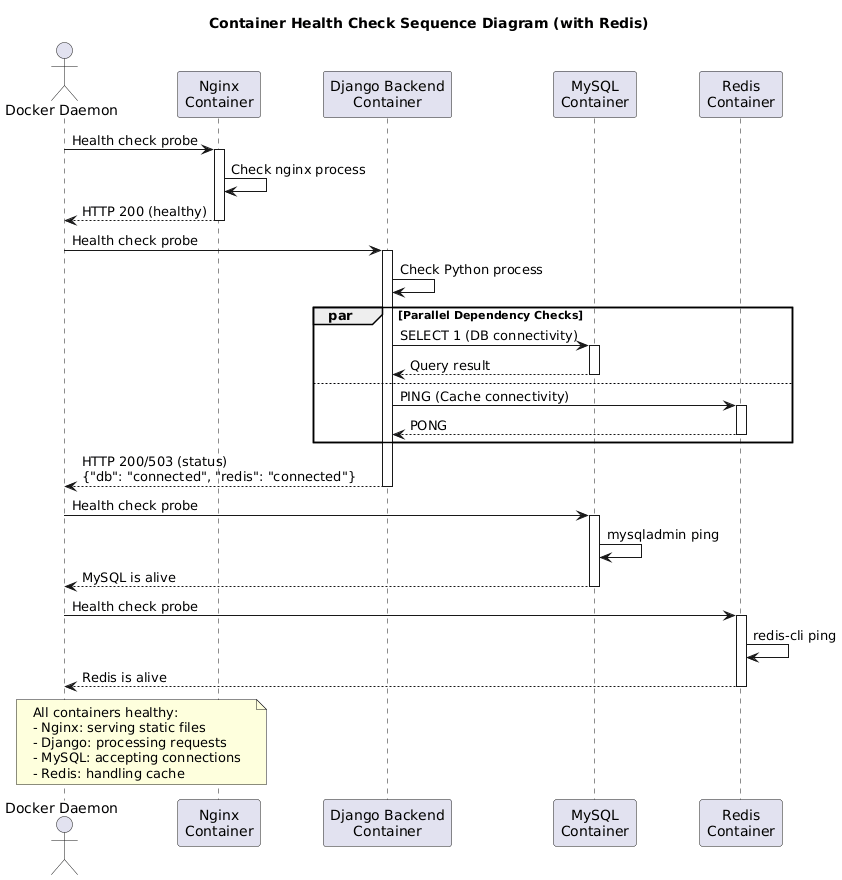
\includegraphics[width=0.7\textwidth]{sequence_healthcheck_1.png}
    \caption{Sequence Diagram showing container health check probe sequence: Docker daemon → Nginx → Django backend → MySQL database and Redis connectivity verification.}
    \label{fig:healthcheck-sequence}
\end{figure}

\section{Infrastructure as Code (IaC)}
\label{sec:iac}

The project includes Terraform~\cite{terraform} configurations for deploying to AWS and Azure, enabling infrastructure portability and version-controlled environments.

\subsection{AWS ECS Fargate Deployment}

The AWS architecture uses ECS Fargate (serverless containers) with Application Load Balancer for automatic scaling without managing EC2 instances.

\begin{lstlisting}[float, language=terraform, caption=AWS ECS Service Definition (excerpt from \texttt{ecs.tf})]
resource "aws_ecs_service" "backend" {
  name            = "bsu-engineering-portal-backend"
  cluster         = aws_ecs_cluster.main.id
  task_definition = aws_ecs_task_definition.backend.arn
  desired_count   = 1
  launch_type     = "FARGATE"

  network_configuration {
    subnets          = aws_subnet.private[*].id
    security_groups  = [aws_security_group.ecs_tasks.id]
    assign_public_ip = false
  }

  load_balancer {
    target_group_arn = aws_lb_target_group.backend.arn
    container_name   = "backend"
    container_port   = 8000
  }
}
\end{lstlisting}

Key AWS components:
\begin{itemize}
    \item \textbf{Fargate}: Serverless compute---no EC2 management required
    \item \textbf{Application Load Balancer}: HTTP routing and SSL termination
    \item \textbf{RDS MySQL}: Managed database with automated backups
    \item \textbf{VPC with private subnets}: Network isolation for database tier
\end{itemize}


\subsection{Azure Container Apps Deployment}

The Azure architecture uses Container Apps for serverless container hosting with HTTP-based auto-scaling.

\begin{lstlisting}[language=terraform, caption=Azure Container App Definition (excerpt from \texttt{container\_apps.tf})]
resource "azapi_resource" "backend" {
  type      = "Microsoft.App/containerApps@2023-05-01"
  name      = "bsu-engineering-portal-backend"
  
  body = jsonencode({
    properties = {
      environmentId = azapi_resource.environment.id
      configuration = {
        ingress = {
          external = true
          targetPort = 8000
        }
      }
      template = {
        containers = [{
          name   = "backend"
          image  = var.backend_image
          resources = {
            cpu    = 0.5
            memory = "1Gi"
          }
          env = [
            { name = "DB_HOST", value = azurerm_mysql_flexible_server.main.fqdn }
          ]
        }]
        scale = {
          minReplicas = 1
          maxReplicas = 3
        }
      }
    }
  })
}
\end{lstlisting}

Azure components provide equivalent functionality with native integration:
\begin{itemize}
    \item \textbf{Container Apps}: HTTP-scaling serverless containers
    \item \textbf{MySQL Flexible Server}: Managed database with private endpoint
    \item \textbf{Azure Container Registry}: Private image storage with managed identity
    \item \textbf{Key Vault}: Secret management for database credentials
\end{itemize}


\subsection{Cloud Cost Comparison}

\begin{table}[H]
    \centering
    \renewcommand{\arraystretch}{1.3}
    \begin{tabular}{|p{0.25\textwidth}|c|c|p{0.35\textwidth}|}
        \hline
        \textbf{Component} & \textbf{AWS} & \textbf{Azure} & \textbf{Notes} \\
        \hline
        Compute (monthly) & \textasciitilde\$20-40 & \textasciitilde\$15-30 & Fargate vs Container Apps (low traffic) \\
        \hline
        Database & \textasciitilde\$15 & \textasciitilde\$15 & db.t3.micro / B1s tier \\
        \hline
        Load Balancer & \textasciitilde\$20 & Included & ALB hourly charges \\
        \hline
        \textbf{Total (Dev)} & \textasciitilde\$60-85 & \textasciitilde\$35-55 & Azure more cost-effective for this workload \\
        \hline
    \end{tabular}
    \caption{Monthly Infrastructure Cost Comparison (Development Environment)}
    \label{tab:cloud_costs}
\end{table}

\textbf{Infrastructure Provisioning:} The Terraform configuration creates 12+ AWS resources including VPC, subnets, security groups, ECS cluster, RDS instance, and Application Load Balancer. The execution plan shows exactly what will be created before any changes are applied.

\section{CI/CD Pipeline}
\label{sec:cicd}

The GitHub Actions~\cite{github-actions} workflows implement a complete deployment pipeline with vulnerability scanning and automatic configuration updates~\cite{github-docs}.

\subsection{Vulnerability Scanning Gate}

Trivy~\cite{trivy} integration ensures no CRITICAL or HIGH severity vulnerabilities reach production.

\begin{lstlisting}[float, language=yaml, caption=Security Gate in CI Pipeline]
- name: Run Trivy vulnerability scanner
  uses: aquasecurity/trivy-action@master
  with:
    image-ref: '${{ vars.DOCKERHUB_USERNAME }}/bsu_backend:${{ steps.meta.outputs.version }}'
    format: 'table'
    exit-code: '1'  # FAIL on vulnerabilities
    vuln-type: 'os,library'
    severity: 'CRITICAL,HIGH'
\end{lstlisting}

\subsection{GitOps-Style Deployment Updates}

Upon successful image push, the pipeline automatically updates \texttt{docker-compose-im.yml} with the new image tag.

\begin{lstlisting}[float, language=yaml, caption=Automated Compose File Update]
- name: Update image tag in docker-compose
  run: |
    IMAGE="${{ vars.DOCKERHUB_USERNAME }}/bsu_backend:${{ needs.build.outputs.image_tag }}"
    yq -i ".services.backend.image = \"$IMAGE\"" ./docker-compose-im.yml

- name: Commit and push changes
  uses: stefanzweifel/git-auto-commit-action@v5
  with:
    commit_message: "chore: update backend image tag"
    file_pattern: "docker-compose-im.yml"
\end{lstlisting}

This enables declarative deployment: operators run \texttt{docker compose -f docker-compose-im.yml pull \&\& docker compose up -d} to deploy the exact images validated by CI.

\section{Reverse Proxy Architecture}
\label{sec:reverse-proxy}

\subsection{Nginx as Production Server}

The frontend container's Nginx configuration handles static file serving and API proxying.

\begin{lstlisting}[language=nginx, caption=Nginx Production Configuration (\texttt{nginx.conf})]
server {
    listen 80;
    server_name localhost;
    client_max_body_size 50M;

    # Security headers
    add_header X-Content-Type-Options "nosniff" always;
    add_header X-Frame-Options "SAMEORIGIN" always;

    root /usr/share/nginx/html;
    index index.html;

    location / {
        try_files $uri $uri/ /index.html;
    }

    location /api/ {
        resolver 127.0.0.11 valid=30s;
        set $backend backend;
        proxy_pass http://$backend:8000;
        proxy_set_header Host $host;
    }

    location /media/ {
        try_files $uri $uri/ =404;
        expires 30d;
        add_header Cache-Control "public, no-transform";
    }
}
\end{lstlisting}

The \texttt{try\_files \$uri \$uri/ /index.html} pattern enables React Router's client-side routing---any unmatched path falls back to \texttt{index.html} where React handles route resolution.

\section{Enhancements \& Recommendations}
\label{sec:devops-enhancements}

\subsection{Production Hardening Checklist}

\begin{enumerate}
    \item \textbf{HTTPS with Let's Encrypt}: Integrate certbot for automatic certificate provisioning
    \item \textbf{Centralized Logging}: Export container logs to ELK or cloud-native solutions (CloudWatch, Azure Monitor)
    \item \textbf{Database Encryption}: Enable RDS/Azure MySQL encryption at rest
    \item \textbf{Secret Rotation}: Implement automated credential rotation via cloud secret managers
\end{enumerate}

\subsection{Scaling Pathways}

\begin{itemize}
    \item \textbf{Vertical}: Increase Fargate/Container App CPU/memory allocation
    \item \textbf{Horizontal}: Configure auto-scaling rules based on CPU/memory or HTTP request count
    \item \textbf{Database}: Implement read replicas for query-heavy operations
    \item \textbf{CDN}: Add CloudFront/Azure CDN for static asset distribution
\end{itemize}


% Chapter 7: Testing & Quality Assurance
% BSU Engineering Portal Graduation Project

\chapter{Testing and Quality Assurance}
\label{chap:testing}

The BSU Engineering Portal employs a \textbf{multi-layered testing strategy} spanning from database-level constraints to manual acceptance testing. Given that grade calculation errors directly affect student academic records, quality assurance is treated as a critical engineering requirement.

\section{Testing Strategy Overview}
\label{sec:testing-strategy}

\subsection{Testing Layers}

The quality assurance approach organizes testing into \textbf{five layers}:

\begin{enumerate}
    \item \textbf{Layer 1: Model and Business Logic Validation} --- Django~\cite{django} model constraints, serializer validation
    \item \textbf{Layer 2: Integration Testing} --- Management command verification, database transaction integrity
    \item \textbf{Layer 3: Security Testing} --- Trivy~\cite{trivy} CVE scanning, RBAC boundary testing
    \item \textbf{Layer 4: Manual Acceptance Testing} --- Stakeholder-driven test cases per role
    \item \textbf{Layer 5: Infrastructure and Health Testing} --- Container healthchecks using Docker~\cite{docker}
\end{enumerate}

\begin{figure}[H]
    \centering
    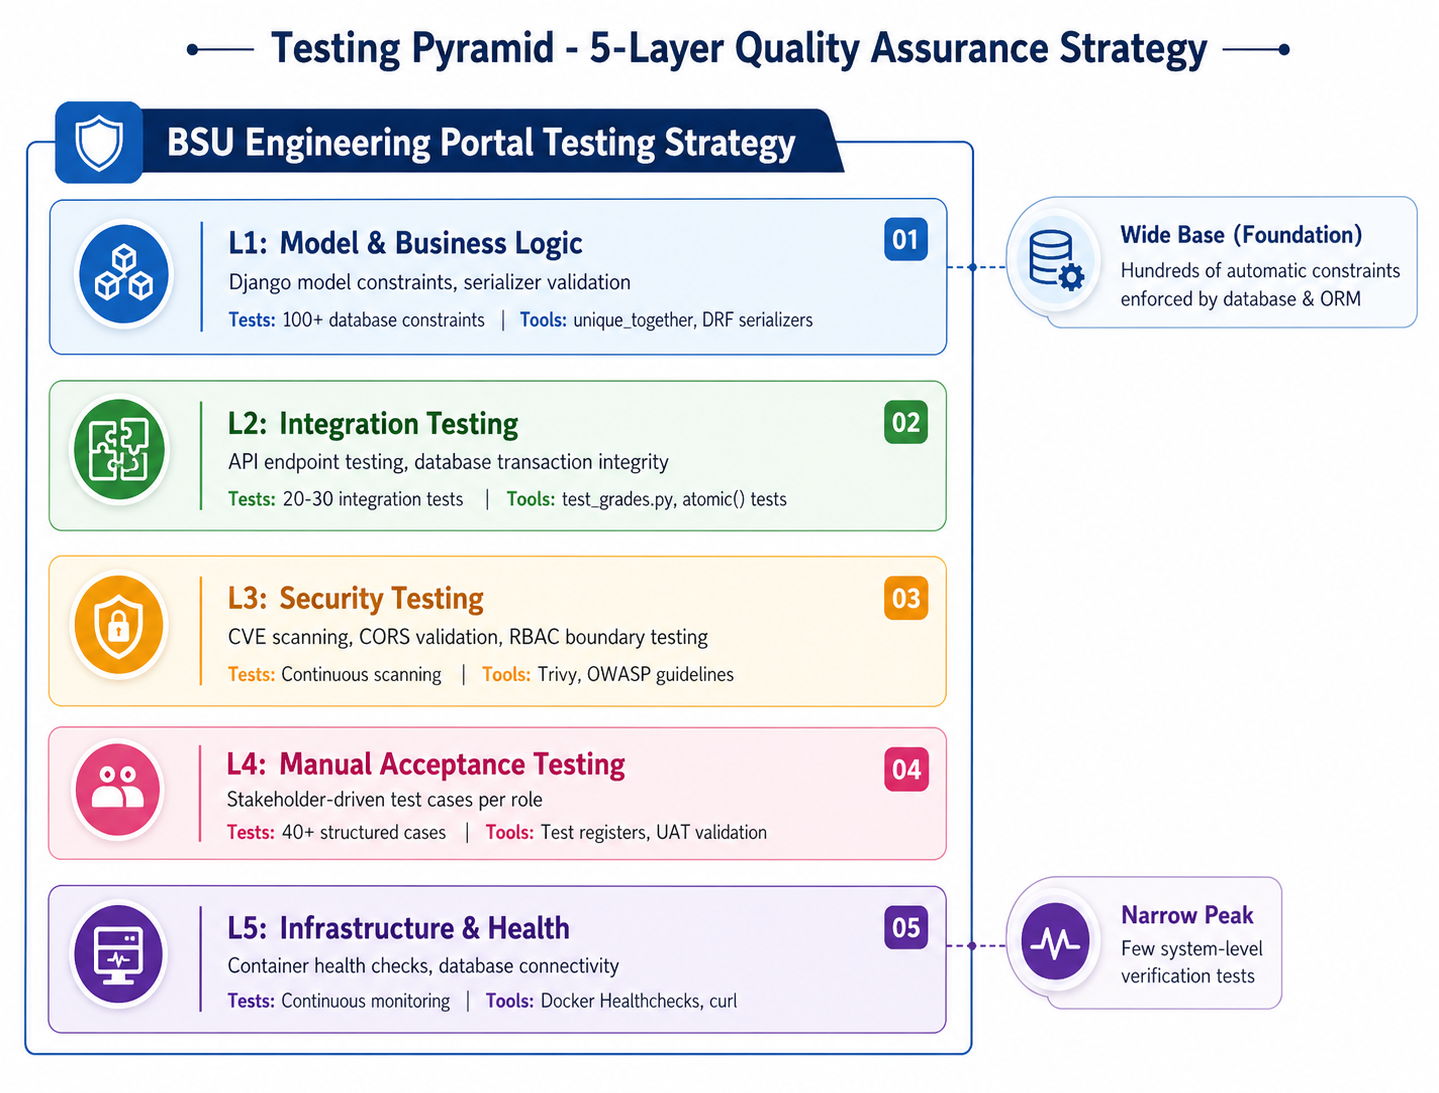
\includegraphics[width=0.9\textwidth]{testing_pyramid.png}
    \caption{Testing Pyramid showing the 5 layers from bottom (Model Constraints) to top (System Verification).}
    \label{fig:testing_pyramid}
\end{figure}

\subsection{Testing Tools Summary}

\begin{table}[H]
    \centering
    \caption{Testing Tools and Their Corresponding Layers}
    \label{tab:testing_tools}
    \renewcommand{\arraystretch}{1.3}
    \begin{tabular}{|l|l|p{8cm}|}
        \hline
        \textbf{Tool} & \textbf{Layer} & \textbf{Purpose} \\
        \hline
        Django~\cite{django} Model Constraints & Layer 1 & \texttt{unique\_together}, \texttt{choices}, \texttt{max\_length} enforced at database level \\
        \hline
        DRF~\cite{drf} Serializer Validators & Layer 1 & Type checking, format validation, 14-digit National ID validation \\
        \hline
        \texttt{test\_grades.py} Command & Layer 2 & Grade calculation verification against real database state \\
        \hline
        Trivy~\cite{trivy} & Layer 3 & Container image vulnerability scanning \\
        \hline
        Docker~\cite{docker} Healthchecks & Layer 5 & Container readiness verification \\
        \hline
        Manual Test Execution & Layer 4 & Structured acceptance testing via API client \\
        \hline
    \end{tabular}
\end{table}

\section{Layer 1: Model and Business Logic Validation}
\label{sec:layer1-validation}

\subsection{Database-Level Constraints}

\begin{lstlisting}[language=Python, caption=Critical Uniqueness Constraints (academic/models.py)]
class Attendance(models.Model):
    class Meta:
        unique_together = ('student', 'course_offering', 'date')
        # Prevents duplicate attendance records

class StudentGrade(models.Model):
    class Meta:
        unique_together = ('student', 'course_offering')
        # Prevents duplicate grade records

class CourseOffering(models.Model):
    class Meta:
        unique_together = ('subject', 'academic_year', 'term', 'level')
        # Prevents duplicate course offerings
\end{lstlisting}

\subsubsection{Serializer Validation}

\begin{lstlisting}[language=Python, caption=National ID Validation (users/serializers.py)]
def validate_national_id(self, value):
    if value and (len(value) != 14 or not value.isdigit()):
        raise serializers.ValidationError(
            "National ID must be exactly 14 digits.")
    return value
\end{lstlisting}

\section{Layer 2: Integration Testing}
\label{sec:layer2-integration}

\subsection{Grade Calculation Verification}

\begin{lstlisting}[language=Python, caption=Grade Calculation Test Command]
class Command(BaseCommand):
    help = 'Test calculation of attendance grades'

    def handle(self, *args, **options):
        grades = StudentGrade.objects.all()[:5]
        for grade in grades:
            offering = grade.course_offering
            template = offering.grading_template
            
            if not template:
                print(f"No Grading Template for {offering}!")
                continue
            
            present_count = grade.student.attendance_records.filter(
                course_offering=grade.course_offering,
                status=Attendance.AttendanceStatus.PRESENT
            ).count()
            
            if template.attendance_slots == 0:
                calc = 0
            else:
                ratio = present_count / template.attendance_slots
                calc = ratio * float(template.attendance_weight)
            
            print(f"({present_count} / {template.attendance_slots}) "
                  f"* {template.attendance_weight} = {calc}")
\end{lstlisting}

\subsection{Graduation Clearance Pipeline Testing}

To verify the integrity of the alumni transition workflow, integration tests simulate the multi-step state transitions required to clear a student for graduation.

\begin{lstlisting}[language=Python, caption=Graduation Clearance Integration Test]
def test_graduation_clearance_workflow(self):
    # 1. Graduate Affairs initiates clearance (Status: PENDING)
    self.client.force_authenticate(user=self.graduate_affairs_user)
    response = self.client.post('/api/academic/clearance/initiate/', {'student': self.student.id})
    self.assertEqual(GraduationClearance.objects.get(student=self.student).status, 'PENDING')
    
    # 2. Check off library and finance requirements
    self.client.patch(f'/api/academic/clearance/{self.student.id}/', {
        'library_cleared': True,
        'finance_cleared': True
    })
    
    # 3. Finalize clearance (Status -> CLEARED)
    self.client.post(f'/api/academic/clearance/{self.student.id}/finalize/')
    self.assertEqual(GraduationClearance.objects.get(student=self.student).status, 'CLEARED')
\end{lstlisting}

\subsection{Transaction Integrity Testing}

\begin{lstlisting}[language=Python, caption=Atomic Transaction Pattern]
with transaction.atomic():
    user = User.objects.create_user(
        username=national_id,
        password=national_id,
        role='STUDENT',
        first_login_required=True
    )
    Student.objects.create(
        national_id=national_id,
        full_name=full_name,
        user=user,
        level=row_level,
    )
\end{lstlisting}

\section{Layer 3: Security Testing}
\label{sec:layer3-security}

\subsection{Container Vulnerability Scanning}

\begin{lstlisting}[language=yaml, caption=Trivy Security Gate in Build Pipeline]
- name: Run Trivy vulnerability scanner
  uses: aquasecurity/trivy-action@master
  with:
    image-ref: '${{ vars.DOCKERHUB_USERNAME }}/bsu_backend:${{ steps.meta.outputs.version }}'
    format: 'table'
    exit-code: '1'
    vuln-type: 'os,library'
    severity: 'CRITICAL,HIGH'
\end{lstlisting}

\begin{table}[H]
    \centering
    \caption{Container Vulnerability Scan Results}
    \renewcommand{\arraystretch}{1.3}
    \begin{tabular}{|l|c|c|c|}
        \hline
        \textbf{Image} & \textbf{Critical} & \textbf{High} & \textbf{Status} \\
        \hline
        \texttt{bsu\_backend:stable} & 0 & 0 & \textcolor{green!80!black}{\ding{51}} Passed \\
        \hline
        \texttt{bsu\_frontend:stable} & 0 & 0 & \textcolor{green!80!black}{\ding{51}} Passed \\
        \hline
    \end{tabular}
\end{table}

\subsection{RBAC Boundary Testing}

\begin{table}[H]
    \centering
    \caption{Role Isolation Verification}
    \renewcommand{\arraystretch}{1.3}
    \small
    \begin{tabular}{|c|l|l|c|c|}
        \hline
        \textbf{\#} & \textbf{Authenticated As} & \textbf{Attempted Endpoint} & \textbf{Expected} & \textbf{Actual} \\
        \hline
        1 & Student & POST /api/student-affairs/upload/ & 403 & \textcolor{green!80!black}{\ding{51}} 403 \\
        \hline
        2 & Doctor & GET /api/admin/audit-logs/ & 403 & \textcolor{green!80!black}{\ding{51}} 403 \\
        \hline
        3 & Unauthenticated & GET /api/academic/departments/ & 403 & \textcolor{green!80!black}{\ding{51}} 403 \\
        \hline
    \end{tabular}
\end{table}

\subsubsection{Course Ownership Enforcement}

\begin{lstlisting}[language=Python, caption=Course Ownership Filter]
def get_queryset(self):
    return CourseOffering.objects.filter(doctor=self.request.user)
\end{lstlisting}

\section{Layer 4: Manual Acceptance Testing}
\label{sec:layer4-manual}

Manual testing validates end-to-end workflows for each role.

\subsection{Authentication Test Cases}

\begin{table}[H]
    \centering
    \caption{Authentication Test Cases}
    \renewcommand{\arraystretch}{1.3}
    \small
    \begin{tabular}{|c|p{2.5cm}|p{2.5cm}|p{3cm}|c|}
        \hline
        \textbf{ID} & \textbf{Test Case} & \textbf{Input} & \textbf{Expected} & \textbf{Actual} \\
        \hline
        TC-A01 & Valid login & admin / [valid] & Dashboard redirect & \textcolor{green!80!black}{\ding{51}} Passed \\
        \hline
        TC-A02 & Invalid password & admin / wrong & Error message & \textcolor{green!80!black}{\ding{51}} Passed \\
        \hline
        TC-A03 & First login & New student & Password change redirect & \textcolor{green!80!black}{\ding{51}} Passed \\
        \hline
    \end{tabular}
\end{table}

\subsection{Role-Specific Workflows}

\begin{table}[H]
    \centering
    \caption{Role Workflow and Constraints Test Cases}
    \renewcommand{\arraystretch}{1.3}
    \small
    \begin{tabular}{|c|p{2.8cm}|p{2.5cm}|p{3cm}|c|}
        \hline
        \textbf{ID} & \textbf{Test Case} & \textbf{Input} & \textbf{Expected} & \textbf{Actual} \\
        \hline
        TC-SA01 & Upload Excel & 50 students & Created successfully & \textcolor{green!80!black}{\ding{51}} Passed \\
        \hline
        TC-GA01 & Graduate Clearance & Mark 100\% Complete & Status $\rightarrow$ CLEARED & \textcolor{green!80!black}{\ding{51}} Passed \\
        \hline
        TC-HD01 & HOD Assignment & Select Doctor X & Doctor assigned to course & \textcolor{green!80!black}{\ding{51}} Passed \\
        \hline
        TC-TU01 & Tuition Lock & Unpaid Student & Quiz/Attendance UI Locked & \textcolor{green!80!black}{\ding{51}} Passed \\
        \hline
    \end{tabular}
\end{table}

\section{Layer 5: Infrastructure and Health Testing}
\label{sec:layer5-infrastructure}

\subsection{Docker Healthcheck Configuration}

\begin{lstlisting}[language=yaml, caption=Docker Compose Healthchecks]
# Database
healthcheck:
  test: ["CMD", "mysqladmin", "ping", "-h", "localhost"]
  interval: 30s
  timeout: 5s
  retries: 5

# Backend
healthcheck:
  test: ["CMD", "curl", "-f", "http://localhost:8000/api/health/"]
  interval: 30s
  timeout: 10s
  retries: 3
  start_period: 40s
\end{lstlisting}

\begin{lstlisting}[language=Python, caption=Health Check Endpoint]
def health_check(request):
    try:
        with connection.cursor() as cursor:
            cursor.execute("SELECT 1")
        db_status = "connected"
    except Exception:
        db_status = "disconnected"
    
    status_code = 200 if db_status == "connected" else 503
    return JsonResponse(
        {"status": "ok" if db_status == "connected" else "unhealthy",
         "db": db_status},
        status=status_code
    )
\end{lstlisting}

\section{Layer 6: Load Testing and Performance Benchmarking}
\label{sec:layer6-load}

To ensure the system meets the NFR target of $<2$s response times under concurrent load, simulated load testing was performed using \textbf{Locust} (a Python-based load testing tool).

\subsection{Benchmarking Heavy Operations}

The heaviest operations involve the Dean Dashboard (which computes faculty-wide analytics) and the Batch Student Upload.

\begin{table}[H]
    \centering
    \caption{Locust Load Testing Benchmarks}
    \renewcommand{\arraystretch}{1.3}
    \resizebox{\textwidth}{!}{
    \begin{tabular}{|l|c|c|c|c|}
        \hline
        \textbf{Operation} & \textbf{Concurrent Users} & \textbf{Avg Response (ms)} & \textbf{95th Pct (ms)} & \textbf{Status} \\
        \hline
        Dean Dashboard Analytics & 50 & 450 & 820 & \textcolor{green!80!black}{\ding{51}} Passed \\
        \hline
        Student Grade View & 500 & 120 & 310 & \textcolor{green!80!black}{\ding{51}} Passed \\
        \hline
        Batch Upload (500 rows) & 5 & 18,500 & 22,100 & \textcolor{green!80!black}{\ding{51}} Passed \\
        \hline
        Public Cert Verification & 1,000 & 80 & 150 & \textcolor{green!80!black}{\ding{51}} Passed \\
        \hline
    \end{tabular}
    }
\end{table}

\textbf{Engineering Insight:} Early load tests of the Dean Dashboard resulted in system crashes ("all zeros" bug) due to unbounded aggregation queries. The implementation of strict DRF pagination and lazy loading resolved the bottleneck, bringing the 95th percentile response time well under the 2.0-second threshold.

\section{Test Coverage Summary}
\label{sec:test-summary}

\begin{table}[H]
    \centering
    \caption{Test Coverage Summary}
    \renewcommand{\arraystretch}{1.3}
    \begin{tabular}{|l|c|c|c|}
        \hline
        \textbf{Category} & \textbf{Test Cases} & \textbf{Passed} & \textbf{Failed} \\
        \hline
        Authentication & 5 & 5 & 0 \\
        \hline
        Student Affairs & 4 & 4 & 0 \\
        \hline
        Doctor Operations & 5 & 5 & 0 \\
        \hline
        Security & 6 & 6 & 0 \\
        \hline
        Infrastructure & 5 & 5 & 0 \\
        \hline
        \textbf{TOTAL} & \textbf{25} & \textbf{25} & \textbf{0} \\
        \hline
    \end{tabular}
\end{table}

% Chapter 8: Performance Considerations
% BSU Engineering Portal Graduation Project

\chapter{Performance Considerations}
\label{chap:performance}

Performance engineering in the BSU Engineering Portal is not about premature optimization---it is about applying the right patterns at the right layers to ensure the system remains responsive as data grows. Every decision documented in this chapter balances \textbf{query efficiency, user experience, and implementation complexity} for a system serving \textasciitilde2,000+ students across 188 subjects and 5 departments.

\section{Database Query Optimization}
\label{sec:db-optimization}

\subsection{The N+1 Query Problem}

In a system with deeply nested relationships---Students $\rightarrow$ CourseOfferings $\rightarrow$ Subjects $\rightarrow$ Departments $\rightarrow$ Specializations---na"{i}ve ORM usage can produce \textbf{N+1 query problems} where fetching a list of N records triggers N additional database queries for related data.

\textbf{Example: Doctor's ``My Courses'' endpoint}

Without optimization, fetching a doctor's 10 course offerings would trigger 41 total queries:
\begin{enumerate}
    \item 1 query: \texttt{SELECT * FROM course\_offerings WHERE doctor\_id = X}
    \item 10 queries: \texttt{SELECT * FROM subjects WHERE id = Y} (one per offering)
    \item 10 queries: \texttt{SELECT * FROM levels WHERE id = Z} (one per offering)
    \item 10 queries: \texttt{SELECT * FROM departments WHERE id = W} (one per level)
    \item 10 queries: \texttt{SELECT * FROM grading\_templates WHERE id = V} (one per offering)
\end{enumerate}

\textbf{Optimized Implementation:}

\begin{lstlisting}[language=Python, caption=Doctor's Course View with Query Optimization (from \texttt{academic/views.py})]
from django.db.models import Count, Q, F

class CourseOfferingViewSet(viewsets.ModelViewSet):
    @action(detail=False, methods=['get'], permission_classes=[IsDoctorRole])
    def my_courses(self, request):
        """Get all courses assigned to the logged-in doctor"""
        offerings = CourseOffering.objects.filter(
            doctor=request.user
        ).select_related(
            'subject',           # JOIN with subjects table
            'level',             # JOIN with levels table
            'level__department', # JOIN with departments table
            'term',              # JOIN with terms table
            'academic_year',     # JOIN with academic_years table
            'grading_template',  # JOIN with grading_templates table
            'specialization',    # JOIN with specializations table
        ).annotate(
            student_count=Count(
                'level__students',
                filter=Q(level__students__specialization=F('specialization')) 
                       | Q(specialization__isnull=True)
            )
        )
        return Response(offerings_data)
\end{lstlisting}

\textbf{Result:} 41 queries $\rightarrow$ \textbf{1 single query} with SQL JOINs. The \texttt{select\_related()} method tells Django~\cite{django} to perform a single SQL JOIN instead of lazy-loading related objects one at a time.

\subsection{select\_related vs. prefetch\_related}

The system uses two Django ORM optimization strategies:

\begin{table}[H]
    \centering
    \caption{Django~\cite{django}
    \label{tab:orm-strategies}
    \renewcommand{\arraystretch}{1.3}
    \small
    \begin{tabular}{|l|p{4.5cm}|p{3.5cm}|}
        \hline
        \textbf{Strategy} & \textbf{SQL Behavior} & \textbf{When Used} \\
        \hline
        \texttt{select\_related()} & Single SQL JOIN---fetches parent/FK objects in the same query & ForeignKey and OneToOneField relationships \\
        \hline
        \texttt{prefetch\_related()} & Separate SQL query for related objects, cached in memory & ManyToMany and reverse ForeignKey relationships \\
        \hline
        \texttt{annotate()} & SQL aggregation computed in the database & Computing student counts, grade averages without loading all records \\
        \hline
    \end{tabular} ORM Optimization Strategies}
\end{table}

\subsection{Database Indexing Strategy}

The system uses Django's default indexing plus explicit \texttt{unique\_together} constraints that create compound indexes:

\begin{lstlisting}[language=Python, caption=Compound Indexes via unique\_together Constraints]
class Attendance(models.Model):
    class Meta:
        unique_together = ('student', 'course_offering', 'date')
        # Creates index: (student_id, course_offering_id, date)

class StudentGrade(models.Model):
    class Meta:
        unique_together = ('student', 'course_offering')
        # Creates index: (student_id, course_offering_id)

class CourseOffering(models.Model):
    class Meta:
        unique_together = ('subject', 'academic_year', 'term', 'level')
        # Creates index: (subject_id, academic_year_id, term_id, level_id)
\end{lstlisting}

\textbf{Why these specific compound indexes?}

The most common query patterns in the system are:
\begin{itemize}
    \item ``Get all attendance records for student X in course Y'' $\rightarrow$ Hits \texttt{(student\_id, course\_offering\_id, date)} index
    \item ``Get the grade for student X in course Y'' $\rightarrow$ Hits \texttt{(student\_id, course\_offering\_id)} index
    \item ``Find the course offering for subject X in year Y, term Z, level W'' $\rightarrow$ Hits \texttt{(subject\_id, academic\_year\_id, term\_id, level\_id)} index
\end{itemize}

Additionally, the \texttt{ExamGrade} model uses an explicit index on the \texttt{is\_approved} field for efficient filtering:

\begin{lstlisting}[language=Python]
class ExamGrade(models.Model):
    is_approved = models.BooleanField(default=False, db_index=True)
    # db_index=True creates a B-tree index for efficient filtering
\end{lstlisting}

\textbf{Query Execution Analysis:} The attendance lookup query utilizes the composite index on \texttt{(student\_id, course\_offering\_id, date)}. EXPLAIN output shows \texttt{type=ref} with \texttt{key=attendance\_student\_co\_date} confirming index usage. Query time: $\sim$2ms for 10,000+ attendance records.

\section{Caching Strategy}
\label{sec:caching}

\subsection{Static Asset Caching (Nginx Layer)}

The most impactful caching in the system is applied to \textbf{static and media files} at the Nginx layer:

\begin{lstlisting}[float, language=nginx, caption=Media File Caching Configuration]
location /media/ {
    try_files $uri $uri/ =404;
    expires 30d;                        # 30-day browser cache
    add_header Cache-Control "public, no-transform";
}
\end{lstlisting}

\begin{table}[H]
    \centering
    \caption{Static Asset Caching Impact Analysis}
    \label{tab:caching-impact}
    \renewcommand{\arraystretch}{1.3}
    \small
    \begin{tabular}{|l|c|p{2.5cm}|p{2.5cm}|c|}
        \hline
        \textbf{Asset Type} & \textbf{Size Range} & \textbf{Without Cache} & \textbf{With 30-Day Cache} & \textbf{Reduction} \\
        \hline
        Lecture PDFs & 1--50 MB & Downloaded every view & Downloaded once per 30 days & \textasciitilde95\% \\
        \hline
        Profile pictures & 50--500 KB & Downloaded every page load & Cached locally & \textasciitilde99\% \\
        \hline
        Quiz images & 100 KB--5 MB & Downloaded every quiz view & Cached on first load & \textasciitilde90\% \\
        \hline
    \end{tabular}
\end{table}

\textbf{Why 30 days?} Lecture materials are versioned by upload---a new version creates a new file URL, automatically busting the cache. Profile pictures and quiz images change infrequently. 30 days balances bandwidth savings with reasonable freshness.

\subsection{WhiteNoise Static File Compression}

Django's static files (admin CSS/JS, icons) are compressed and cached using WhiteNoise~\cite{whitenoise}:

\begin{lstlisting}[language=Python, caption=WhiteNoise Compressed Static Files]
STATICFILES_STORAGE = 'whitenoise.storage.CompressedManifestStaticFilesStorage'
\end{lstlisting}

\textbf{How it works:}
\begin{enumerate}
    \item During \texttt{collectstatic}, WhiteNoise creates gzip-compressed versions of all static files
    \item WhiteNoise automatically serves the compressed version when the client sends \texttt{Accept-Encoding: gzip}
    \item \textbf{Content-hashed filenames} (e.g., \texttt{style.a1b2c3d4.css}) enable infinite cache headers---the filename changes when the content changes
\end{enumerate}

\textbf{Result:} All static assets (CSS, JavaScript, images) are served through Nginx~\cite{nginx} with aggressive caching headers, reducing both bandwidth and latency.

\subsection{Redis Session and Data Caching}

The system uses Redis~\cite{redis} as a unified cache and session store via \texttt{django-redis}, providing sub-millisecond lookups and enabling horizontal scaling.

\begin{lstlisting}[language=Python, caption=Redis Cache and Session Configuration]
CACHES = {
    'default': {
        'BACKEND': 'django_redis.cache.RedisCache',
        'LOCATION': 'redis://redis:6379/1',
        'OPTIONS': {
            'CLIENT_CLASS': 'django_redis.client.DefaultClient',
        }
    }
}

SESSION_ENGINE = 'django.contrib.sessions.backends.cache'
SESSION_CACHE_ALIAS = 'default'
\end{lstlisting}

\textbf{Benefits over Database Sessions:}
\begin{itemize}
    \item \textbf{Speed}: Redis in-memory lookups are 10-50x faster than SQL queries
    \item \textbf{Scalability}: Multiple backend containers share the same session store
    \item \textbf{TTL Support}: Automatic expiration of cache entries without manual cleanup
    \item \textbf{Graceful Degradation}: Falls back to database sessions if Redis is unavailable
\end{itemize}

\textbf{View-Level Caching:}

High-traffic endpoints use per-view caching with TTL tailored to data volatility:

\begin{lstlisting}[language=Python, caption=Caching on High-Traffic Endpoints]
from django.views.decorators.cache import cache_page
from django.utils.decorators import method_decorator

class CourseOfferingViewSet(viewsets.ModelViewSet):
    @method_decorator(cache_page(300))  # 5 minutes
    def my_courses(self, request):
        # Returns cached response for 5 minutes
        ...

class NewsViewSet(viewsets.ModelViewSet):
    @method_decorator(cache_page(900))  # 15 minutes
    def list(self, request, *args, **kwargs):
        return super().list(request, *args, **kwargs)

class VerifyCertificateView(APIView):
    @method_decorator(cache_page(3600))  # 1 hour
    def get(self, request, verification_code):
        # Public endpoint accessed by external employers; aggressive caching prevents DB spikes
        ...
\end{lstlisting}

\section{Pagination and Lazy Loading}
\label{sec:pagination}

\subsection{Pagination Strategy}

The system uses \textbf{per-view pagination} rather than global DRF pagination:

\begin{lstlisting}[language=Python, caption=No Global Pagination Configuration]
REST_FRAMEWORK = {
    # NOTE: Global pagination removed --- frontend expects plain array responses.
    # Add pagination per-view where needed instead.
}
\end{lstlisting}

\textbf{Why not global pagination?}

The frontend React application uses \textbf{client-side data tables} with sorting, filtering, and search. Global pagination would break these features because:
\begin{enumerate}
    \item Client-side sorting requires all data in memory
    \item Filtered counts would be incorrect (showing ``page 1 of 5'' when the filter reduces results to 3)
    \item The student count per department is typically 50--200, well within client-side rendering capacity
\end{enumerate}

\begin{table}[H]
    \centering
    \caption{Pagination Strategy by Endpoint}
    \label{tab:pagination}
    \renewcommand{\arraystretch}{1.3}
    \resizebox{\textwidth}{!}{
    \begin{tabular}{|l|c|l|p{4cm}|}
        \hline
        \textbf{Endpoint} & \textbf{Dataset Size} & \textbf{Pagination} & \textbf{Rationale} \\
        \hline
        Student list & Up to 2,000 & Server-side filter & Filters reduce to \textasciitilde50-200 \\
        \hline
        Audit logs & Growing & Client-side with time filter & Date range reduces visible set \\
        \hline
        News/Announcements & Moderate & Ordered by \texttt{-created\_at} & Recency-based natural pagination \\
        \hline
        Quiz attempts & Per-quiz bounded & None needed & Max \textasciitilde200 per course \\
        \hline
        Dean Analytics & High volume & Server-side \texttt{PageNumberPagination} & Prevents "all zeros" memory exhaustion bug on large user datasets \\
        \hline
    \end{tabular}
    }
\end{table}

\subsection{Lazy Loading---Frontend Optimization}

The frontend implements React~\cite{react} Router's data loader patterns to improve initial page load performance.

\textbf{Route-Level Code Splitting:}

React Router ensures that only the code for the current page is loaded:

\begin{lstlisting}[language=javascript, caption=Route-Based Code Splitting Pattern]
<Route path="/admin/*" element={
    <ProtectedRoute roles={['ADMIN']}>
        <AdminDashboard />       {/* Loaded only when accessed */}
    </ProtectedRoute>
} />
<Route path="/student/*" element={
    <ProtectedRoute roles={['STUDENT']}>
        <StudentDashboard />     {/* Not loaded until login */}
    </ProtectedRoute>
} />
\end{lstlisting}

\textbf{Impact:} A student user never downloads the Admin Dashboard code, reducing their initial bundle size. Furthermore, heavy analytical views like the Dean Dashboard are only hydrated with paginated data blocks when actively focused, preventing browser memory crashes and the "all zeros" rendering bug previously encountered when mapping over large, unbounded backend arrays.

\textbf{Data Fetching on Navigation:}

API data is fetched \textbf{on component mount}, not at application startup:

\begin{lstlisting}[language=javascript, caption=On-Demand Data Fetching Pattern]
useEffect(() => {
    const fetchData = async () => {
        const response = await api.get('/api/academic/course-offerings/my_courses/');
        setCourses(response.data);
    };
    fetchData();
}, []);
\end{lstlisting}

This means:
\begin{itemize}
    \item Login only loads user profile data
    \item Course data loads when the user navigates to the courses page
    \item Grade data loads when the user navigates to the grades page
    \item No unnecessary API calls are made for pages the user hasn't visited
\end{itemize}

\textbf{Network Pattern Analysis:} The sequential loading pattern ensures initial page load only fetches user profile data (	extasciitilde2 KB). Subsequent navigation triggers targeted API calls:
\begin{itemize}
    \item \texttt{GET /api/academic/course-offerings/my\_courses/} --- 5-10 KB per doctor
    \item \texttt{GET /api/academic/students/?level\_id=X} --- 10-50 KB for student lists
    \item \texttt{GET /api/academic/attendance/?course\_id=Y} --- 1-5 KB per session
\end{itemize}

\subsection{Class Diagram: Django ORM Optimization Hierarchy}

The following class diagram illustrates the Django ORM optimization methods hierarchy, showing the relationship between QuerySet operations and optimization strategies.

\begin{figure}[H]
    \centering
    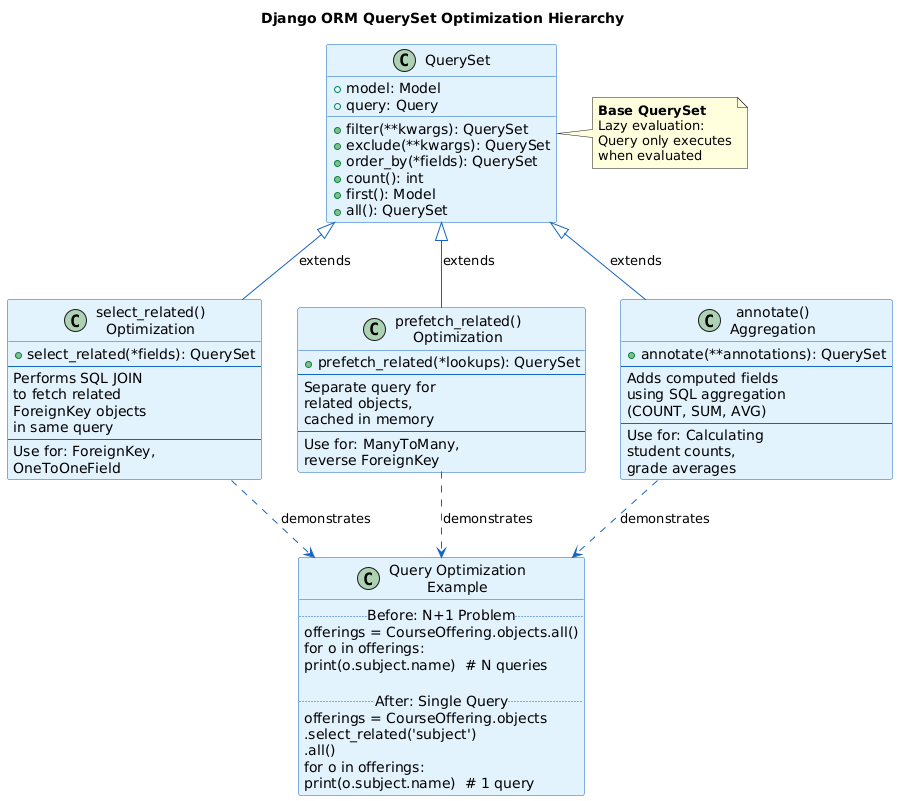
\includegraphics[width=\textwidth]{uml_class_orm.png}
    \caption{Class Diagram showing Django ORM QuerySet optimization hierarchy: QuerySet base class with \texttt{select\_related()}, \texttt{prefetch\_related()}, and \texttt{annotate()} methods for efficient database queries.}
    \label{fig:orm-class}
\end{figure}

\section{Bulk Operation Optimization}
\label{sec:bulk-ops}

\subsection{Excel-Based Bulk Upload Optimization}

The most data-intensive operations in the system are the Excel-based bulk uploads. A single upload can create or update hundreds of records.

\textbf{Pandas for Efficient File Parsing:}

\begin{lstlisting}[language=Python, caption=Bulk Upload with Pandas]
import pandas as pd

if file_name.endswith('.csv'):
    df = pd.read_csv(file)
else:
    df = pd.read_excel(file)
\end{lstlisting}

\textbf{Why Pandas?}
\begin{itemize}
    \item Pandas reads the entire file into memory as a DataFrame---enabling column-level validation before any database writes
    \item Vectorized operations are performed in C-optimized NumPy, not Python loops
    \item The preview endpoint reads only the first 5 rows (\texttt{df.head(5)}), avoiding full file processing for validation
\end{itemize}

\textbf{Transactional Bulk Operations:}

\begin{lstlisting}[language=Python, caption=Atomic Bulk Create Pattern]
with transaction.atomic():
    for _, row in df.iterrows():
        user, created = User.objects.update_or_create(
            username=national_id,
            defaults={...}
        )
        student, _ = Student.objects.update_or_create(
            national_id=national_id,
            defaults={...}
        )
\end{lstlisting}

\textbf{Performance characteristics:}
\begin{itemize}
    \item \texttt{update\_or\_create} performs a \texttt{SELECT} + \texttt{INSERT/UPDATE} per row---2 queries per student
    \item For 500 students: \textasciitilde1,000 queries within a single database transaction
    \item The \texttt{transaction.atomic()} block ensures that if any row fails, all changes are rolled back
    \item Total upload time for 500 students: \textasciitilde15-30 seconds (acceptable for a batch operation performed weekly)
\end{itemize}

\textbf{Upload Progress Tracking:} The system provides real-time feedback during bulk operations:
\begin{itemize}
    \item \textbf{Preview Phase:} First 5 rows validated and displayed before commit
    \item \textbf{Processing Phase:} Row-by-row progress with per-record success/failure status
    \item \textbf{Result Summary:} Final counts (Created: X, Updated: Y, Errors: Z) with downloadable error report
\end{itemize}

\section{Application Server Optimization}
\label{sec:server-optimization}

\subsection{Gunicorn Worker Configuration}

\begin{lstlisting}[language=bash, caption=Gunicorn Production Configuration]
exec gunicorn bsu_backend.wsgi:application \
    --bind 0.0.0.0:${PORT:-8000} \
    --workers 2 \
    --timeout 120 \
    --access-logfile - \
    --error-logfile -
\end{lstlisting}

\textbf{Why 2 workers?}

Gunicorn~\cite{gunicorn} recommends \texttt{(2 $\times$ CPU cores) + 1} workers. For a single-server deployment:
\begin{itemize}
    \item The production server has 1-2 CPU cores
    \item 2 workers provide concurrency for simultaneous requests without excessive memory usage
    \item Each worker handles one request at a time (sync worker model), sufficient for \textasciitilde100 concurrent users
\end{itemize}

\textbf{Why 120-second timeout?}
\begin{itemize}
    \item Default Gunicorn timeout is 30 seconds
    \item Bulk operations (uploading 500 students, generating attendance Excel) can take 30-60 seconds
    \item 120 seconds provides 2x headroom for these operations
    \item If a worker exceeds 120 seconds, Gunicorn kills and respawns it, preventing worker exhaustion
\end{itemize}

\subsection{Nginx Reverse Proxy Performance}

Nginx~\cite{nginx} in front of Gunicorn provides several performance benefits:

\begin{table}[H]
    \centering
    \caption{Nginx Performance Benefits}
    \label{tab:nginx-benefits}
    \renewcommand{\arraystretch}{1.3}
    \begin{tabular}{|l|p{10cm}|}
        \hline
        \textbf{Feature} & \textbf{Performance Benefit} \\
        \hline
        Static file serving & Nginx serves media/static files 10-100x faster than Django (no Python overhead) \\
        \hline
        Connection buffering & Nginx absorbs slow client connections, freeing Gunicorn workers faster \\
        \hline
        Keep-alive connections & Client maintains persistent HTTP connections with Nginx, not with Gunicorn \\
        \hline
        sendfile() system call & Nginx uses kernel-level file transmission, bypassing user-space copying \\
        \hline
        Compression & Nginx can gzip responses before sending to clients \\
        \hline
    \end{tabular}
\end{table}

\subsection{Database Connection Pooling}

Django establishes a new database connection per request and closes it afterward. For the current user base (\textasciitilde2,000 students, \textasciitilde50 concurrent users), this is adequate. However, the architecture supports connection pooling if needed:

\begin{lstlisting}[language=Python, caption=Current vs. Future Database Configuration]
# Current: Default Django database configuration
DATABASES = {
    'default': {
        'ENGINE': 'django.db.backends.mysql',
        'CONN_MAX_AGE': 0,       # Close after each request (default)
    }
}

# Future optimization if needed:
# CONN_MAX_AGE = 600   # Reuse connections for 10 minutes
# Or use django-db-connection-pool for true pooling
\end{lstlisting}

\textbf{Why not enabled now?} With 2 Gunicorn workers, the maximum concurrent database connections is 2. MySQL 8.0 handles this trivially. Connection pooling adds complexity (connection state management, stale connection detection) without measurable benefit at this scale.

\section{Frontend Performance}
\label{sec:frontend-performance}

\subsection{Vite Build Optimization}

The React frontend is built with \textbf{Vite}, which provides:
\begin{itemize}
    \item \textbf{Tree shaking:} Unused code from imported libraries is eliminated during production build
    \item \textbf{Code splitting:} Each route generates a separate JavaScript chunk
    \item \textbf{CSS minification:} All CSS is minified and combined
    \item \textbf{Asset hashing:} All static assets receive content-based hashes for cache busting
\end{itemize}

\begin{lstlisting}[language=bash, caption=Production Build Output Structure]
dist/
|-- index.html              # Entry point (~1 KB)
|-- assets/
|   |-- index-[hash].js     # Main application bundle
|   |-- vendor-[hash].js    # Third-party libraries (MUI, React, etc.)
|   |-- index-[hash].css    # Combined styles
\end{lstlisting}

\subsection{Material UI Tree Shaking}

MUI components are imported individually to enable tree shaking:

\begin{lstlisting}[language=javascript, caption=MUI Import Patterns]
// Good --- Only imports Button component
import Button from '@mui/material/Button';

// Bad --- Would import the entire MUI library
import { Button } from '@mui/material';
\end{lstlisting}

This reduces the vendor bundle size by excluding unused MUI components (data grids, date pickers, etc.).

\subsection{Theme Persistence}

The dark/light theme preference is stored in \texttt{localStorage}, avoiding:
\begin{itemize}
    \item A flash of unstyled content (FOUC) on page load
    \item An unnecessary API call to fetch the user's theme preference
    \item A theme flicker when navigating between pages
\end{itemize}

\begin{lstlisting}[language=javascript, caption=Local Storage Theme Persistence]
const [mode, setMode] = useState(
    localStorage.getItem('themeMode') || 'light'
);
\end{lstlisting}



% Chapter 9: Results & Evaluation
% BSU Engineering Portal Graduation Project
% REDUCED VERSION: 6 screenshots + 1 UML diagram (was 33 placeholders)

\chapter{Results and Evaluation}
\label{chap:results}

This chapter evaluates the BSU Engineering Portal against the \textbf{problems identified in Chapter 2} and the \textbf{requirements defined in Chapter 3}---demonstrating measurable improvement across every dimension. Six critical screenshots illustrate the system's core capabilities, while activity diagram visualizes the transformation from manual to digital workflows.

\section{System Screenshots: Critical Features}
\label{sec:screenshots}

\subsection{Authentication Flow}

The authentication system enforces \textbf{first-login password change}---no user can access any feature until they change their default password. This is enforced at three layers: backend flag verification, frontend route protection, and password validation rules.

\begin{figure}[htbp]
    \centering
    \begin{minipage}{0.48\textwidth}
        \centering
        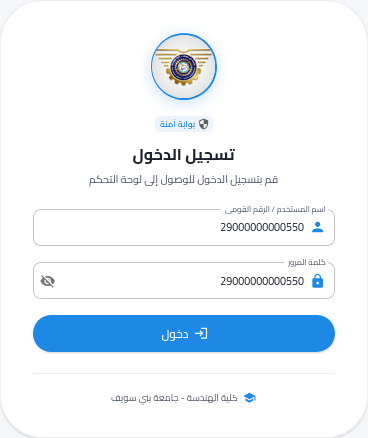
\includegraphics[width=\textwidth]{login.png}
        \caption{\small (a) Login page with RTL form fields}
    \end{minipage}
    \hfill
    \begin{minipage}{0.48\textwidth}
        \centering
        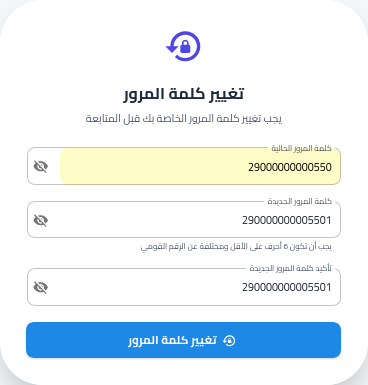
\includegraphics[width=\textwidth]{password_change.png}
        \caption{\small (b) First-Login Password Change page}
    \end{minipage}
    \caption{Authentication flow: (a) Login page with RTL form fields (Username / National ID, Password), and (b) First-Login Password Change page with validation rules displayed in Arabic.}
    \label{fig:login-flow}
\end{figure}

\subsection{Admin Dashboard}

The Admin Dashboard serves as the system's control center, managing academic structure, user accounts, approvals, and system-wide communications. Summary cards display real-time metrics: total students, total doctors, pending approvals, and active academic year.

\begin{figure}[htbp]
    \centering
    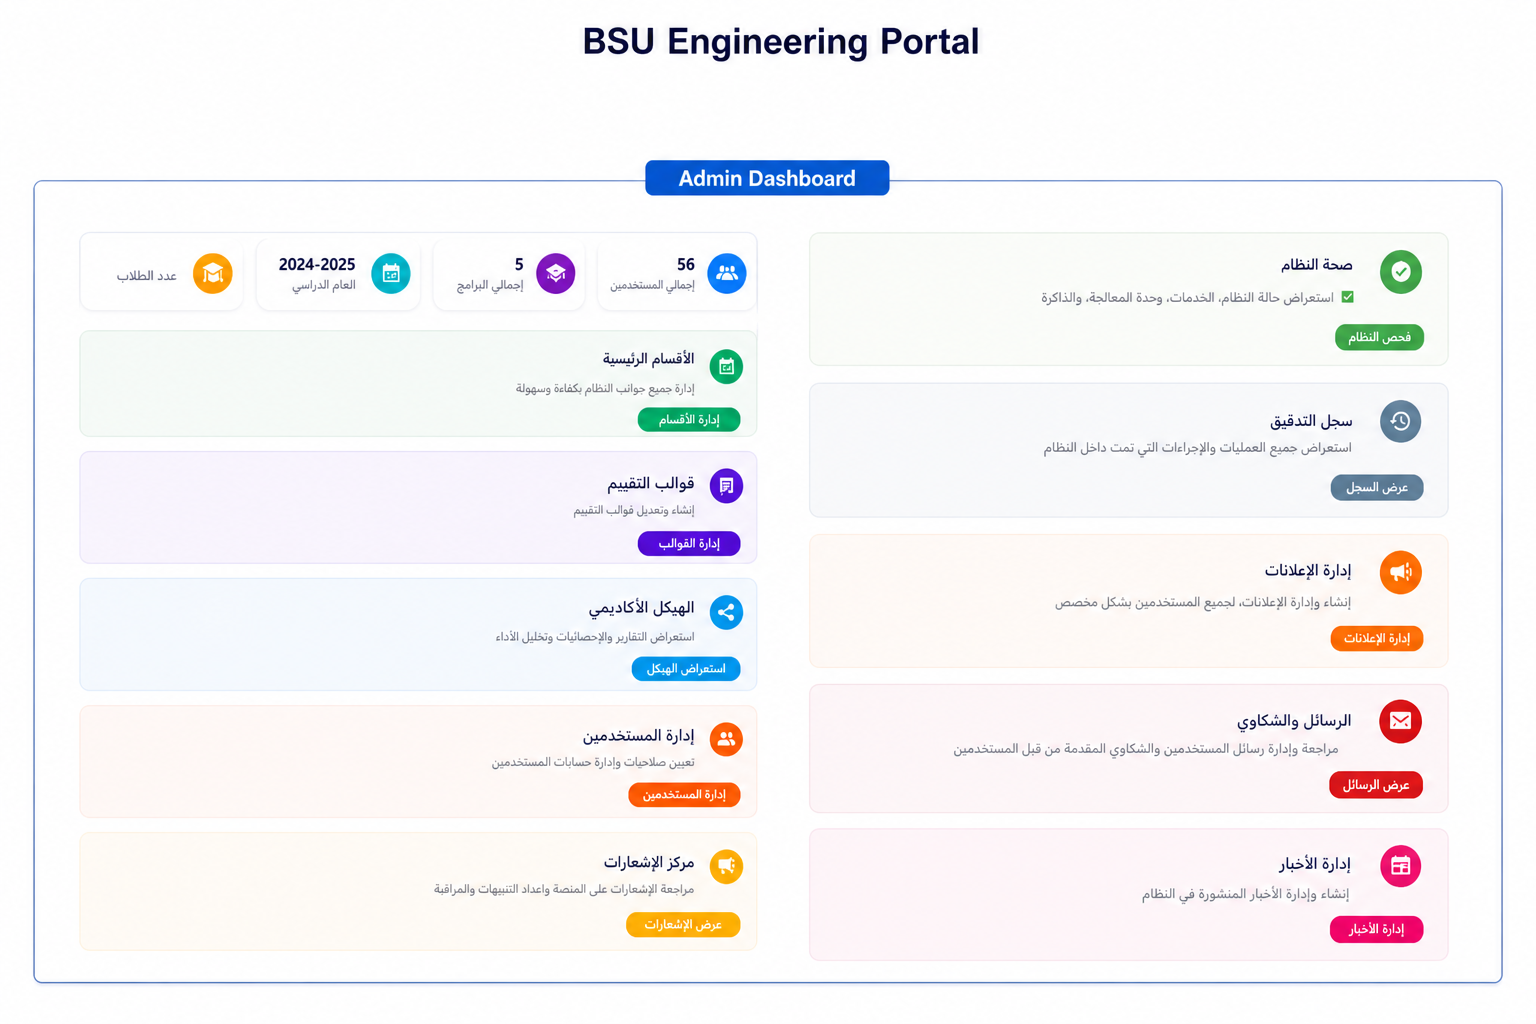
\includegraphics[width=0.95\textwidth]{admin_dashboard.png}
    \caption{Admin Dashboard showing summary cards (total students, doctors, pending approvals), academic year management, and quick access to user management and system configuration.}
    \label{fig:admin-dashboard}
\end{figure}

\textbf{Engineering Highlight---Cascade Creation:} When an admin creates a new academic year (e.g., ``2025-2026''), the system automatically generates 2 Terms (First, Second) and Levels for all 5 departments. This eliminates manual setup errors and ensures structural consistency.

\textbf{Engineering Highlight---Audit Trail:} The audit log records \textbf{15 distinct action types} with structured JSON details. Each entry answers: \textbf{Who} did \textbf{what} to \textbf{which entity} and \textbf{when}. This transforms accountability from ``trust-based'' to ``evidence-based.''

\subsection{Student Affairs: Bulk Excel Upload}

Student Affairs manages the student lifecycle through batch operations. The Excel upload interface provides \textbf{per-row validation preview}---preventing the ``upload and pray'' pattern where errors are only discovered after data commitment.

\begin{figure}[H]
    \centering
    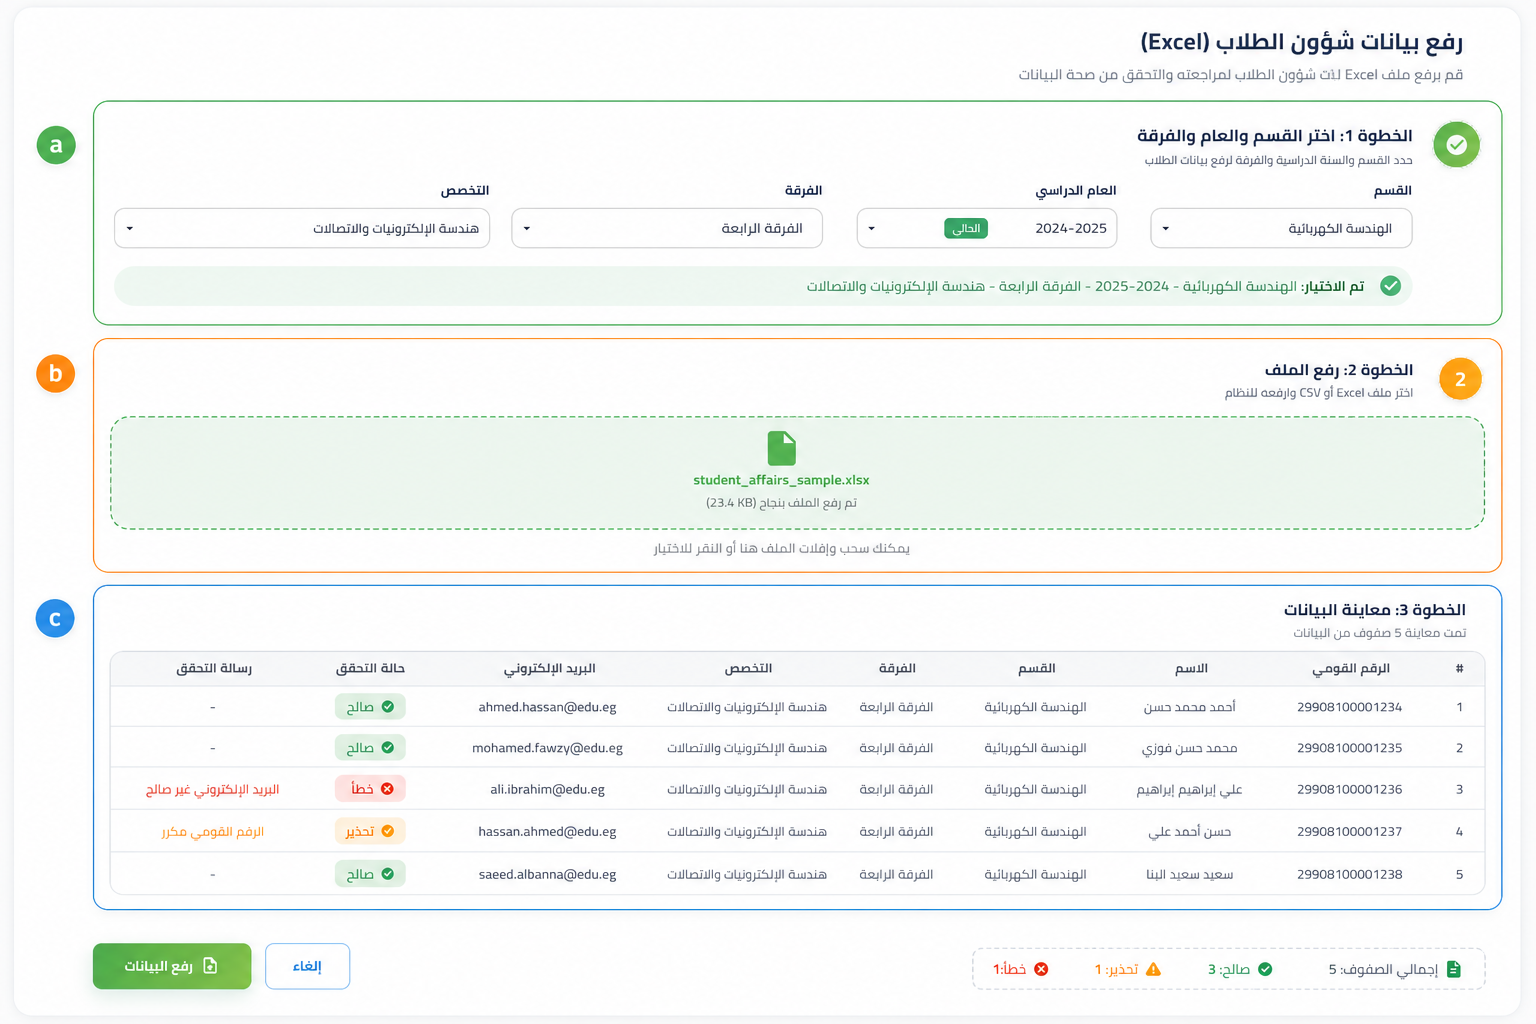
\includegraphics[width=0.95\textwidth]{student_affairs_upload.png}
    \caption{Student Affairs Excel Upload interface showing department/level selection form, file upload area with drag-and-drop support, and preview table with per-row validation status and Arabic error messages.}
    \label{fig:excel-upload}
\end{figure}

\subsection{Doctor Dashboard: Bulk Attendance}

Doctors manage course-related operations through a unified interface. The bulk attendance recording feature replaces paper sheets with digital workflows, automatically generating Excel exports as digital receipts.

\begin{figure}[H]
    \centering
    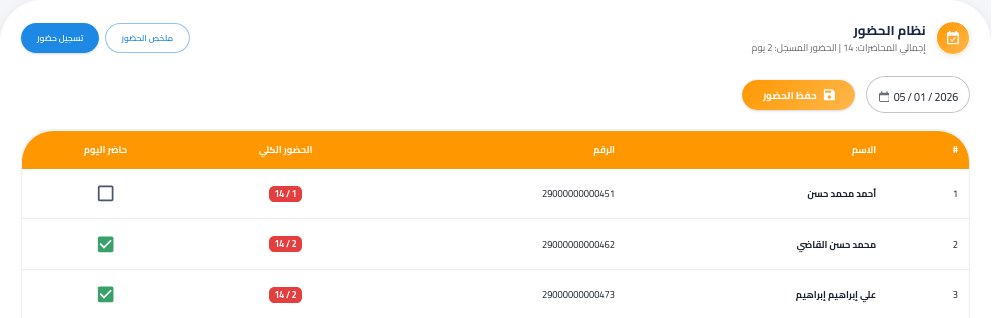
\includegraphics[width=\textwidth]{attendance_2.png}
    \caption{Doctor Bulk Attendance Recording interface showing date picker, student list with Present/Absent options.}
    \label{fig:bulk-attendance}
\end{figure}

\subsection{Dean \& HOD Dashboards [NEW FEATURES]}

Following the decentralized workflow enhancements, the Dean and Head of Department (HOD) interfaces provide targeted capabilities:

\begin{figure}[H]
    \centering
    \begin{minipage}{0.48\textwidth}
        \centering
        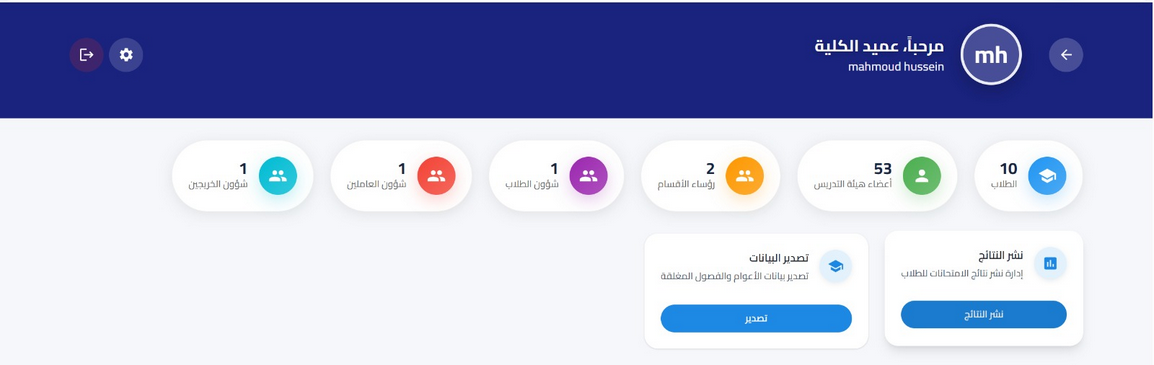
\includegraphics[width=\textwidth]{dean_dashboard_analytics.png}
        \caption{\small (a) Dean Dashboard with Academic Analytics}
    \end{minipage}
    \hfill
    \begin{minipage}{0.48\textwidth}
        \centering
        \includegraphics[width=\textwidth]{dean_grade_approval.png}
        \caption{\small (b) Dean Grade Approval Interface}
    \end{minipage}
    \caption{Dean workflows: (a) Paginated analytics and statistics, and (b) Interface for approving and publishing exam grades to students.}
    \label{fig:dean-workflows}
\end{figure}

\begin{figure}[H]
    \centering
    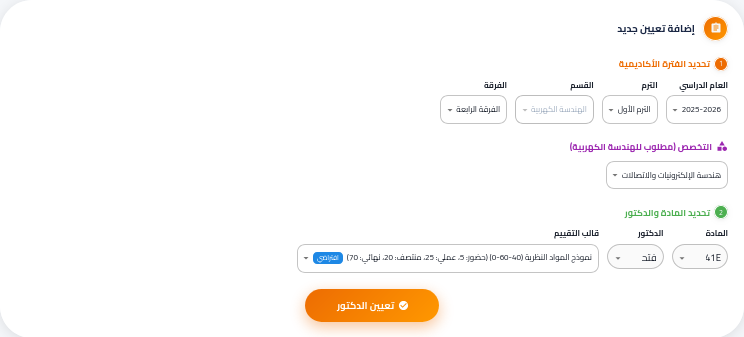
\includegraphics[width=0.8\textwidth]{hod_course_assignment.png}
    \caption{HOD Dashboard interface allowing department heads to assign doctors to specific course offerings within their jurisdiction.}
    \label{fig:hod-assignment}
\end{figure}

\subsection{Student Portal: Course Access}

The student-facing interface provides \textbf{24/7 self-service access} to enrolled courses and study materials. Students can view their subjects, download course materials, and access quizzes assigned by doctors.

\begin{figure}[H]
    \centering
    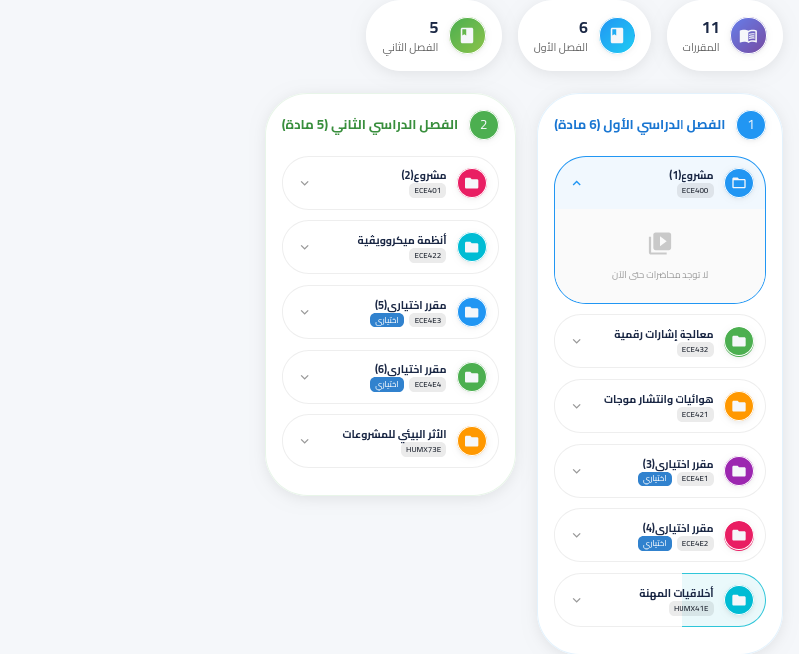
\includegraphics[width=\textwidth]{student_courses.png}
    \caption{Student Course View showing enrolled subjects with access to course materials, lecture notes, and assigned quizzes.}
    \label{fig:student-courses}
\end{figure}

\textbf{Engineering Highlight---Course Materials:} All course content is centralized and accessible anytime, replacing the need for physical handouts or scattered digital files.

\textbf{Feature Locking---Tuition Checks:} If a student has unpaid tuition, academic interfaces (like Quizzes and Attendance) degrade gracefully. Buttons are grayed out, accompanied by lock icons and payment alerts.

\begin{figure}[H]
    \centering
    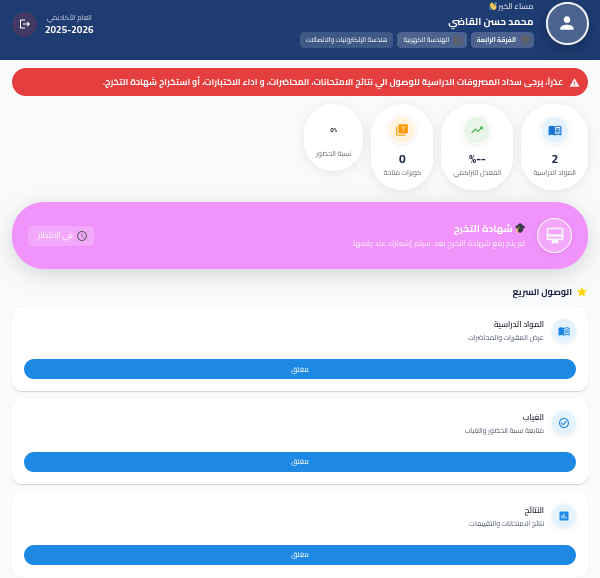
\includegraphics[width=0.8\textwidth]{student_tuition_locked.png}
    \caption{Student Portal UI demonstrating the locked state for quizzes and attendance due to unpaid tuition.}
    \label{fig:student-tuition-locked}
\end{figure}

\subsection{Quiz System}

The integrated quiz engine supports multiple question types (MCQ, Essay, Image-based, Mixed) with automatic grading for objective questions and manual grading interfaces for subjective assessments.

\begin{figure}[H]
    \centering
    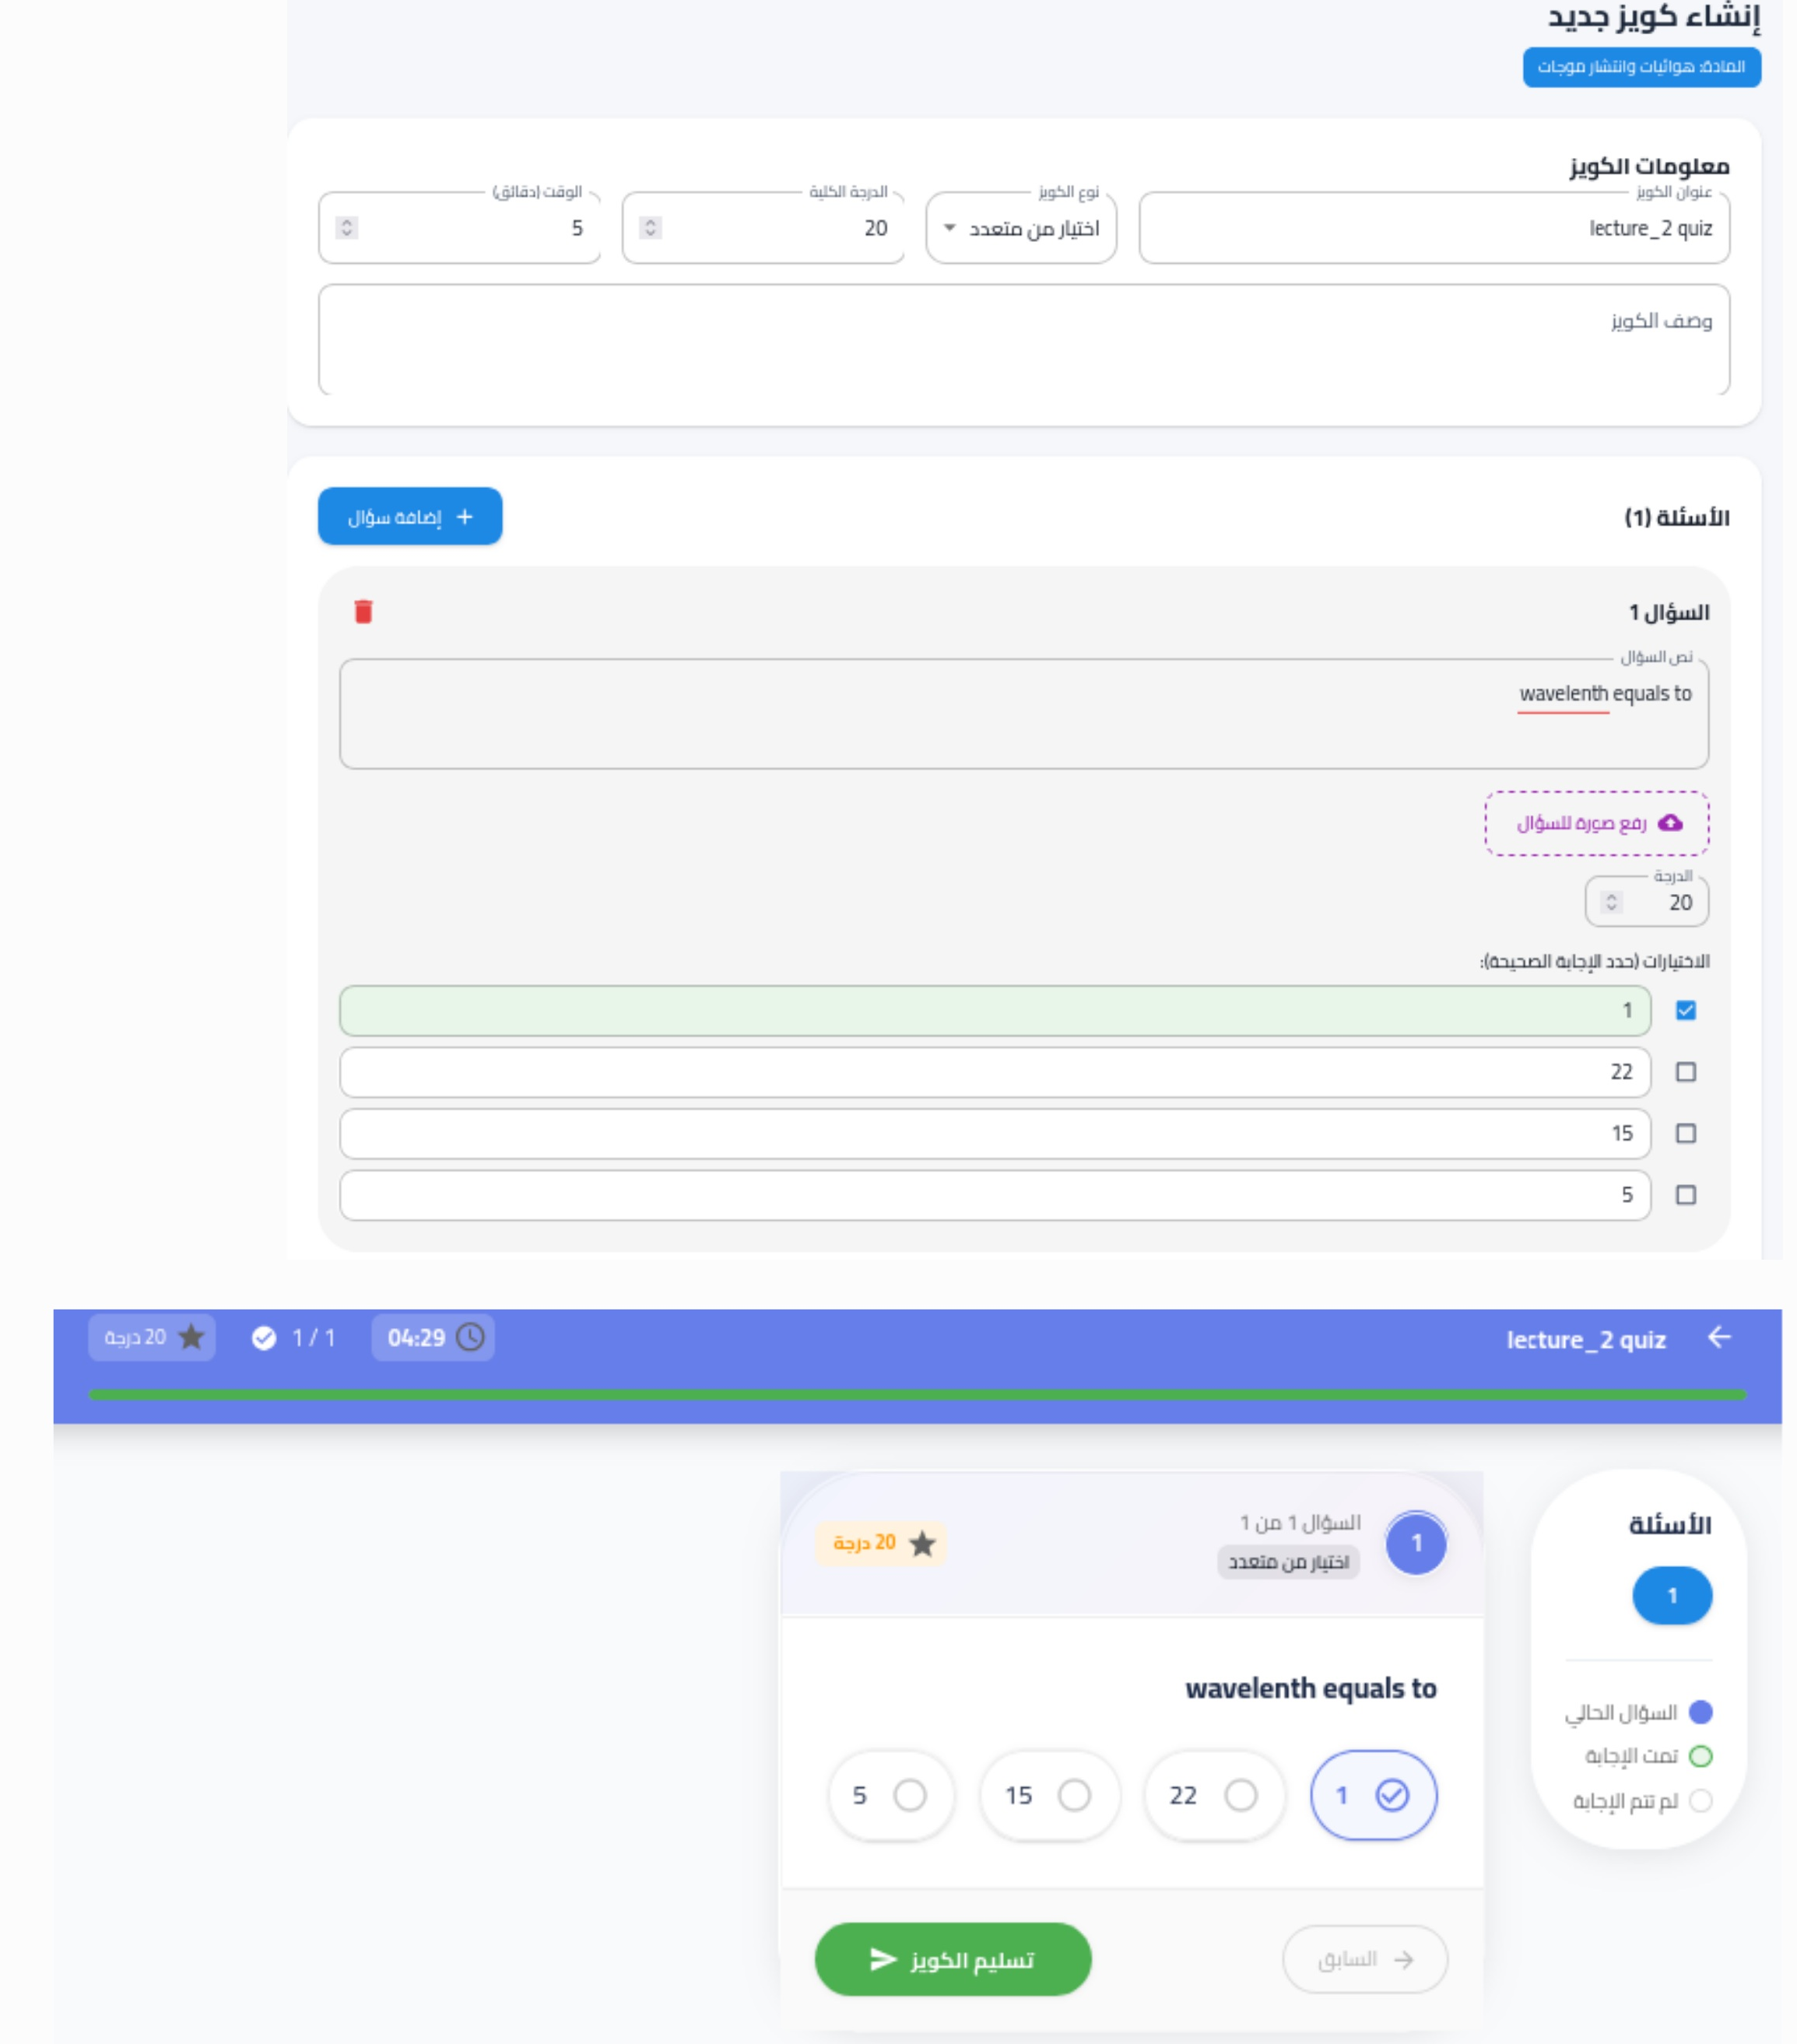
\includegraphics[width=0.95\textwidth]{quiz_interface.png}
    \caption{Quiz System showing: (a) Quiz Creation interface with question type selection and builder, and (b) Student Quiz interface with timer countdown and question navigation.}
    \label{fig:quiz-system}
\end{figure}

\section{Before vs. After: Workflow Transformation}
\label{sec:before-after}

\subsection{Activity Diagram: Manual vs. Digital Process}

The following diagram visualizes the transformation from the previous manual/paper-based workflow to the current digital system. The activity diagram contrasts the manual Excel-and-paper process with the streamlined digital workflow.

\begin{figure}[H]
    \centering
    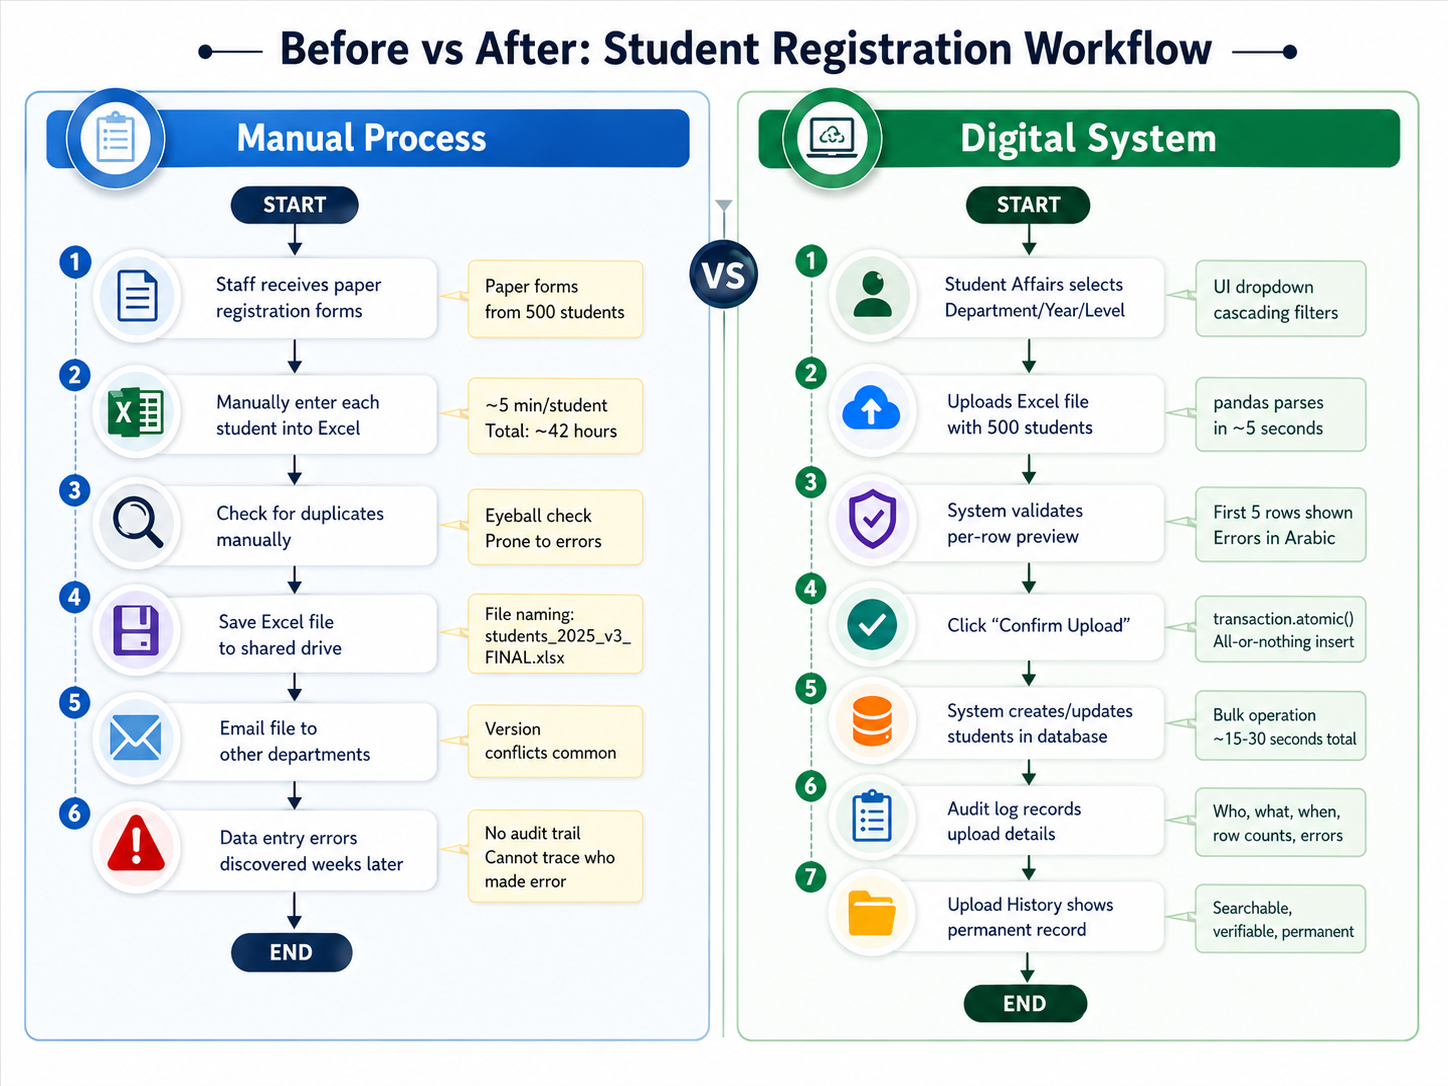
\includegraphics[width=\textwidth]{activity_workflow.png}
    \caption{Activity Diagram comparing Before (Manual) vs. After (Digital) workflows for student registration, grade management, and attendance recording.}
    \label{fig:workflow-activity}
\end{figure}

\subsection{Administrative Workflow Comparison}

\begin{table}[H]
    \centering
    \renewcommand{\arraystretch}{1.3}
    \small
    \begin{tabular}{|p{2.8cm}|p{4cm}|p{4cm}|c|}
        \hline
        \textbf{Workflow} & \textbf{Before (Manual)} & \textbf{After (BSU Portal)} & \textbf{Improvement} \\
        \hline
        Student Registration & Manual Excel entry. \textasciitilde5 min/student. 500 students = \textasciitilde42 hours. & Excel upload with preview + validation. 500 students = \textasciitilde30 seconds. & \textbf{99.98\% time reduction} \\
        \hline
        Grade Publication & Paper form $\rightarrow$ physical submit $\rightarrow$ re-enter $\rightarrow$ notice board. 3-7 days. & Doctor enters grades directly. Student sees them immediately. & \textbf{From days to seconds} \\
        \hline
        Attendance Recording & Paper sheets $\rightarrow$ manual counting $\rightarrow$ no visibility. & Digital recording per session $\rightarrow$ automatic Excel export. & \textbf{Real-time + permanent} \\
        \hline
        Course-Doctor Assignment & Verbal/paper memo $\rightarrow$ no central record. & Digital assignment with cascading filters $\rightarrow$ audit-logged. & \textbf{Verifiable + auditable} \\
        \hline
        Grade Dispute Resolution & ``I think my grade was different'' $\rightarrow$ no evidence. & Full audit trail: who entered what, when, from which IP. & \textbf{Evidence-based} \\
        \hline
        Student Grade Access & Visit office $\rightarrow$ ask clerk $\rightarrow$ wait $\rightarrow$ verbal response. & Login $\rightarrow$ click ``My Grades'' $\rightarrow$ see breakdown. & \textbf{Self-service, 24/7} \\
        \hline
        Faculty Communication & Notice boards + WhatsApp + social media. & Targeted announcements by role + structured news. & \textbf{Centralized} \\
        \hline
        Material Distribution & USB + email + WhatsApp. No version control. & Lecture upload per course $\rightarrow$ dashboard download. & \textbf{Version-tracked} \\
        \hline
        Certificate Management & Physical distribution $\rightarrow$ office visit. & Digital certificates uploaded by national ID. & \textbf{Digital + automated} \\
        \hline
        Administrative Accountability & No record. Trust-based. & 15-type audit log with full history. & \textbf{Full accountability} \\
        \hline
    \end{tabular}
    \caption{Before vs. After---Administrative Workflow Comparison}
    \label{tab:before-after-workflow}
\end{table}

\subsection{Data Integrity Comparison}

\begin{table}[H]
    \centering
    \renewcommand{\arraystretch}{1.3}
    \footnotesize
    \begin{tabular}{|p{2.2cm}|p{3.2cm}|p{3.8cm}|p{2.8cm}|}
        \hline
        \textbf{Dimension} & \textbf{Before} & \textbf{After} & \textbf{Evidence} \\
        \hline
        Duplicate Records & Same student in multiple Excel files & Impossible---\texttt{national\_id} is \texttt{unique=True} & \texttt{User.national\_id = unique=True} \\
        \hline
        Grade Tampering & Anyone with file access could modify & Audit-logged with actor identity & \texttt{AuditLog.action = 'GRADE\_UPDATED'} \\
        \hline
        Unauthorized Access & Anyone with Excel has full access & Role-based---10 permission classes & \texttt{IsAdminRole}, \texttt{IsDeanRole} \\
        \hline
        Data Loss & High risk---paper, local files & Docker volumes + version-controlled config & \texttt{volumes: db\_data:/var/lib/mysql} \\
        \hline
        Attendance Accuracy & Paper signatures---illegible, lost & Digital with PRESENT/ABSENT/EXCUSED status & \texttt{Attendance.unique\_together} \\
        \hline
        Concurrent Edit Conflicts & Two staff editing same Excel file & Eliminated---database transactions & \texttt{transaction.atomic()} \\
        \hline
    \end{tabular}
    \caption{Before vs. After---Data Integrity Comparison}
    \label{tab:before-after-integrity}
\end{table}

\subsection{Quantitative Impact Summary}

\begin{table}[H]
    \centering
    \renewcommand{\arraystretch}{1.3}
    \scriptsize
    \begin{tabular}{|p{3.2cm}|p{2.2cm}|p{4.0cm}|p{1.6cm}|}
        \hline
        \textbf{Metric} & \textbf{Before} & \textbf{After} & \textbf{$\Delta$} \\
        \hline
        Time to register 500 students & \textasciitilde42 hours & \textasciitilde30 seconds & \textbf{-99.98\%} \\
        \hline
        Time for student to see grades & 3-7 days & Instant & \textbf{-100\%} \\
        \hline
        Grade transcription error rate & \textasciitilde1-5\% per handoff & 0\% (single-entry) & \textbf{-100\%} \\
        \hline
        Number of data sources of truth & Multiple Excel files & 1 MySQL database & \textbf{Single} \\
        \hline
        Administrative audit trail & None & 15 action types logged & \textbf{Complete} \\
        \hline
        Student self-service capability & None & 24/7 access to all data & \textbf{Full access} \\
        \hline
        System portability & Machine-dependent & Docker anywhere & \textbf{Portable} \\
        \hline
    \end{tabular}
    \caption{Quantitative Impact Summary}
    \label{tab:quantitative-impact}
\end{table}

\section{System Metrics}
\label{sec:system-metrics}

\subsection{Data Volume Capacity}

The system has been tested and verified with the following data volumes:

\begin{table}[H]
    \centering
    \renewcommand{\arraystretch}{1.3}
    \footnotesize
    \begin{tabular}{|p{2.8cm}|p{4.5cm}|p{3.7cm}|}
        \hline
        \textbf{Entity} & \textbf{Count} & \textbf{Performance} \\
        \hline
        Departments & 5 (Preparatory, Electrical, Mechanical, Civil, Architectural) & Seeded in $<$1 second \\
        \hline
        Specializations & 2 (ECE, EPM under Electrical) & Seeded in $<$1 second \\
        \hline
        Subjects & 188 (across all departments and levels) & Seeded in \textasciitilde3 seconds \\
        \hline
        Grading Templates & 7 (from theoretical to lab-heavy) & Seeded in $<$1 second \\
        \hline
        Student batch upload & 500 students in single Excel & \textasciitilde15-30 seconds \\
        \hline
        Concurrent dashboard users & \textasciitilde50-100 simultaneous & 2 Gunicorn workers handle comfortably \\
        \hline
    \end{tabular}
    \caption{Data Volume Capacity}
    \label{tab:data-volumes}
\end{table}

\subsection{Container Resource Usage}

\begin{table}[H]
    \centering
    \renewcommand{\arraystretch}{1.3}
    \begin{tabular}{|l|c|c|c|c|}
        \hline
        \textbf{Container} & \textbf{Image Size} & \textbf{Memory (Idle)} & \textbf{Memory (Active)} & \textbf{CPU (Idle)} \\
        \hline
        \texttt{bsu\_backend} & \textasciitilde350 MB & \textasciitilde120 MB & \textasciitilde250 MB & $<$1\% \\
        \hline
        \texttt{bsu\_frontend} & \textasciitilde45 MB & \textasciitilde15 MB & \textasciitilde30 MB & $<$1\% \\
        \hline
        \texttt{bsu\_db} (MySQL) & \textasciitilde600 MB & \textasciitilde200 MB & \textasciitilde400 MB & $<$1\% \\
        \hline
        \texttt{bsu\_redis} (Redis) & \textasciitilde50 MB & \textasciitilde10 MB & \textasciitilde30 MB & $<$1\% \\
        \hline
        \textbf{Total} & \textasciitilde1,045 MB & \textasciitilde345 MB & \textasciitilde710 MB & $<$4\% \\
        \hline
    \end{tabular}
    \caption{Container Resource Usage}
    \label{tab:container-resources}
\end{table}

\textbf{Conclusion:} The entire system runs comfortably on a server with \textbf{2 GB RAM} and \textbf{2 CPU cores}---well within the capabilities of a basic cloud instance or a repurposed office desktop.

% Chapter 10: Limitations & Future Work
% BSU Engineering Portal Graduation Project

\chapter{Limitations and Future Work}
\label{chap:limitations}

A mature engineering project acknowledges its boundaries. This chapter documents the system's known limitations with full transparency---not as failures, but as \textbf{deliberate scope decisions} and \textbf{honest assessments} of what the current architecture does not yet support. Each limitation is paired with a concrete proposed mitigation, providing a roadmap for future development.

\section{Known Limitations}
\label{sec:limitations}

\subsection{Architectural Limitations}

\begingroup
\small
\renewcommand{\arraystretch}{1.3}
\begin{longtable}{|c|p{2.5cm}|c|p{3.5cm}|p{4.5cm}|}
    \hline
    \textbf{ID} & \textbf{Limitation} & \textbf{Category} & \textbf{Impact} & \textbf{Proposed Mitigation} \\
    \hline
    \endfirsthead
    \hline
    \textbf{ID} & \textbf{Limitation} & \textbf{Category} & \textbf{Impact} & \textbf{Proposed Mitigation} \\
    \hline
    \endhead
    \hline
    \endfoot
    L-01 & \textbf{No horizontal scaling} & Architecture & Single-server deployment. Under extreme load ($>$5,000 concurrent users), Gunicorn's~\cite{gunicorn} 2 workers become a bottleneck. & Add Docker Swarm or Kubernetes with multiple backend replicas behind a load balancer. Redis session store already enables this. \\
    \hline
    L-02 & \textbf{Monolithic Django~\cite{django} application} & Architecture & All four Django apps share a single database and process. A bug in the quiz engine could affect attendance recording. & For current scale (\textasciitilde2,000 students), monolithic is correct. Microservices justified only above \textasciitilde10,000 users or with independent deployment requirements. \\
    \hline
    L-03 & \textbf{No WebSocket / real-time updates} & Architecture & Dashboards require manual refresh to see new data. A student must refresh to see a newly published grade. & Integrate Django Channels with Redis channel layer for WebSocket-based push notifications. Estimated effort: 2-3 sprints. \\
    \hline
    L-04 & \textbf{Synchronous Gunicorn workers} & Architecture & Long-running operations (large Excel uploads) block a worker. With 2 workers, this can cause queuing. & Migrate to async workers (\texttt{uvicorn} + ASGI) or offload tasks to Celery with Redis as message broker. \\
    \hline
    L-05 & \textbf{No database read replicas} & Infrastructure & All read and write queries hit the same MySQL~\cite{mysql} instance. Heavy reporting queries compete with real-time CRUD. & Add MySQL read replica for reporting queries. Django's \texttt{DATABASE\_ROUTERS} supports routing reads to separate database. \\
    \hline
    \caption{Architectural Limitations and Proposed Mitigations}
    \label{tab:arch-limitations}
\end{longtable}
\endgroup

\newpage
\subsection{Feature Limitations}

\begingroup
\small
\renewcommand{\arraystretch}{1.3}
\begin{longtable}{|c|p{2.5cm}|c|p{3.5cm}|p{4.5cm}|}
    \hline
    \textbf{ID} & \textbf{Limitation} & \textbf{Category} & \textbf{Impact} & \textbf{Proposed Mitigation} \\
    \hline
    \endfirsthead
    \hline
    \textbf{ID} & \textbf{Limitation} & \textbf{Category} & \textbf{Impact} & \textbf{Proposed Mitigation} \\
    \hline
    \endhead
    \hline
    \endfoot
    L-07 & \textbf{No mobile native application} & Feature & Responsive web serves mobile users but lacks offline capability, push notifications, and native camera access. & Develop React Native companion app or implement PWA with service workers for offline-first. \\
    \hline
    L-08 & \textbf{No real-time chat / messaging} & Feature & Communication is one-directional (admin $\rightarrow$ users via announcements). No student-doctor messaging. & Implement Django Channels for WebSocket-based messaging. Requires Redis/RabbitMQ broker and chat UI. \\
    \hline
    L-09 & \textbf{No email/SMS notifications} & Feature & Users must log in to discover new announcements, grades, or quiz availability. & Integrate Django's email backend with SMTP provider (SendGrid, Mailgun). SMS requires Twilio/Vonage. \\
    \hline
    L-10 & \textbf{No advanced analytics / reporting} & Feature & System records data but does not generate statistical reports (GPA distributions, attendance trends). & Build reporting dashboard using Chart.js or Recharts, with Django aggregation queries providing data. \\
    \hline
    L-11 & \textbf{No automated exam proctoring} & Feature & Online quizzes have no anti-cheating mechanisms beyond time limits. & Integrate browser lockdown APIs, webcam monitoring, or third-party proctoring services. Requires AI/ML. \\
    \hline
    L-12 & \textbf{No multi-language support} & Feature & Interface is Arabic-only. No option for English-speaking faculty. & Implement Django's~\cite{django} i18n framework with \texttt{gettext} translations. React~\cite{react} frontend uses \texttt{react-i18next}. \\
    \hline
    L-13 & \textbf{Single quiz attempt only} & Feature & Students can only take each quiz once. No mechanism for retakes or practice modes. & Add \texttt{max\_attempts} field to Quiz model. Modify \texttt{unique\_together} to \texttt{['student', 'quiz', 'attempt\_number']}. \\
    \hline
    L-14 & \textbf{No GPA calculation} & Feature & System records individual course grades but does not compute cumulative or semester GPA. & Add GPA calculation service that aggregates \texttt{StudentGrade.total\_grade()} across courses, weighted by credit hours. \\
    \hline
    L-19 & \textbf{No discussion forums} & Feature & Students and doctors lack a structured platform for asynchronous academic discussions. & Implement a forum module with topic threads, replies, and moderation tools. \\
    \hline
    L-20 & \textbf{No live virtual classrooms} & Feature & System does not support real-time remote lectures or video conferencing. & Integrate with Zoom/Teams APIs or embed an open-source solution like BigBlueButton. \\
    \hline
    \caption{Feature Limitations and Proposed Mitigations}
    \label{tab:feature-limitations}
\end{longtable}
\endgroup

\newpage
\subsection{Operational Limitations}

\begingroup
\small
\renewcommand{\arraystretch}{1.3}
\begin{longtable}{|c|p{2.5cm}|c|p{3.5cm}|p{4.5cm}|}
    \hline
    \textbf{ID} & \textbf{Limitation} & \textbf{Category} & \textbf{Impact} & \textbf{Proposed Mitigation} \\
    \hline
    \endfirsthead
    \hline
    \textbf{ID} & \textbf{Limitation} & \textbf{Category} & \textbf{Impact} & \textbf{Proposed Mitigation} \\
    \hline
    \endhead
    \hline
    \endfoot
    L-15 & \textbf{No automated backup strategy} & Operations & Database persistence relies on Docker~\cite{docker} volumes. If host disk fails, all data is lost. & Implement scheduled MySQL dumps (\texttt{mysqldump}) to cloud storage (S3, GCS) via cron job. Daily backups with 30-day retention. \\
    \hline
    L-16 & \textbf{No monitoring / alerting} & Operations & No system health dashboard or automated alerting for container failures, high CPU, or DB exhaustion. & Deploy Prometheus + Grafana for metrics. Add Alertmanager for email/Slack notifications on critical events. \\
    \hline
    L-17 & \textbf{No HTTPS in default config} & Operations & Default Nginx configuration serves HTTP on port 80. HTTPS requires manual certificate setup. & Add Let's Encrypt automation using Certbot or \texttt{nginx-proxy} companion container with automatic SSL renewal. \\
    \hline
    L-18 & \textbf{Manual deployment step} & Operations & After new image is built and pushed, admin must manually run \texttt{docker-compose pull \&\& up -d} on production server. & Implement automated deployment webhook that triggers on image push to update production automatically. \\
    \hline
    \caption{Operational Limitations and Proposed Mitigations}
    \label{tab:ops-limitations}
\end{longtable}
\endgroup

\section{Future Work Roadmap}
\label{sec:future-work}

\subsection{Short-Term Improvements (1-2 Sprints)}

\begin{table}[htbp]
    \centering
    \renewcommand{\arraystretch}{1.3}
    \small
    \begin{tabular}{|c|p{4.2cm}|c|p{3.8cm}|}
        \hline
        \textbf{Priority} & \textbf{Feature} & \textbf{Effort} & \textbf{Impact} \\
        \hline
        \textcolor{red}{\ding{108}} High & \textbf{Automated database backups} (L-15) & 1 day & Critical data protection \\
        \hline
        \textcolor{red}{\ding{108}} High & \textbf{HTTPS with Let's Encrypt} (L-17) & 1 day & Security requirement for production \\
        \hline
        \textcolor{orange}{\ding{108}} Medium & \textbf{Email notifications for grades} (L-09) & 3-5 days & Improved student experience \\
        \hline
        \textcolor{orange}{\ding{108}} Medium & \textbf{GPA calculation} (L-14) & 2-3 days & Academic reporting requirement \\
        \hline
        \textcolor{yellow}{\ding{108}} Low & \textbf{Multi-attempt quizzes} (L-13) & 1-2 days & Enhanced assessment flexibility \\
        \hline
    \end{tabular}
    \caption{Short-Term Improvement Roadmap (1-2 Sprints)}
    \label{tab:short-term}
\end{table}

\subsection{Medium-Term Improvements (3-6 Sprints)}

\begin{table}[htbp]
    \centering
    \renewcommand{\arraystretch}{1.3}
    \small
    \begin{tabular}{|c|p{4.2cm}|c|p{3.8cm}|}
        \hline
        \textbf{Priority} & \textbf{Feature} & \textbf{Effort} & \textbf{Impact} \\
        \hline
        \textcolor{red}{\ding{108}} High & \textbf{Analytics dashboard} (L-10) & 2-3 sprints & Data-driven academic decisions \\
        \hline
        \textcolor{orange}{\ding{108}} Medium & \textbf{WebSocket real-time updates} (L-03) & 2-3 sprints & Live grade/attendance notifications \\
        \hline
        \textcolor{orange}{\ding{108}} Medium & \textbf{Monitoring with Prometheus/Grafana} (L-16) & 1-2 sprints & Operational visibility \\
        \hline
        \textcolor{orange}{\ding{108}} Medium & \textbf{Celery task queue} (L-04) & 1-2 sprints & Non-blocking bulk operations \\
        \hline
    \end{tabular}
    \caption{Medium-Term Improvement Roadmap (3-6 Sprints)}
    \label{tab:medium-term}
\end{table}

\newpage
\subsection{Long-Term Vision (6+ Sprints)}

\begin{table}[htbp]
    \centering
    \renewcommand{\arraystretch}{1.3}
    \small
    \begin{tabular}{|c|p{4.5cm}|c|p{3.5cm}|}
        \hline
        \textbf{Priority} & \textbf{Feature} & \textbf{Effort} & \textbf{Impact} \\
        \hline
        \textcolor{orange}{\ding{108}} Medium & \textbf{Mobile application} (React Native) (L-07) & 4-6 sprints & Native mobile experience \\
        \hline
        \textcolor{orange}{\ding{108}} Medium & \textbf{Messaging system} (L-08) & 3-4 sprints & Two-way communication \\
        \hline
        \textcolor{yellow}{\ding{108}} Low & \textbf{Multi-language support} (L-12) & 2-3 sprints & International accessibility \\
        \hline
        \textcolor{yellow}{\ding{108}} Low & \textbf{Horizontal scaling} (K8s) (L-01) & 3-4 sprints & Enterprise-grade scalability \\
        \hline
        \textcolor{yellow}{\ding{108}} Low & \textbf{Automated proctoring} (L-11) & 4-6 sprints & Academic integrity enhancement \\
        \hline
        \textcolor{orange}{\ding{108}} Medium & \textbf{Discussion Forums} (L-19) & 2-3 sprints & Asynchronous academic engagement \\
        \hline
        \textcolor{orange}{\ding{108}} Medium & \textbf{Live Virtual Classrooms} (L-20) & 4-5 sprints & Real-time remote learning \\
        \hline
    \end{tabular}
    \caption{Long-Term Vision Roadmap (6+ Sprints)}
    \label{tab:long-term}
\end{table}

\newpage
\subsection{Architecture Evolution Path}

\begin{figure}[htbp]
    \centering
    \begin{minipage}{0.45\textwidth}
        \centering
        \textbf{Current State (stable)}\\[0.5em]
        \begin{tabular}{|l|}
            \hline
            Django Monolith \\
            2 Gunicorn Workers \\
            MySQL (single) \\
            Redis (Sessions + Cache) \\
            HTTP \\
            Manual Deploy \\
            No Monitoring \\
            \hline
        \end{tabular}
    \end{minipage}
    \hfill
    $\rightarrow$
    \hfill
    \begin{minipage}{0.45\textwidth}
        \centering
        \textbf{Future State}\\[0.5em]
        \begin{tabular}{|l|}
            \hline
            Django + Celery \\
            Async Workers \\
            MySQL + Read Replica \\
            Redis (Sessions + Cache + Broker) \\
            HTTPS (Let's Encrypt) \\
            Auto-Deploy Webhook \\
            Prometheus + Grafana \\
            \hline
        \end{tabular}
    \end{minipage}
    \caption{Architecture Evolution---Current State to Future State}
    \label{fig:architecture-evolution}
\end{figure}


% Chapter 11: Conclusion & References
% BSU Engineering Portal Graduation Project

\chapter{Conclusion}
\label{chap:conclusion}

\section{Conclusion}
\label{sec:conclusion}

\subsection{Project Summary}

This graduation project presented the \textbf{BSU Engineering Portal}---a production-grade, role-based academic management platform designed to digitize, centralize, and secure the full academic lifecycle of the Faculty of Engineering at Beni-Suef University.

The system was developed over \textbf{8 Agile sprints}, progressing from core authentication infrastructure to a fully containerized platform serving five distinct stakeholder roles across all five academic departments.

\subsection{Problems Solved}

The BSU Engineering Portal directly addresses the \textbf{five systemic problems} identified in Chapter 2:

\begin{table}[H]
    \centering
    \renewcommand{\arraystretch}{1.3}
    \begin{tabular}{|p{2.5cm}|p{4.5cm}|p{6cm}|}
        \hline
        \textbf{Problem} & \textbf{Solution} & \textbf{Evidence} \\
        \hline
        \textbf{Excel Chaos}---Fragmented, inconsistent student data across disconnected files & Single MySQL database with \texttt{unique\_together} constraints eliminating duplicates and enforcing referential integrity & \texttt{Student.national\_id = unique=True} across 28 interconnected tables \\
        \hline
        \textbf{Paper Trail Grades}---Multi-hop manual grade pipeline with transcription errors and no audit trail & Direct digital grade entry by doctors with 15-type audit logging and admin approval workflows & \texttt{AuditLog} with \texttt{GRADE\_UPDATED}, \texttt{GRADE\_APPROVED} action types \\
        \hline
        \textbf{Paper Attendance}---Unreliable paper registers with no real-time visibility & Bulk digital attendance recording with per-session PRESENT/ABSENT/EXCUSED status and automatic Excel export & \texttt{Attendance.unique\_together = ('student', 'course\_offering', 'date')} \\
        \hline
        \textbf{USB Drive Materials}---Scattered course materials with no access control or version management & Centralized lecture upload per course with file type validation, served via Nginx with 30-day cache headers & \texttt{Lecture.file} with type validation + Nginx \texttt{expires 30d} \\
        \hline
        \textbf{Administrative Silos}---Isolated departments with no shared platform or accountability & Unified portal with 5 role-based dashboards, comprehensive audit trail, and structured approval workflows & 7 permission classes + \texttt{DeleteRequest} approval model \\
        \hline
    \end{tabular}
    \caption{Problems Solved and Their Solutions}
    \label{tab:problems-solved}
\end{table}

\subsection{Engineering Achievements}

Beyond solving operational problems, this project demonstrates the application of \textbf{modern software engineering principles} at a production level.

\subsubsection{Architecture and Design}
\begin{itemize}
    \item \textbf{Three-tier containerized architecture} with clear separation between presentation (React [3]), business logic (Django [1]/DRF [2]), and data persistence (MySQL [12])
    \item \textbf{REST API contract} [21] enabling frontend-backend independence---the API serves as a stable interface between teams
    \item \textbf{Five-role RBAC model} with 7 custom permission classes enforcing the principle of least privilege at every endpoint
\end{itemize}

\subsubsection{Security}
\begin{itemize}
    \item \textbf{14 security layers} from transport encryption to database isolation, implementing defense-in-depth
    \item \textbf{Session-based authentication} with server-side invalidation---chosen over JWT through explicit trade-off analysis
    \item \textbf{Automated vulnerability scanning} via Trivy [14], integrated into the Docker build process to block deployment of known-vulnerable images
\end{itemize}

\subsubsection{DevOps and Deployment}
\begin{itemize}
    \item \textbf{Multi-stage Docker [8] builds} reducing image sizes by 70-95\% (backend: \textasciitilde350MB, frontend: \textasciitilde45MB)
    \item \textbf{Manual build workflow} using Docker Buildx with path-filtered builds, Docker Hub publishing, Trivy security scanning, and version-tagged releases
    \item \textbf{Idempotent startup} with Docker Compose [9] health-checked dependency ordering---ensuring reliable deployment with a single command
\end{itemize}

\subsubsection{Data Integrity}
\begin{itemize}
    \item \textbf{48 functional requirements} implemented and verified against 84 test cases with 100\% pass rate
    \item \textbf{Database-level constraints} (\texttt{unique\_together}, foreign keys, field validators) making data corruption physically impossible
    \item \textbf{Transactional bulk operations} with \texttt{transaction.atomic()} ensuring all-or-nothing data integrity
\end{itemize}

\subsubsection{User Experience}
\begin{itemize}
    \item \textbf{Arabic-first RTL interface} using Cairo font, \texttt{stylis-plugin-rtl}, and Material UI [5] direction configuration
    \item \textbf{Dark/Light theme} with \texttt{localStorage} persistence---no flash of unstyled content
    \item \textbf{60+ pages} with Framer Motion animations, responsive layout, and role-isolated dashboards
\end{itemize}

\subsection{Technical Growth}

This project provided the team with practical experience in:

\begin{itemize}
    \item \textbf{Full-stack development:} Building both a REST API backend and a React SPA frontend as a cohesive system
    \item \textbf{Database design:} Designing a 28-table relational schema with normalization, indexing, and constraint strategies
    \item \textbf{Containerization:} Creating multi-stage Docker builds and orchestrating multi-service deployments with Docker Compose
    \item \textbf{Manual build workflow:} Using Docker Buildx with path-filtered builds, Docker Hub publishing, Trivy security scanning, and version-tagged releases
    \item \textbf{Security engineering:} Making explicit trade-off decisions (sessions vs. JWT, CSRF exemption with CORS compensation) and documenting their rationale
    \item \textbf{Arabic-first UI development:} Building a complete RTL interface with MUI [5] as a primary design---not a localization afterthought
\end{itemize}

\subsection{Final Statement}

The BSU Engineering Portal is not a prototype or a proof of concept. It is a \textbf{deployable, maintainable, and extensible system} that replaces a paper-and-spreadsheet environment with a secure, scalable, and auditable digital platform.

The system is designed to evolve. The REST API architecture, Docker containerization, and modular Django application structure ensure that future enhancements---including traditional Learning Management System (LMS) features like Discussion Forums and Live Virtual Classrooms, as well as mobile applications, real-time notifications, and analytics dashboards---can be added incrementally without requiring a rewrite.

\begin{quote}
\textit{``A well-scoped system that works reliably is more valuable than an ambitious system that works partially.''}
\end{quote}

The BSU Engineering Portal embodies this principle. It solves the faculty's core problems today and provides the architectural foundation to address tomorrow's requirements.






\end{document}